\section{Tunneling elettronico}
Cominciamo ora a vedere le conseguenze della struttura dei livelli energetici di un superconduttore, in particolare non solo della struttura dello stato fondamentale, ma anche delle eccitazioni. Considereremo i fenomeni di tunneling di singolo elettrone e successivamente parleremo dell'effetto Josephson. In entrambi i casi si tratta di fenomeni di trasporto, cioè situazioni in cui vi è una corrente che fluisce nel dispositivo.\\
Quello che dobbiamo tenere a mente è la densità degli stati delle eccitazioni. Le eccitazioni hanno una dipendenza dall'energia rispetto al livello di Fermi e dal gap energetico in funzione di $\xi_{\vb{k}}$; la dipendenza ha una forma parabolica, in contrasto con il comportamento lineare che si ha nel caso del gas di Fermi normale in assenza di superconduttività.\\
Vediamo inoltre che esiste una regione di energie proibite per le eccitazioni, cioè il gap energetico, e che il costo energetico necessario per creare un'eccitazione, ossia rompere una coppia di Cooper, è pari a $2\Delta$, poiché dobbiamo eccitare due elettroni.\\
Abbiamo detto che, poiché gli operatori di creazione e distruzione delle eccitazioni sono in corrispondenza biunivoca con gli operatori di creazione e distruzione delle particelle elettroniche, nel senso che tra di essi esiste una relazione lineare, la densità degli stati delle eccitazioni, $N_s(E)$, deve corrispondere al numero di stati disponibili nel metallo normale, $N_n(\xi)$.\\
Imponendo questa corrispondenza abbiamo ricavato la densità degli stati delle eccitazioni del superconduttore, che si annulla per energie minori del gap e presenta invece il comportamento caratteristico per energie maggiori di $\Delta$, con una divergenza in prossimità di $E=\Delta$.\\
Questa divergenza deriva dal fatto che nel superconduttore non esiste alcuna densità degli stati per energie inferiori al gap, mentre in un normale gas di Fermi la densità degli stati rimane praticamente uniforme a partire da energia nulla.\\
Vedremo ora che, se consideriamo delle giunzioni, cioè sistemi in cui uno o due superconduttori sono separati da uno strato isolante, eventualmente con un metallo normale dall'altro lato, la corrente che fluisce attraverso la giunzione dipende dalla densità degli stati. In opportune condizioni, la conduttanza differenziale risulta direttamente proporzionale alla densità degli stati.\\
Di conseguenza, misurando la corrente che attraversa la giunzione e valutando la conduttanza differenziale, è possibile ottenere informazioni dirette sulla densità degli stati delle eccitazioni del superconduttore.
\subsection{Giunzione Normale--Isolante--Normale (NIN)}
Il tunneling elettronico è il fenomeno di tunneling che conosciamo dalla meccanica quantistica standard, cioè la possibilità per una particella di attraversare una regione in cui non vi sarebbe conservazione dell'energia e che sarebbe quindi classicamente proibita. Questo fenomeno si verifica anche nel caso di metalli normali, in particolare quando consideriamo una giunzione normale--isolante--normale (NIN), in cui un sottile strato isolante di pochi nanometri separa due metalli normali. Se la giunzione è collegata a un generatore di tensione, attraverso il dispositivo può fluire una corrente, e ora vedremo come descrivere tale corrente.
\begin{figure}[H]
    \centering
    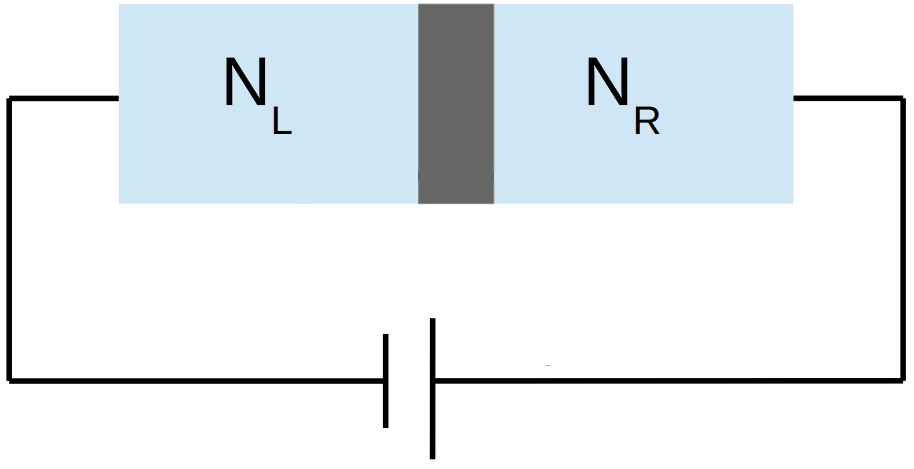
\includegraphics[width=0.5\textwidth]{immagini/NIN_junction.png}
\end{figure}
\hspace{-0.6cm}L'idea è che, a causa dell'effetto tunnel, esista una probabilità non nulla che un elettrone passi dal lead sinistro a quello destro o viceversa.\\
Come descriviamo quantisticamente questo processo? L'idea è partire dall'Hamiltoniana complessiva del sistema, che consiste nell'Hamiltoniana del lead sinistro, quella del lead destro e un termine di tunneling:
\begin{equation*}
    H=H_L + H_R + H_T
\end{equation*}
Poiché sia il lead sinistro che quello destro sono metalli normali, le rispettive Hamiltoniane sono semplicemente le Hamiltoniane in seconda quantizzazione che descrivono gli elettroni liberi in un metallo, con i consueti operatori di creazione e distruzione. Per distinguere i due lead utilizzeremo l'indice $\vb{k}$ per il lead sinistro e l'indice $\vb{q}$ per quello destro. Si ha quindi
\begin{equation*}
    H_L
    =
    \sum_{\vb{k}, \sigma}
    \varepsilon^{\vphantom{\dag}}_{\vb{k},\sigma}
    c^{\dag}_{\vb{k}, \sigma}
    c^{\vphantom{\dag}}_{\vb{k}, \sigma}
    \qq{,}
    H_R
    =
    \sum_{\vb{q}, \sigma}
    \varepsilon^{\vphantom{\dag}}_{\vb{q},\sigma}
    c^{\dag}_{\vb{q}, \sigma}
    c^{\vphantom{\dag}}_{\vb{q}, \sigma}
\end{equation*}
dove $\varepsilon_{\vb{k},\sigma}$ e $\varepsilon_{\vb{q},\sigma}$ sono i livelli energetici degli elettroni liberi nel metallo, esplicitamente dati da
\begin{equation*}
    \varepsilon_{\vb{k},\sigma}
    =\frac{\hbar^2 k^2}{2m}
    \qq{,}
    \varepsilon_{\vb{q},\sigma}
    =\frac{\hbar^2 q^2}{2m}
\end{equation*}
Dobbiamo poi descrivere, in seconda quantizzazione, la possibilità che gli elettroni attraversino la barriera per effetto tunnel:
\begin{equation*}
    H_T
    = \sum_{\vb{k}, \vb{q}, \sigma} T_{\vb{k}, \vb{q}} c^{\dag}_{\vb{k}, \sigma} c^{\vphantom{\dag}}_{\vb{q}, \sigma}
    + \text{h.c.}
\end{equation*}
Se partissimo da un'Hamiltoniana non scritta in seconda quantizzazione, ma in termini di energia cinetica e potenziale, dovremmo introdurre esplicitamente una barriera di potenziale caratterizzata da altezza e larghezza e successivamente derivarne autostati e autovalori. Qui invece stiamo già lavorando direttamente nella formulazione in seconda quantizzazione, in cui gli effetti della barriera, altezza, spessore, ecc., sono tutti incorporati nel coefficiente $T_{\vb{k},\vb{q}}$, che descrive essenzialmente la probabilità o l'ampiezza di transizione di un elettrone da un lato all'altro della giunzione.\\
Il processo di tunneling consiste nell'annichilazione di un elettrone da un lato della barriera e nella creazione di un elettrone dall'altro lato. L'Hamiltoniana che descrive questo processo\mn{Stiamo assumendo che gli elettroni fluiscano dal lead sinistro a quello destro; se la corrente fluisse nel verso opposto, gli operatori sarebbero invertiti.} è quindi un'Hamiltoniana che crea, ad esempio, un elettrone con momento $\vb{q}$ e spin $\sigma$ nel lead destro e annichila un elettrone con momento $\vb{k}$ e lo stesso spin nel lead sinistro, assumendo che il processo di tunneling non modifichi lo spin dell'elettrone.\\
Si tratta quindi di un operatore che distrugge un elettrone su un lato della giunzione e ne crea uno sull'altro lato, descrivendo così il processo di tunneling. Inoltre compare un coefficiente che descrive l'ampiezza di probabilità del processo oppure, se vogliamo, il costo energetico associato a esso. Questo coefficiente è indicato con $T$, da \textit{transmission}, e in generale dipende dai momenti della particella annichilata e di quella creata.\\
Dobbiamo poi sommare su tutti i possibili valori di $\vb{k}$ e $\vb{q}$ nei due elettrodi e, poiché assumiamo che lo spin venga conservato nel tunneling, non è necessario distinguere spin differenti nei due lati. Naturalmente bisogna anche aggiungere il termine hermitiano coniugato, che descrive il processo inverso.\\
Questa Hamiltoniana complessiva costituisce quindi un semplice modello che, in seconda quantizzazione, esprime la possibilità di tunneling elettronico tra i due elettrodi.\\
Se consideriamo un metallo normale a temperatura nulla, sappiamo che la densità degli stati è una funzione a gradino fino al livello di Fermi. Se supponiamo inoltre che i due elettrodi siano identici, essi avranno lo stesso livello di Fermi e la stessa densità degli stati. Possiamo quindi rappresentare la situazione nel modo seguente:
\begin{figure}[H]
    \centering
    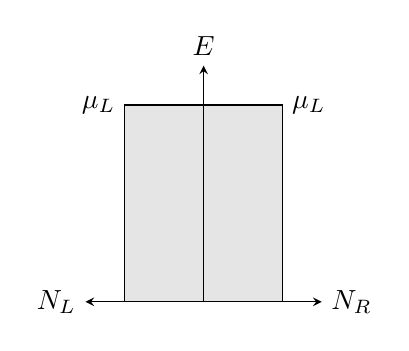
\begin{tikzpicture}
        %densità degli stati
        \draw[fill=gray!20!] (-1,0) rectangle (1,2.5);
        %assi
        \draw[-stealth] (0,0) -- (0,3) node[above] {$E$};
        \draw[stealth-stealth] (-1.5,0) node[left] {$N_L$}-- (1.5,0) node[right] {$N_R$};
        \node[left] at (-1,2.5) {$\mu_L$};
        \node[right] at (1,2.5) {$\mu_L$};
    \end{tikzpicture}
\end{figure}
\hspace{-0.6cm}L'Hamiltoniana descrive un processo in cui una particella viene distrutta da un lato e creata dall'altro, quindi un processo che trasferisce un elettrone da un elettrodo all'altro conservando l'energia.\\
Bisogna però verificare se, nell'altro elettrodo, siano disponibili livelli energetici liberi: se un livello è già occupato, l'elettrone non può occuparlo. Nella configurazione sopra illustrata il processo non è possibile, perché i due elettrodi sono identici, si trovano a temperatura nulla e tutti i livelli fino al livello di Fermi risultano occupati.\\
In questo caso, cioè in assenza di tensione applicata e a temperatura nulla, non può quindi avvenire tunneling: gli elettroni di un lead non possono passare nell'altro perché i corrispondenti livelli energetici sono già occupati, in accordo con il principio di esclusione di Pauli.\\
Che cosa accade invece se applichiamo una differenza di potenziale? Applicare una tensione significa, di fatto, traslare i livelli energetici dei due elettrodi:
\begin{figure}[H]
    \centering
    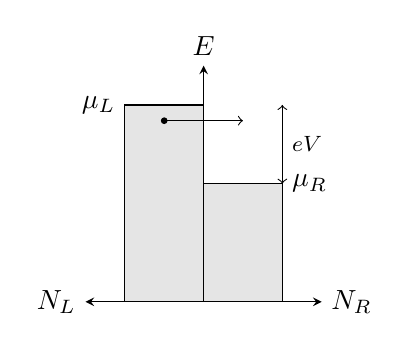
\begin{tikzpicture}
        %densità degli stati left lead
        \draw[fill=gray!20!] (-1,0) rectangle (0,2.5);
        %densità degli stati right lead
        \draw[fill=gray!20!] (0,0) rectangle (1,1.5);
        %assi
        \draw[-stealth] (0,0) -- (0,3) node[above] {$E$};
        \draw[stealth-stealth] (-1.5,0) node[left] {$N_L$}-- (1.5,0) node[right] {$N_R$};
        \node[left] at (-1,2.5) {$\mu_L$};
        \node[right] at (1,1.5) {$\mu_R$};

        %intensità del bias
        \draw[<->] (1,2.5) -- (1,1.5) node[midway,right] {\footnotesize$eV$};

        %elettrone che fa tunneling
        \filldraw (-0.5,2.3) circle (1pt);
        \draw[->] (-0.5,2.3) -- (0.5,2.3);
    \end{tikzpicture}
\end{figure}
\hspace{-0.6cm}Avremo quindi una densità degli stati traslata verso energie più alte da un lato e verso energie più basse dall'altro, in modo tale che i due potenziali chimici risultino separati da un'energia pari alla differenza di potenziale:
\begin{equation*}
    \mu_L - \mu_R = eV
\end{equation*}
In queste condizioni un elettrone nel lead sinistro può attraversare la barriera e occupare un livello energetico libero nel lead destro, proprio perché le due bande energetiche sono state traslate relativamente l'una rispetto all'altra.\\
Questo ci suggerisce immediatamente che, se calcoliamo la corrente che attraversa la giunzione, essa sarà nulla in assenza di tensione applicata, mentre diventerà diversa da zero quando esiste uno sbilancio tra le due bande energetiche, cioè quando viene applicata una differenza di potenziale.\\
Vediamo ora come scrivere esplicitamente tale corrente. Prima di tutto chiariamo la notazione utilizzata. Le energie $\varepsilon$ sono misurate rispetto al livello di Fermi di ciascun elettrodo, posto uguale a zero. Quindi $\varepsilon_L<0$ indica un livello occupato nell'elettrodo sinistro, mentre $\varepsilon_R>0$ indica un livello vuoto nell'elettrodo destro. La conservazione dell'energia richiede allora che
\begin{equation*}
    \varepsilon_R - \varepsilon_L
    =-eV
    =\mu_L - \mu_R
\end{equation*}
assumendo $e$ negativo.\\
L'idea è considerare l'Hamiltoniana di tunneling come una perturbazione rispetto alle Hamiltoniane dei due elettrodi, cioè assumere che i coefficienti $T_{\vb{k},\vb{q}}$, che quantificano l'interazione tra i due lead, siano molto più piccoli delle energie coinvolte:
\begin{equation*}
    |T_{\vb{k},\vb{q}}|
    \ll
    \varepsilon_{\vb{k},\sigma},
    \varepsilon_{\vb{q},\sigma}
\end{equation*}
Per determinare la probabilità per unità di tempo, cioè il rate, che un elettrone passi da un elettrodo all'altro a causa di questa perturbazione, utilizziamo la regola d'oro di Fermi. Dobbiamo quindi considerare tutte le possibili transizioni che conservano l'energia, la probabilità che lo stato iniziale sia occupato e quella che lo stato finale sia libero, sommando poi su tutti gli stati iniziali e finali possibili. Occorre inoltre includere un fattore 2 dovuto alla degenerazione di spin, poiché il processo non modifica lo spin.\\
L'espressione risultante è\mn{Con il simbolo $\sum_{R,L}$ intendiamo la somma su tutti i possibili valori di $\vb{q}$ e $\vb{k}$.}
\begin{equation*}
    \begin{split}
        W_{L \to R}
        &=
        2\frac{2\pi}{\hbar}
        \sum_{R,L}
        |T_{RL}|^2
        f_L(\varepsilon_L)
        \bigl[
            1-f_R(\varepsilon_R)
        \bigr]
        \delta(
            \varepsilon_L-eV-\varepsilon_R
        )
        \\
        W_{R \to L}
        &= 2\frac{2\pi}{\hbar} \sum_{R,L} |T_{RL}|^2 f_R(\varepsilon_R) \bigl[ 1 - f_L(\varepsilon_L) \bigr] \delta(\varepsilon_L - eV - \varepsilon_R)
    \end{split}
\end{equation*}
dove $f_L$ e $f_R$ sono le distribuzioni di Fermi dei due lead:
\begin{equation*}
    f_{\alpha}(\varepsilon_\alpha)
    =\frac{1}{1 + e^{\beta_\alpha \varepsilon_\alpha}}
    \qq{,}
    \alpha=L,R
\end{equation*}
Notiamo che stiamo esplicitamente indicando il lead perché, in generale, i due elettrodi possono trovarsi a temperature differenti. Se invece le temperature coincidono, possiamo semplicemente scrivere $f(\varepsilon)$ senza specificare il lead, perché in quel caso conta soltanto l'energia.\\
Una volta ottenute le probabilità di tunneling, possiamo ricavare facilmente la corrente totale, che è semplicemente la carica del portatore, $-e$, moltiplicata per la differenza tra i due rate:
\begin{equation*}
    I = -e ( W_{L \to R} - W_{R \to L} )
\end{equation*}
Sostituendo le espressioni esplicite dei due rate, otteniamo
\begin{equation*}
    I = -e \frac{4\pi}{\hbar} \sum_{R,L} |T_{RL}|^2 \bigl[ f_L(\varepsilon_L) - f_R(\varepsilon_R) \bigr] \delta( \varepsilon_L-eV-\varepsilon_R )
\end{equation*}
Passiamo ora al limite del continuo, sostituendo le somme con integrali sulle energie dei due lead e introducendo le corrispondenti densità degli stati $N_L(\varepsilon_L)$ e $N_R(\varepsilon_R)$:
\begin{equation*}
    I = -e \frac{4\pi}{\hbar} \int \dd{\varepsilon_R} N_R \int \dd{\varepsilon_L} N_L |T_{RL}|^2 \bigl[ f_L(\varepsilon_L) - f_R(\varepsilon_R) \bigr] \delta( \varepsilon_L-eV-\varepsilon_R )
\end{equation*}
Usando la delta di Dirac rimane un solo integrale, ad esempio su $\varepsilon_R$, mentre $\varepsilon_L$ viene sostituita con il valore imposto dalla conservazione dell'energia:
\begin{equation*}
    \varepsilon_L=eV+\varepsilon_R
\end{equation*}
Otteniamo quindi
\begin{equation*}
    I = -e \frac{4\pi}{\hbar} \int \dd{\varepsilon_R} N_R N_L |T_{RL}|^2
    \bigl[ f_L(eV+\varepsilon_R) - f_R(\varepsilon_R) \bigr]
\end{equation*}
Se assumiamo che la densità degli stati e l'ampiezza di tunneling siano praticamente costanti attorno al livello di Fermi, possiamo portarli fuori dall'integrale. Rimane così soltanto l'integrale della differenza delle due funzioni di Fermi:
\begin{equation*}
    \int \dd{\varepsilon_R} \bigl[ f_L(eV+\varepsilon_R) - f_R(\varepsilon_R) \bigr] = eV
\end{equation*}
È facile comprendere questo risultato graficamente a temperatura nulla:
\begin{figure}[H]
    \centering
    \begin{tikzpicture}
        %assi
        \draw[-stealth] (0,0) -- (0,2) node[left] {$f$};
        \draw[-stealth] (0,0) -- (5,0) node[right] {$\varepsilon$};
        \fill[pattern=north east lines] (2.3,0) rectangle (3.7,1.5);

        %fermi function left lead
        \draw[thick, blue]
        (0,1.5)
        --
        (3.7,1.5)
        node[midway, above] {\hspace{2cm}\footnotesize$f_R$}
        --
        (3.7,0)
        node[black, below] {\footnotesize$\varepsilon_R + eV$};

        \draw[thick, red]
        (0,1.5)
        --
        (2.3,1.5)
        node[midway, above] {\footnotesize$f_L$}
        --
        (2.3,0)
        node[black, below] {\footnotesize$\varepsilon_R$};
    \end{tikzpicture}
\end{figure}
\hspace{-0.6cm}Come si vede, la differenza tra le due funzioni di Fermi corrisponde semplicemente alla regione tratteggiata, che è un rettangolo di base $eV$ e altezza unitaria; l'integrale vale quindi semplicemente $eV$.\\
Tornando allora all'espressione della corrente, otteniamo\mn{È evidente che in tutto questo discorso non tornano i segni.}
\begin{equation*}
    I
    =\frac{4\pi e^2}{\hbar}N_LN_R|T_{RL}|^2V
    \equiv G_{NN}V
\end{equation*}
Si tratta semplicemente della legge di Ohm: la corrente è proporzionale alla differenza di potenziale applicata, con coefficiente di proporzionalità dato dalla conduttanza $G_{NN}$.\\
Questa è quindi una maniera di recuperare la legge di Ohm partendo da una descrizione microscopica quantistica degli elettroni nei due elettrodi. Ne segue che la caratteristica corrente--tensione della giunzione è lineare, con una pendenza determinata dalla conduttanza $G_{NN}$, che risulta proporzionale alla densità degli stati nei due lead e al quadrato dell'ampiezza di tunneling.
\subsection{Lead superconduttivi}
Vediamo ora che cosa accade quando i lead sono superconduttivi.\\
Consideriamo innanzitutto un processo di tunneling di singolo elettrone, cioè il passaggio di un singolo elettrone attraverso la giunzione. Perché un tale processo possa avvenire, è necessario rompere una coppia di Cooper, dalla quale otteniamo due elettroni. Come abbiamo già visto il costo energetico associato a ciò è pari a $2\Delta$, perché i livelli disponibili per ciascun elettrone si trovano a un'energia $\Delta$ sopra lo stato fondamentale.\\
Dobbiamo allora riesprimere tale stato elettronico in termini delle opportune eccitazioni del superconduttore. Esprimiamo allora l'operatore di creazione dell'elettrone $c^{\dag}_{\vb{k},\uparrow}$ in termini degli operatori di creazione e distruzione delle eccitazioni:
\begin{equation*}
    c^{\dag}_{\vb{k},\uparrow}
    =
    u^{\vphantom{\dag}}_{\vb{k}} b^{\dag}_{\vb{k},\uparrow}
    +
    \nu^{\vphantom{\dag}}_{\vb{k}} b^{\vphantom{\dag}}_{-\vb{k},\downarrow}
\end{equation*}
Se il superconduttore si trova nel suo stato fondamentale, il secondo termine fornisce un contributo nullo e il processo genera una corrente proporzionale a $|u_{\vb{k}}|^2 |T_{\vb{k},\vb{q}}|^2$.\\
Il significato fisico del fattore $|u_{\vb{k}}|^2$ è che esso rappresenta la probabilità che lo stato $\ket*{\vb{k}}$ non sia occupato nella funzione d'onda BCS e che quindi possa accogliere un elettrone incidente.\\
A prima vista sembrerebbe quindi che la corrente di tunneling dipenda sia dalla natura dello stato fondamentale superconduttivo sia dalla densità degli stati eccitati disponibili. Tuttavia ciò non è corretto.\\
Ricordiamo che le eccitazioni possiedono una dispersione parabolica. Se fissiamo un certo valore di $E_{\vb{k}}$, lo stesso valore dell'energia può essere ottenuto sia per $\xi_{\vb{k}}$ che per $-\xi_{\vb{k}}$. In altre parole, a causa della struttura dello spettro delle eccitazioni, possiamo avere due eccitazioni, che indichiamo con $E_{\vb{k}}$ ed $E_{\vb{k}'}$, coincidenti quando $\xi_{\vb{k}'}=-\xi_{\vb{k}}$.\\
Se allora adesso consideriamo l'operatore di creazione dell'elettrone $c^{\dag}_{\vb{k}',\uparrow}$, che crea un elettrone nello stato a singola particella $(\vb{k}',\uparrow)$, e analogamente a prima lo esprimiamo in termini degli operatori di creazione e distruzione delle eccitazioni, è facile vedere che il tunneling verso $\vb{k}'$ contribuisce con una corrente proporzionale a $|u_{\vb{k}'}|^2 |T_{\vb{k}',\vb{q}}|^2$.\\
Se però adesso utilizziamo l'\eqrefcustom{eq:coefficiente_u_BCS} e l'\eqrefcustom{eq:coefficiente_nu_BCS}, osserviamo che si ha
\begin{equation*}
    |u_{\vb{k}'}|^2
    =\frac{1}{2} \biggl( 1 + \frac{ \xi_{\vb{k}'} }{ \sqrt{ \xi_{\vb{k}'}^2+|\Delta|^2 } } \biggr)
    =\frac{1}{2} \biggl( 1 - \frac{ \xi_{\vb{k}} }{ \sqrt{ \xi_{\vb{k}}^2+|\Delta|^2 } } \biggr)
    \equiv |\nu_{\vb{k}}|^2
\end{equation*}
dove $|\nu_{\vb{k}}|^2$ rappresenta la probabilità che tale livello sia occupato nello stato fondamentale BCS.\\
Possiamo inoltre assumere ragionevolmente che $|T_{\vb{k},\vb{q}}|^2 = |T_{\vb{k}',\vb{q}}|^2$, dato che $k$ e $k'$ si trovano entrambi nelle vicinanze dello stesso punto della superficie di Fermi.\\
Questo significa che la probabilità che il livello corrispondente a $\vb{k}'$ sia libero per il tunneling coincide con la probabilità che lo stato con $\xi$ opposto sia occupato:
\begin{equation}
    |u_{\vb{k}'}|^2
    |T_{\vb{k}'\vb{q}}|^2
    =
    |\nu_{\vb{k}}|^2
    |T_{\vb{k}\vb{q}}|^2
    \label{eq:probability_tunneling_k'}
\end{equation}
Di conseguenza, se vogliamo valutare la probabilità totale che esista uno stato disponibile corrispondente a un certo valore di $\vb{k}$, dobbiamo sommare il contributo $|u_{\vb{k}}|^2 |T_{\vb{k},\vb{q}}|^2$, associato a $\xi_{\vb{k}}$, con il contributo $|u_{\vb{k}'}|^2 |T_{\vb{k}',\vb{q}}|^2$.\\
Esistono quindi due processi indipendenti, che derivano direttamente dalla particolare struttura dello spettro delle eccitazioni superconduttive. Complessivamente, la probabilità che un singolo elettrone venga trasferito nello stato a singola particella $(\vb{k},\uparrow)$, quando il superconduttore si trova nello stato fondamentale BCS, è data da
\begin{equation*}
    |u_{\vb{k}}|^2 |T_{\vb{k},\vb{q}}|^2 + |u_{\vb{k}'}|^2 |T_{\vb{k}',\vb{q}}|^2
\end{equation*}
Usando l'\eqrefcustom{eq:probability_tunneling_k'}, possiamo riscrivere questa espressione come
\begin{equation*}
    ( |u_{\vb{k}}|^2 + |\nu_{\vb{k}}|^2 ) |T_{\vb{k},\vb{q}}|^2
    =|T_{\vb{k},\vb{q}}|^2
\end{equation*}
dove abbiamo utilizzato la condizione di normalizzazione dello stato fondamentale BCS, $|u_{\vb{k}}|^2 + |\nu_{\vb{k}}|^2 = 1$.\\
Questa è una conseguenza notevole, perché ci dice che la corrente di tunneling risultante non dipende esplicitamente dai coefficienti che compaiono nello stato fondamentale BCS, ma soltanto dall'ampiezza di tunneling.
\subsection{Modello a semiconduttore per un superconduttore}
Quest'ultima osservazione è particolarmente importante, perché il passo successivo consiste nel valutare la corrente. Per farlo dobbiamo applicare la regola d'oro di Fermi e costruire un quadro analogo a quello introdotto nel caso dei metalli normali.\\
Questo tipo di descrizione viene spesso chiamato \emph{modello a semiconduttore} del superconduttore: quando si studiano le correnti nei dispositivi superconduttivi, si considera infatti la densità degli stati e i possibili processi di tunneling da un lato all'altro della giunzione, tenendo conto del gap energetico. Nel caso di un metallo normale questo procedimento è semplice, perché la densità degli stati ha una struttura molto semplice. Nel caso di un superconduttore, invece, la situazione è più complessa: nello stato fondamentale BCS gli elettroni formano coppie di Cooper e, quando tali coppie vengono rotte, compaiono le quasiparticelle, che possiedono una propria densità degli stati.\\
Quando consideriamo la corrente di tunneling dobbiamo necessariamente coinvolgere questi stati eccitati, perché il tunneling di singolo elettrone richiede la rottura di una coppia di Cooper e bisogna quindi capire in quali stati possano andare gli elettroni risultanti dalla rottura della coppia.\\
Il fatto che i processi di tunneling associati alla rottura di una coppia di Cooper non dipendano esplicitamente dai coefficienti che compaiono nello stato fondamentale BCS implica che, se vogliamo costruire una descrizione analoga a quella utilizzata per i semiconduttori, possiamo utilizzare un modello che coinvolga soltanto i livelli energetici eccitati, senza mantenere memoria esplicita dello stato fondamentale BCS.\\
Questo modello, utilizzato esclusivamente per descrivere i processi di tunneling elettronico, prende il nome di \emph{modello a semiconduttore per un superconduttore}. Vediamo qualitativamente come funziona:
\begin{figure}[H]
    \centering
    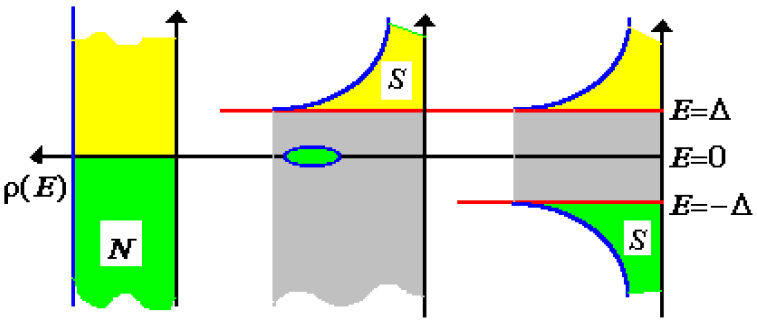
\includegraphics[width=0.8\textwidth]{immagini/semiconductor_model.png}
    \caption*{Rappresentazione a singola particella della densità degli stati di un superconduttore: quasiparticelle libere appartenenti a due bande. Una banda di coppie legate a energia $\Delta$ sotto il livello di Fermi e una banda di ``coppie rotte'' a energia $\Delta$ sopra il livello di Fermi. Rompere una coppia significa eccitare una quasiparticella sopra il gap. Il costo energetico per creare una ``lacuna'' nella banda inferiore e una quasiparticella nella banda superiore è pari a $2\Delta$.}
\end{figure}
\hspace{-0.6cm}A sinistra vediamo la struttura degli stati di un metallo normale: tutti i livelli fino al livello di Fermi (assunto come zero dell'energia) sono occupati, mentre quelli sopra il livello di Fermi sono vuoti.\\
Nel caso del superconduttore sappiamo invece che la densità degli stati possiede l'andamento caratteristico già discusso: compare un gap energetico e, vicino ai bordi del gap, la densità degli stati diverge prima di decrescere nuovamente.\\
L'immagine sulla destra rappresenta proprio il modello a semiconduttore del superconduttore. In essa compare la dipendenza delle energie eccitate dall'energia, ma — almeno a temperatura nulla — tali stati non sono occupati, perché tutte le particelle si trovano condensate nello stato fondamentale BCS.\\
Osserviamo inoltre che in questa rappresentazione lo stato fondamentale BCS non compare esplicitamente.\mn{Nel quadro a singola particella l'energia dello stato fondamentale BCS non compare nemmeno nel diagramma dei livelli energetici. Si tratta di un modello estremamente semplificato, utile esclusivamente per descrivere processi di tunneling a singolo elettrone, che risultano ``orizzontali'' quando i potenziali chimici dei due metalli vengono traslati per tenere conto della differenza di potenziale applicata.}
Un modo schematico per ricordare l'esistenza dello stato fondamentale è il ``blob'' rappresentato attorno all'energia zero nella figura centrale: esso indica semplicemente che tutti gli elettroni si trovano condensati altrove, cioè nello stato BCS. Le coppie di Cooper non partecipano direttamente al processo di tunneling di singolo elettrone.\\
Nel modello a semiconduttore ciò che si fa è passare dalla densità delle eccitazioni a una densità degli stati ottenuta riproducendo specularmente, anche per energie negative, la densità degli stati delle eccitazioni superconduttive. L'idea è quindi descrivere gli elettroni che formano lo stato fondamentale BCS come una sorta di mare di Fermi di stati occupati al di sotto del gap energetico.\\
Per capire perché questa costruzione abbia senso, immaginiamo di diminuire progressivamente il valore del gap $\Delta$ fino a portarlo a zero. Se partiamo da una densità degli stati superconduttiva e ne consideriamo la riproduzione speculare anche per energie negative, vediamo che, nel limite $\Delta \to 0$, il gap si chiude e la divergenza ai bordi scompare: la densità degli stati tende semplicemente a un valore costante uguale a quello di un metallo normale. In altre parole, se immaginassimo di osservare questo processo come un filmato, passando gradualmente da un valore finito di $\Delta$ fino a $\Delta=0$, vedremmo il diagramma trasformarsi gradualmente nella struttura tipica di un metallo normale.\\
Questo è il motivo per cui, nel modello a semiconduttore, si introduce una copia speculare della densità degli stati superconduttiva anche per energie negative: in questo modo il modello si riconduce naturalmente al caso normale quando il gap tende a zero.\\
Utilizzeremo questa rappresentazione per descrivere i processi di corrente di tunneling, in maniera analoga a quanto si fa nei semiconduttori. Anche nei semiconduttori, infatti, il trasporto è descritto in termini di quasiparticelle (elettroni e lacune) e la corrente deriva da processi di annichilazione di particelle da un lato e creazione dall'altro. Dal punto di vista concettuale, i processi che stiamo considerando qui sono dello stesso tipo.
\subsection{Giunzione Normale--Isolante--Superconduttore (NIS)}
Vediamo ora come utilizzare questo modello a semiconduttore per derivare la corrente tunnel. Il primo caso che consideriamo è una giunzione formata da un lead normale, uno strato isolante e un superconduttore. Se utilizziamo il modello a semiconduttore, il diagramma della densità degli stati assume la forma seguente:
\begin{figure}[H]
    \centering
    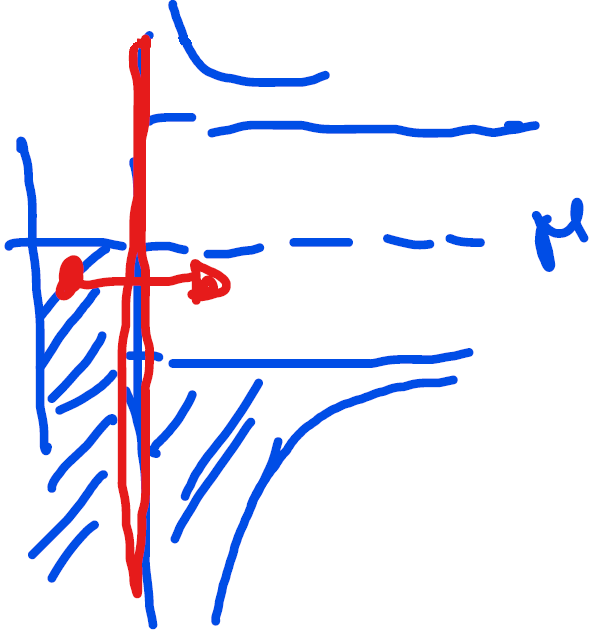
\includegraphics[width=0.3\textwidth]{immagini/NIS_junction_no_bias.png}
    \hspace{1cm}
    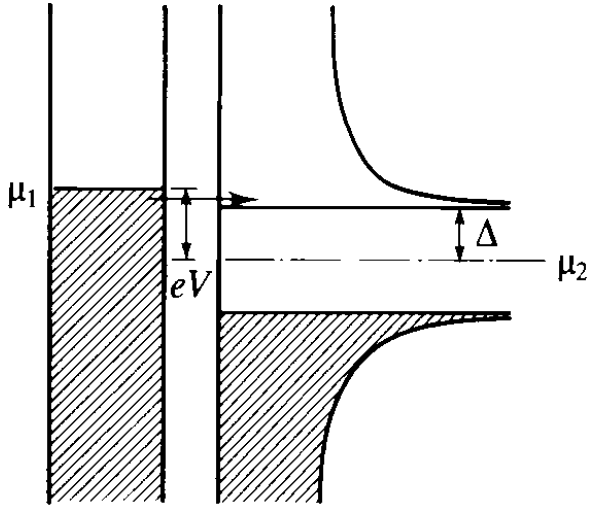
\includegraphics[width=0.4\textwidth]{immagini/NIS_junction.png}
    \caption*{(a) Tunneling N-S a $T=0$ in assenza di tensione applicata. (b) Tunneling N-S a $T=0$, con tensione di bias appena superiore alla soglia di conduzione, cioè con $eV$ leggermente maggiore del gap energetico $\Delta$. La freccia orizzontale rappresenta elettroni provenienti dal lato sinistro che tunnelano verso stati vuoti sul lato destro.}
\end{figure}
\hspace{-0.6cm}Sul lato sinistro abbiamo il metallo normale, mentre sul lato destro il superconduttore. Si noti che è stata applicata una tensione che trasla le due bande energetiche, perché altrimenti la situazione sarebbe quella mostrata nella figura (a). In queste condizioni non avremmo alcuna corrente, perché un elettrone presente nel metallo normale non potrebbe passare dall'altro lato: nel superconduttore non esistono infatti livelli disponibili a causa del gap energetico.\\
Possiamo avere una corrente soltanto applicando una differenza di potenziale, come nella figura (b), in modo da traslare le bande del superconduttore verso energie più basse e rendere possibili transizioni orizzontali dal metallo normale al superconduttore. In questo caso ciascun elettrone del metallo normale vede infatti un livello di quasiparticella disponibile nel superconduttore.\\
Devono quindi essere soddisfatte due condizioni:
\begin{itemize}[leftmargin=0.5cm]
    \item il livello energetico deve esistere;
    \item tale livello deve essere vuoto, in modo che l'elettrone possa occuparlo.
\end{itemize}
Questo implica immediatamente che nella caratteristica $I$--$V$ non osserveremo corrente per valori arbitrariamente piccoli della tensione applicata: è necessario che la tensione sia sufficientemente grande da permettere il tunneling di un elettrone. In altre parole, finché $eV<\Delta$ non avremo corrente; quando invece $eV$ supera $\Delta$, la corrente può iniziare a fluire.\\
Vediamo ora come si ottiene questo risultato. Utilizziamo ancora lo stesso modello per l'Hamiltoniana di tunneling e descriviamo la corrente tramite i rate di transizione $W_{L \to R}$ e $W_{R \to L}$ ottenuti con la regola d'oro di Fermi. La corrente totale sarà quindi
\begin{equation*}
    I_{NS}
    =
    I_{N \to S}
    -
    I_{S \to N}
\end{equation*}
Cominciamo valutando il primo termine, cioè la corrente che fluisce dal metallo normale al superconduttore. Sottolineiamo che qui non intervengono coppie di Cooper: compaiono soltanto quasiparticelle, che obbediscono alla statistica di Fermi e la cui occupazione è descritta dalla distribuzione di Fermi.\\
Procedendo esattamente come nel caso precedente, otteniamo\mn{Rispetto alle slide ho riportato una modifica. Infatti lì compare esplicitamente il fattore con la radice derivante dalla DOS del superconduttore, ma compare anche $N_R(E_R)$. Siccome $N_R$ dipende da $E_R$ solo se al suo interno c'è la radice, allora è più chiaro scrivere direttamente $N_R(E_R)$, che è la densità degli stati del superconduttore, invece di scrivere la radice e poi $N_R$.}
\begin{equation*}
    \begin{split}
        I_{N \to S}
        &=
        -e
        \frac{4\pi}{\hbar}
        \int
        \dd{\varepsilon_L}
        \int
        \dd{E_R}
        \Bigl\{
            |T_{LR}|^2
            N_L(\varepsilon_L)
            f_L(\varepsilon_L)
        \Bigr.
        \\
        & \hphantom{=
        -e
        \frac{4\pi}{\hbar}
        \int
        \dd{\varepsilon_L}
        \int
        \dd{E_R}}
        \Bigl.
        \times
        N_R(E_R)
        \bigl[
            1-f_R(E_R)
        \bigr]
        \delta(
            \varepsilon_L-eV-E_R
        )
        \Bigr\}
    \end{split}
\end{equation*}
Osserviamo che stiamo usando simboli differenti per i due lead: sul lato sinistro abbiamo un metallo normale e utilizziamo quindi la notazione $\varepsilon_L$, mentre sul lato destro abbiamo le eccitazioni del superconduttore, indicate con $E_R$.\\
Dobbiamo inoltre considerare la densità degli stati nei due lead. Per il metallo normale abbiamo semplicemente $N_L(\varepsilon_L)$, mentre per il superconduttore dobbiamo usare la densità degli stati delle quasiparticelle:
\begin{equation*}
    N_R(E_R)
    =
    N_R(0)
    \frac{
        E_R
    }{
        \sqrt{
            E_R^2-\Delta^2
        }
    }
\end{equation*}
Dobbiamo poi includere i consueti fattori che selezionano gli stati inizialmente occupati e quelli finali disponibili. Gli stati inizialmente occupati sono descritti dal prodotto $N_L(\varepsilon_L)
f_L(\varepsilon_L)$, mentre gli stati finali disponibili sono descritti da $N_R(E_R) \bigl[ 1-f_R(E_R) \bigr]$.\\
Questa è soltanto la corrente che fluisce dal metallo normale al superconduttore. Se consideriamo il processo inverso, cioè il contributo alla corrente dal superconduttore verso il metallo normale, dobbiamo semplicemente scambiare il ruolo degli stati occupati e vuoti:
\begin{equation*}
    \begin{split}
        I_{S \to N}
        &=
        -e
        \frac{4\pi}{\hbar}
        \int
        \dd{\varepsilon_L}
        \int
        \dd{E_R}
        \Bigl\{
            |T_{LR}|^2
            N_L(\varepsilon_L)
            \bigl[
                1-f_L(\varepsilon_L)
            \bigr]
        \Bigr.
        \\
        & \hphantom{=
        -e
        \frac{4\pi}{\hbar}
        \int
        \dd{\varepsilon_L}
        \int
        \dd{E_R}}
        \Bigl.
        \times
        N_R(E_R)
        f_R(E_R)
        \delta(
            \varepsilon_L-eV-E_R
        )
        \Bigr\}
    \end{split}
\end{equation*}
La corrente totale risulta quindi
\begin{equation*}
    \begin{split}
        I_{NS}
        &=
        -e
        \frac{4\pi}{\hbar}
        \int
        \dd{\varepsilon_L}
        \int
        \dd{E_R}
        \Bigl\{
            |T_{LR}|^2
            N_L(\varepsilon_L)
            N_R(E_R)
        \Bigr.
        \\
        & \hphantom{=
        -e
        \frac{4\pi}{\hbar}
        \int
        \dd{\varepsilon_L}
        \int
        \dd{E_R}}
        \Bigl.
        \times
        \bigl[
            f_L(\varepsilon_L)
            -
            f_R(E_R)
        \bigr]
        \delta(
            \varepsilon_L-eV-E_R
        )
        \Bigr\}
    \end{split}
\end{equation*}
Usando la delta di Dirac possiamo eliminare uno dei due integrali, ad esempio quello su $\varepsilon_L$, ottenendo un integrale soltanto su $E_R$.\\
Inoltre, scrivendo esplicitamente la densità degli stati del superconduttore, otteniamo
\begin{equation*}
    \begin{split}
        I_{NS}
        &=
        -e
        \frac{4\pi}{\hbar}
        |T_{LR}|^2
        N_L(0)
        N_R(0)
        \\
        & \hphantom{=}
        \times
        \int_{-\infty}^{+\infty}
        \dd{E_R}
        \frac{
            E_R
        }{
            \sqrt{
                E_R^2-\Delta^2
            }
        }
        \bigl[
            f_L(eV+E_R)
            -
            f_R(E_R)
        \bigr]
    \end{split}
\end{equation*}
dove abbiamo assunto che l'ampiezza di tunneling e la densità degli stati siano praticamente costanti attorno al livello di Fermi.\\
A temperatura nulla, le funzioni di Fermi selezionano gli stati energetici compresi in una finestra di ampiezza $eV$. Tuttavia, nel superconduttore gli stati disponibili non iniziano da energia zero, ma da $\Delta$, perché la densità degli stati si annulla al di sotto del gap.\mn{Infatti, in principio le due funzioni di Fermi selezionano energie comprese tra zero e $-eV$, ma poiché la densità degli stati del superconduttore è nulla per energie minori di $\Delta$, rimane soltanto l'integrale compreso tra $\Delta$ e $-eV$.} Otteniamo quindi
\begin{equation*}
    \begin{split}
        I_{NS}
        &\approx
        -e
        \frac{4\pi}{\hbar}
        |T_{LR}|^2
        N_L(0)
        N_R(0)
        \int_{\Delta}^{-eV}
        \dd{E_R}
        \frac{
            E_R
        }{
            \sqrt{
                E_R^2-\Delta^2
            }
        }
        \\
        &=
        \frac{
            G_{NN}
        }{
            |e|
        }
        \sqrt{
            (eV)^2-\Delta^2
        }.
    \end{split}
\end{equation*}
Vediamo quindi che il risultato dell'integrale possiede un andamento a radice quadrata dipendente sia dal gap $\Delta$ sia dalla tensione applicata. A temperatura nulla, tale comportamento inizia soltanto quando $eV=\Delta$, come mostrato nella figura seguente:
\begin{figure}[H]
    \centering
    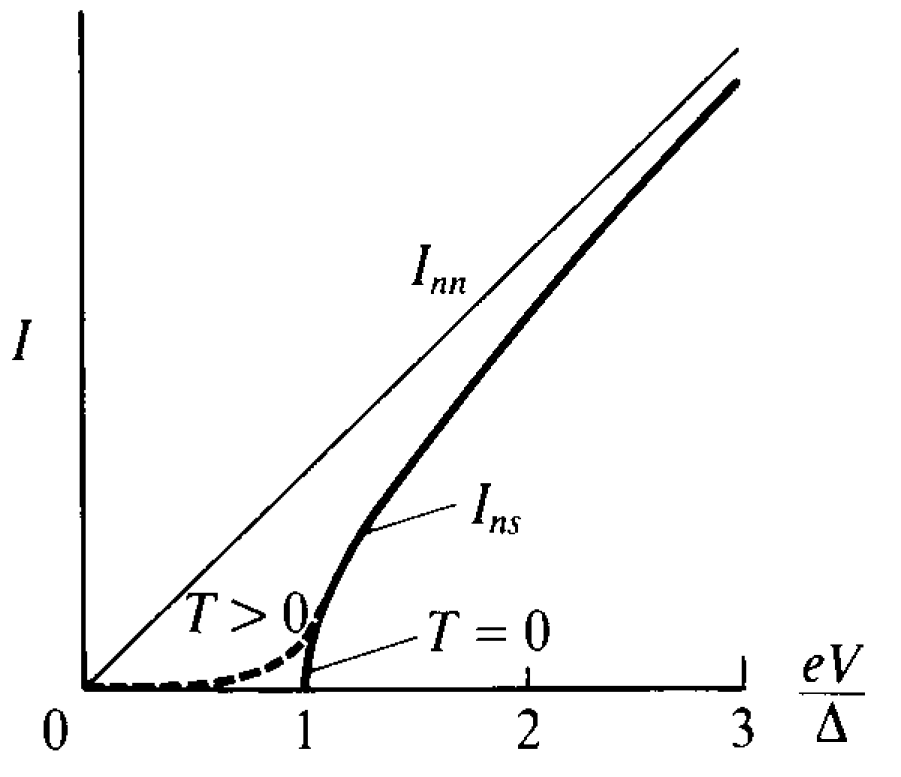
\includegraphics[width=0.45\textwidth]{immagini/IV_NIS.png}
\end{figure}
\hspace{-0.6cm}Come si vede, per $eV \gg \Delta$ si recupera nuovamente un comportamento lineare\mn{In tale regime il termine $\Delta$ all'interno della radice diventa trascurabile e si ottiene $\sqrt{(eV)^2}=eV$.}.\\
L'aspetto notevole è che il coefficiente davanti all'integrale è esattamente lo stesso che compare nella corrente quando entrambi i lead si trovano nello stato normale. Questo significa che, se la tensione applicata è molto maggiore del gap energetico, il sistema si comporta sostanzialmente come un metallo normale: la caratteristica $I$--$V$ torna lineare e con la stessa pendenza.\\
Riducendo invece la tensione applicata, la corrente risulta più piccola rispetto al caso normale e dipende in maniera non lineare da $eV$. Inoltre, per tensioni tali che $eV/\Delta<1$, la corrente si annulla completamente.\\
A temperatura finita la situazione cambia leggermente, perché in questo caso possono comparire stati occupati sopra il gap e stati vuoti al di sotto di esso, come illustrato nella figura seguente:
\begin{figure}[H]
    \centering
    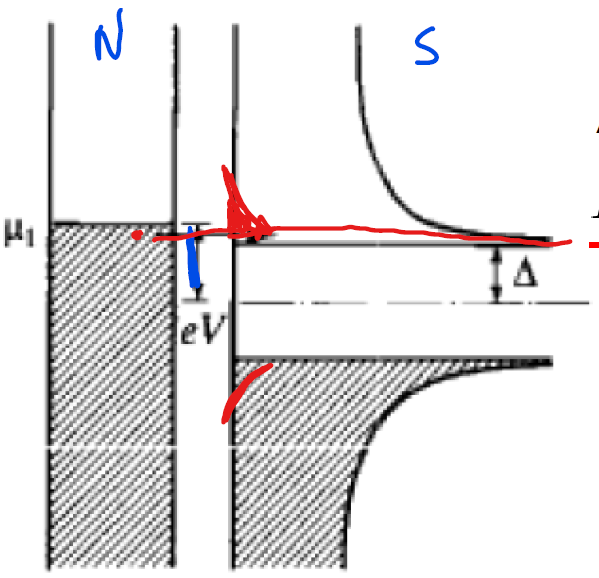
\includegraphics[width=0.4\textwidth]{immagini/finite_temperature_NIS.png}
\end{figure}
\hspace{-0.6cm}Analogamente a quanto avviene nei semiconduttori, a temperatura finita esistono livelli eccitati termicamente occupati. Ciò significa che possono verificarsi processi di tunneling anche per tensioni minori di $\Delta$.\\
Questo spiega perché nella caratteristica $I$--$V$ compare una piccola corrente anche per $eV<\Delta$, rappresentata nella figura dalla linea tratteggiata.\\
Possiamo anche valutare la conduttanza differenziale, che non è altro che la derivata della corrente rispetto alla tensione. Per $T=0$ si ottiene
\begin{equation*}
    \begin{split}
        \dv{I_{NS}}{V}
        &=
        e
        \frac{4\pi}{\hbar}
        N_L(0)
        |T_{LR}|^2
        \frac{N_R(0)|e|V}{\sqrt{(eV)^2-\Delta^2}}
    \end{split}
\end{equation*}
Osserviamo che questa funzione possiede essenzialmente la stessa forma funzionale della densità degli stati del superconduttore, con l'unica differenza che al numeratore compare $eV$ invece di $E$.\\
Questo significa che, se rappresentiamo la conduttanza differenziale in funzione di $eV/\Delta$, otteniamo un andamento identico a quello della densità degli stati del superconduttore, naturalmente valido soltanto per $eV>\Delta$:
\begin{figure}[H]
    \centering
    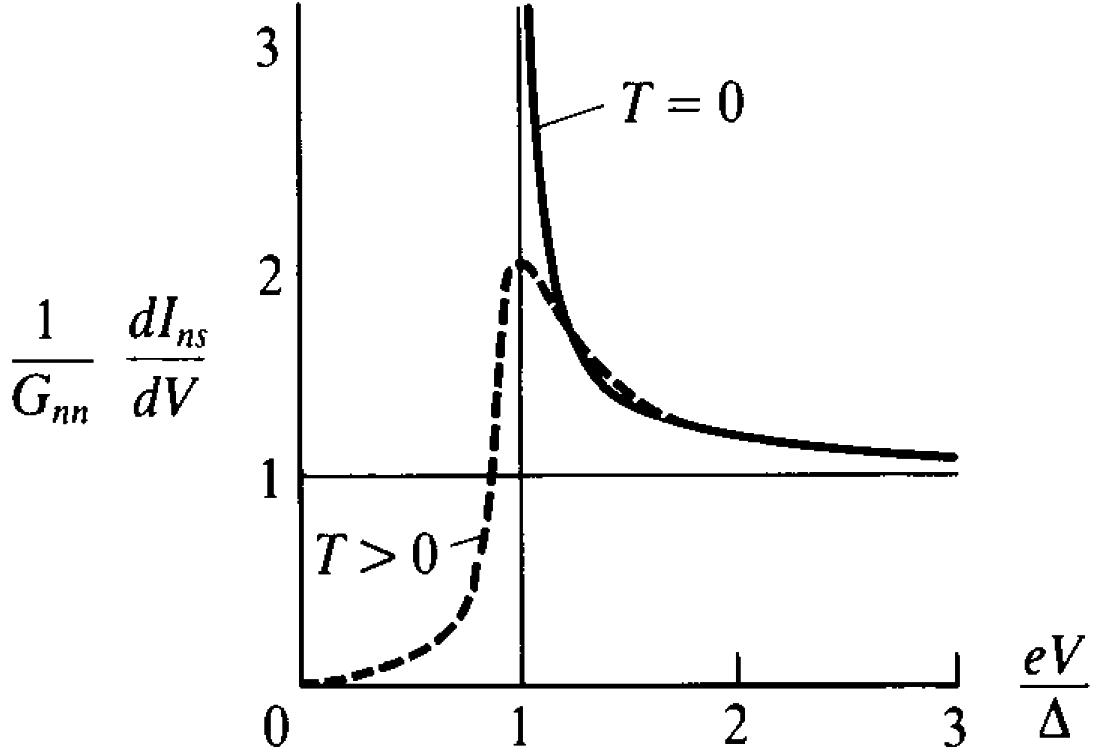
\includegraphics[width=0.5\textwidth]{immagini/differential_conductance_NIS.png}
\end{figure}
\hspace{-0.6cm}Idealmente, se fosse possibile lavorare esattamente a temperatura nulla, dalla misura della conduttanza differenziale potremmo ricavare direttamente la densità degli stati del superconduttore.\\
Naturalmente, negli esperimenti reali ci troviamo sempre a temperatura finita. Gli effetti termici modificano leggermente la regione con $eV/\Delta>1$ ed eliminano la divergenza che comparirebbe a temperatura nulla. In pratica, il comportamento della conduttanza differenziale rimane molto simile a quello ideale, ma il picco divergente viene sostituito da un massimo finito e smussato, che decresce rapidamente per tensioni più piccole.\\
Questo significa che, effettuando un esperimento di tunneling a temperature sufficientemente inferiori al gap, si osserva una conduttanza differenziale che riproduce molto bene la densità degli stati di un superconduttore, eccetto per la divergenza ideale.\\
\mn{Questa parte l'ho presa da \cite{Tinkham} e la aggiungo solo per completezza. La prof a lezione mostra solo l'espressione.}
Vediamo matematicamente da dove nasce questo comportamento non monotono. Consideriamo la conduttanza differenziale $\dv*{I}{V}$ in funzione della tensione:
\begin{equation*}
    G_{ns}
    =
    \dv{I_{ns}}{V}
    =
    G_{nn}
    \int_{-\infty}^{\infty}
    \dd{E}
    \frac{
        N_R(E)
    }{
        N_L(0)
    }
    \qty(
        -
        \pdv{
            f(E+eV)
        }{
            eV
        }
    ).
\end{equation*}
Poiché $-\pdv*{f(E+eV)}{eV}$ è una funzione a campana centrata attorno a $E=-eV$, con larghezza dell'ordine di $\sim 4kT$ e area unitaria, a temperatura finita la conduttanza misura in pratica una densità degli stati ``spalmata'' su un intervallo energetico dell'ordine di $\pm 2kT$, proprio a causa della larghezza della funzione peso.
\subsection{Giunzione Superconduttore--Isolante--Superconduttore (SIS)}
Consideriamo ora ill caso in cui entrambi i lead siano superconduttivi.\\
L'idea si comprende facilmente osservando la seguente struttura a bande. Ancora una volta, il punto fondamentale è che possiamo avere una corrente di tunneling soltanto se esistono stati occupati da un lato e stati vuoti dall'altro.
\begin{figure}[H]
    \centering
    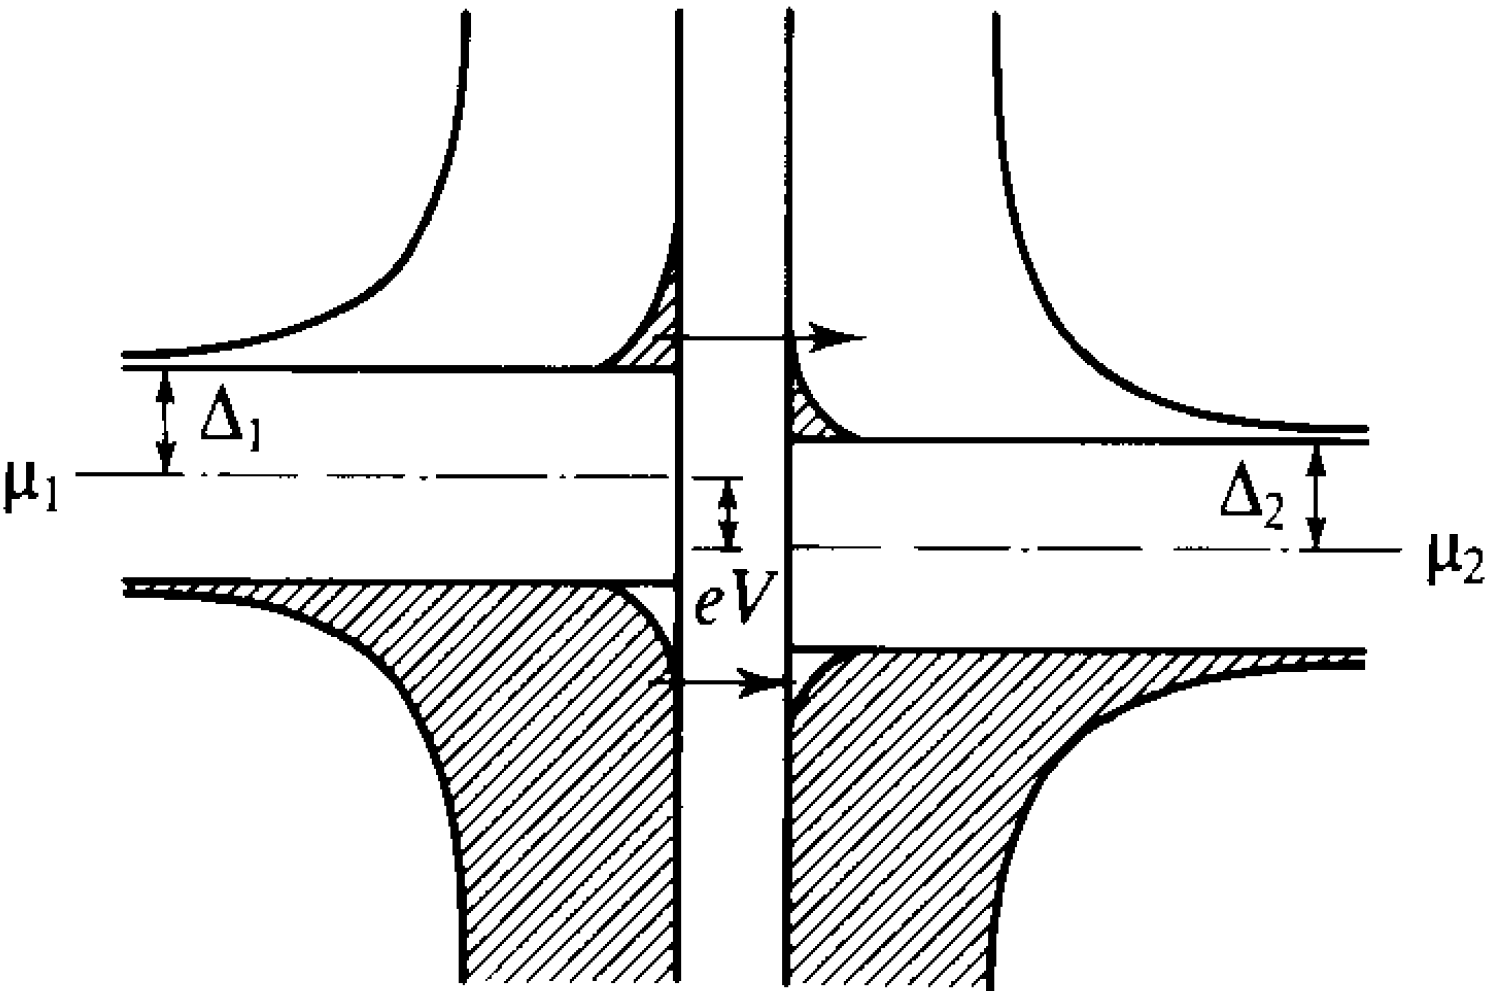
\includegraphics[width=0.55\textwidth]{immagini/SIS_junction.png}
\end{figure}
\hspace{-0.6cm}Questa figura rappresenta il caso di temperatura piccola ma finita: vicino alla sommità di quella che sarebbe la banda di valenza compaiono infatti alcuni livelli non occupati, mentre nel fondo della banda superiore si osservano alcune quasiparticelle termicamente eccitate.\\
In questa situazione possono verificarsi i processi illustrati nella figura. Possiamo avere elettroni che tunnelano da un lato all'altro anche per energie inferiori al gap, quando un elettrone presente da un lato passa in uno dei livelli disponibili dall'altro lato al di sotto del gap. Possiamo inoltre avere processi che coinvolgono stati eccitati su entrambi i lati della giunzione.\\
L'espressione della corrente è analoga a quella ottenuta nel caso precedente. Attraverso passaggi del tutto simili, e tenendo conto che ora entrambi i lead sono superconduttivi, si ottiene
\begin{equation*}
    \begin{split}
        I_{SS}
        &=
        -e
        \frac{4\pi}{\hbar}
        \int
        \dd{E_L}
        N_L
        \frac{
            |E_L|
        }{
            \sqrt{
                E_L^2-\Delta_1^2
            }
        }
        \int
        \dd{E_R}
        N_R
        \frac{
            |E_R|
        }{
            \sqrt{
                E_R^2-\Delta_2^2
            }
        }
        \\
        & \hphantom{=} \, 
        \times
        |T_{LR}|^2
        \bigl[
            f_L(E_L)
            -
            f_R(E_R)
        \bigr]
        \delta(
            E_L-eV-E_R
        )
        \\
        &=
        -e
        \frac{4\pi}{\hbar}
        |T_{LR}|^2
        N_L(0)
        N_R(0)
        \\
        & \hphantom{=} \,
        \times
        \int_{-\infty}^{+\infty}
        \dd{E}
        \frac{
            E
        }{
            \sqrt{
                E^2-\Delta_1^2
            }
        }
        \frac{
            E+eV
        }{
            \sqrt{
                (E+eV)^2-\Delta_2^2
            }
        }
        \bigl[
            f_L(E+eV)
            -
            f_R(E)
        \bigr]
    \end{split}
\end{equation*}
La caratteristica $I$--$V$ risultante ha il seguente aspetto:
\begin{figure}[H]
    \centering
    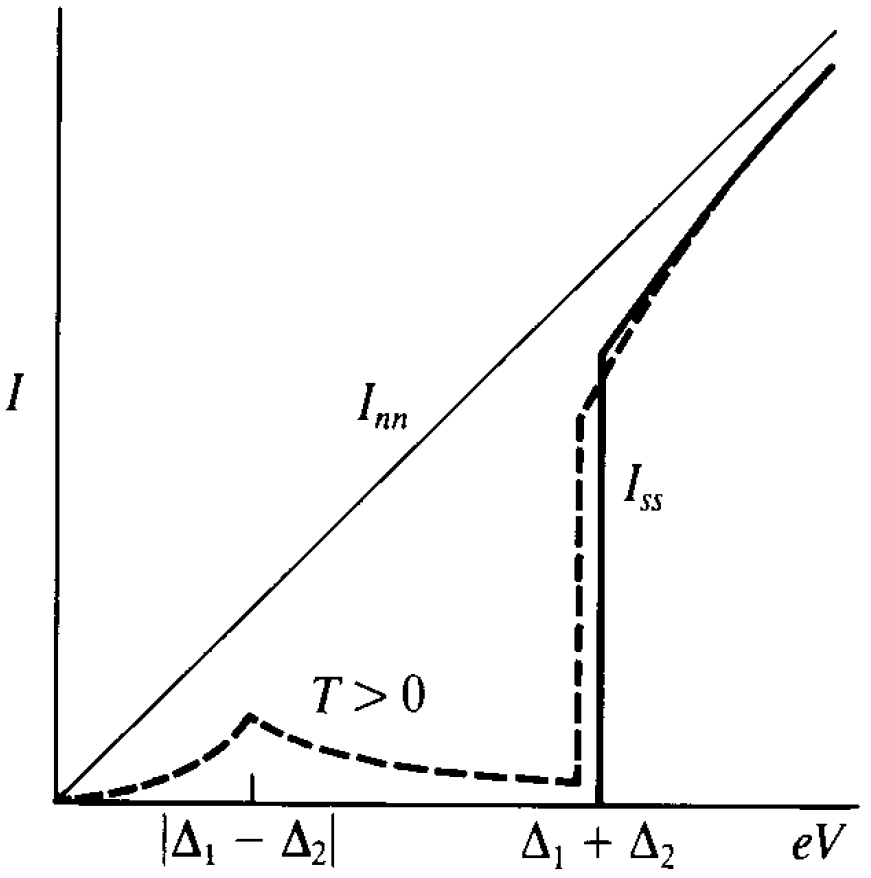
\includegraphics[width=0.45\textwidth]{immagini/IV_SIS.png}
\end{figure}
\hspace{-0.6cm}A temperatura nulla non compare alcuna corrente finché la tensione applicata non raggiunge la somma dei due gap energetici. Questo si comprende osservando il diagramma a bande nel caso $T=0$:
\begin{figure}[H]
    \centering
    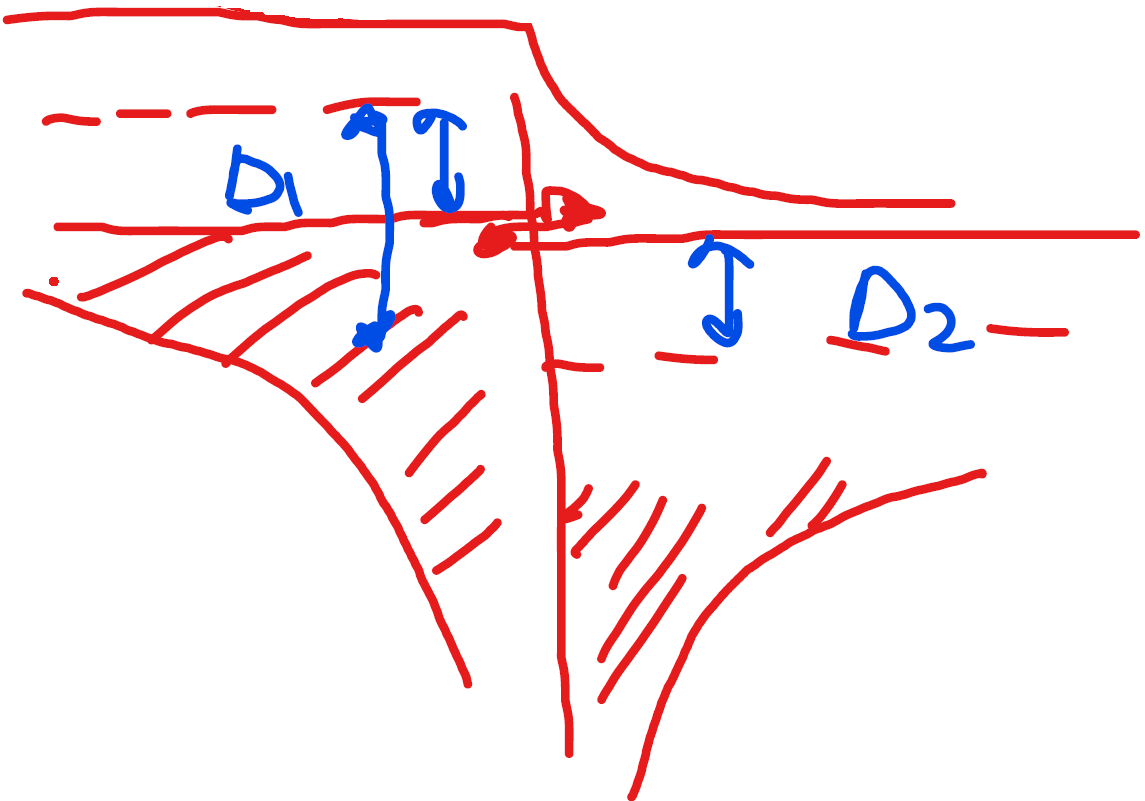
\includegraphics[width=0.4\textwidth]{immagini/SIS_junction_zero_temperature.png}
\end{figure}
\hspace{-0.6cm}Per avere una corrente di tunneling consiste un livello occupato deve poter tunnelare verso un livello disponibile dall'altro lato. Perché ciò avvenga, è necessario che la differenza di potenziale applicata sia tale da allineare opportunamente le bande energetiche, cioè $eV=\Delta_1+\Delta_2$.\\
A temperatura nulla, quindi, la corrente compare soltanto quando la tensione raggiunge la somma dei due gap. In questo caso si osserva un brusco aumento della corrente, perché appena questa condizione viene soddisfatta, gli elettroni di uno dei due superconduttori trovano immediatamente un grande numero di stati di quasiparticella disponibili nell'altro superconduttore.\\
Se invece la temperatura è finita, la corrente di tunneling assume l'andamento rappresentato dalla linea tratteggiata nella figura precedente: compare un comportamento non monotono con un massimo localizzato a un'energia pari alla differenza tra i due gap. Questo comportamento deriva dai differenti processi di tunneling che coinvolgono gli stati occupati termicamente.\\
Se siamo in grado di misurare sperimentalmente la caratteristica corrente--tensione e osserviamo una forma di questo tipo, possiamo ricavare direttamente i due gap $\Delta_1$ e $\Delta_2$. Infatti, il primo massimo della corrente si trova in corrispondenza di $|eV_1|=|\Delta_1-\Delta_2|$, mentre il brusco aumento della corrente si verifica invece per $|eV_2|=|\Delta_1+\Delta_2|$. Dai valori di tensione in cui compaiono questi due fenomeni possiamo quindi determinare i gap dei due superconduttori che formano la giunzione.\\
Vediamo ora qualitativamente perché compare questo comportamento:
\begin{figure}[H]
    \centering
    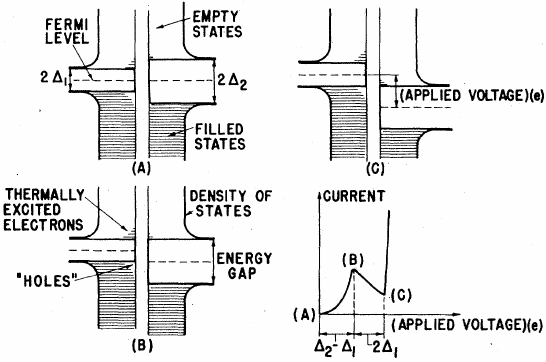
\includegraphics[width=0.9\textwidth]{immagini/SIS_junction_finite_temperature.png}
    %\caption*{Tunneling tra due superconduttori con gap energetici differenti a temperatura maggiore di $0^\circ$ K.     (a) Nessuna tensione applicata tra i due conduttori. (b) Applicando una tensione diventa energeticamente possibile per un numero sempre maggiore di elettroni eccitati termicamente fluire dal superconduttore con gap minore verso quello con gap maggiore. Alla tensione mostrata, tutti gli elettroni eccitati trovano stati disponibili sul lato destro. (c) Aumentando ulteriormente la tensione, non entrano in gioco nuovi elettroni e, poiché diminuisce il numero di stati accessibili per il tunneling, la corrente diminuisce al crescere della tensione. Quando la tensione diventa sufficientemente grande, gli elettroni al di sotto del gap nel superconduttore di sinistra trovano stati vuoti sul lato destro e si osserva un rapido aumento della corrente. (d) Andamento schematico della caratteristica corrente--tensione.}
\end{figure}
\hspace{-0.6cm}Il punto di partenza è la situazione rappresentata in (a). Abbiamo due superconduttori con gap differenti, $\Delta_1$ a sinistra e $\Delta_2$ a destra. I potenziali chimici sono allineati perché non è applicata alcuna tensione.\\
In questa configurazione esistono alcune eccitazioni termiche soltanto nel superconduttore con gap minore, perché nell'altro superconduttore l'energia richiesta per creare eccitazioni è più grande e quindi gli effetti termici risultano molto più piccoli.\\
In tali condizioni possiamo avere soltanto una piccola corrente dovuta a pochi livelli occupati che riescono a tunnelare verso stati disponibili sull'altro lato. Si tratta quindi di un effetto molto debole.\\
Successivamente aumentiamo la tensione applicata, passando alla situazione (b). I due potenziali chimici non risultano più allineati e gli elettroni eccitati termicamente trovano ora livelli energetici disponibili nell'altro superconduttore.\\
Osservando la figura (d), vediamo che la corrente cresce fino a raggiungere un massimo quando $eV = \Delta_1-\Delta_2$.  Questa configurazione corrisponde precisamente al caso illustrato in (b).\mn{Nota di ChatGPT: questo accade perché a questa tensione tutti i livelli occupati sul lato sinistro riescono a trovare stati disponibili sul lato destro, realizzando una sorta di condizione di risonanza. È per questo motivo che compare il massimo della corrente.}\\
Se aumentiamo ulteriormente la tensione, si raggiunge la situazione illustrata in (c). In questo caso i processi di tunneling precedenti non possono più verificarsi efficacemente, perché molti degli stati finali accessibili cadono all'interno del gap energetico dell'altro superconduttore.\\
Di conseguenza esiste una regione di tensioni superiori a $\Delta_1-\Delta_2$ in cui la corrente, invece di aumentare, diminuisce. Le due bande risultano infatti soltanto parzialmente sovrapposte e il numero di stati occupati che riescono a trovare livelli disponibili sull'altro lato si riduce. Questo è l'origine del comportamento non monotono della corrente.\\
Infine, aumentando ancora la tensione, si raggiunge la condizione $eV=\Delta_1+\Delta_2$. In questo caso tutti gli stati eccitati del superconduttore di sinistra trovano stati eccitati disponibili nel superconduttore di destra e si osserva quindi un brusco aumento della corrente.
\subsection{Scattering di Andreev}
Discutiamo ora un altro effetto identificato da Andreev, noto come scattering di Andreev. Nel seguito ne daremo una descrizione qualitativa.\\
Supponiamo di avere un'interfaccia metallo normale--superconduttore, senza alcuna barriera isolante.
\begin{figure}[H]
    \centering
    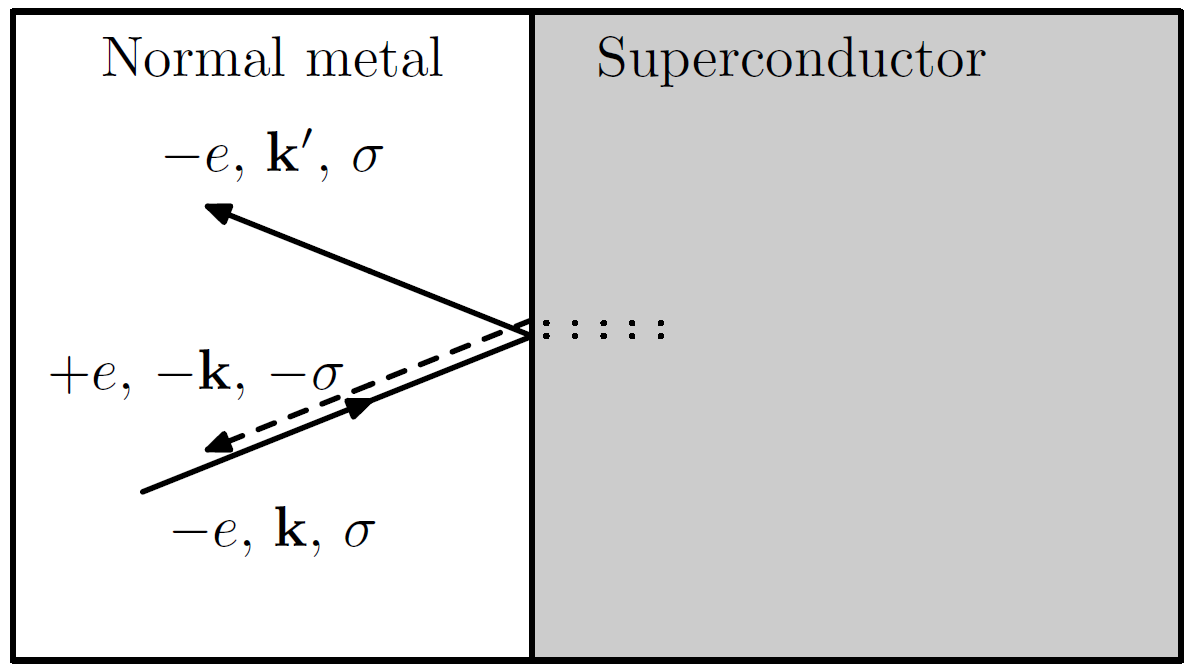
\includegraphics[width=0.4\textwidth]{immagini/Andreev_scattering.png}
\end{figure}
\hspace{-0.6cm}Sul lato sinistro abbiamo elettroni normali, mentre sul lato destro abbiamo coppie di Cooper.\\
Può accadere che un elettrone con carica $-e$, quantità di moto $\vb{k}$ e spin $\sigma$ si propaghi nel metallo normale e raggiunga la superficie del superconduttore. Se il superconduttore si trova nello stato fondamentale BCS, questo elettrone non può partecipare direttamente alla superconduttività, poiché non esistono stati disponibili a singola particella all'interno del gap energetico. In questo caso l'elettrone viene riflesso specularmente: la sua carica rimane invariata, così come il suo spin, mentre la quantità di moto cambia in modo tale da conservare la quantità di moto totale.\\
Esiste tuttavia un altro possibile processo, identificato da Andreev, che consiste nella combinazione dell'elettrone incidente con un secondo elettrone del metallo normale per formare una coppia di Cooper che entra nel superconduttore.\\
In questo caso, nel superconduttore compare una coppia di Cooper aggiuntiva, quindi una carica complessiva pari a $-2e$. Poiché la carica totale deve conservarsi, sul lato normale compare una lacuna (\textit{hole}), cioè una carica negativa mancante, che possiamo interpretare come una buca nel metallo normale.\\
Inoltre, per conservare la quantità di moto, dato che l'elettrone che entra nel superconduttore mantiene la propria quantità di moto, la lacuna riflessa deve avere quantità di moto $-\vb{k}$. Analogamente, per la conservazione dello spin, se l'elettrone entrato nel superconduttore possiede spin $\sigma$, la lacuna risultante deve avere spin opposto $-\sigma$.\\
Dal punto di vista qualitativo possiamo quindi descrivere questo processo come un elettrone incidente che colpisce l'interfaccia e una lacuna riflessa con carica opposta, quantità di moto opposta e spin opposto, che quindi si propaga all'indietro rispetto all'elettrone incidente.\\
Il risultato netto del processo è che due elettroni vengono trasferiti nel superconduttore, mentre sul lato normale avviene un processo equivalente all'annichilazione di un elettrone e alla creazione di una lacuna, il tutto nel rispetto della conservazione della carica.\\
Come si può osservare sperimentalmente questo effetto? Il punto fondamentale è il seguente. Consideriamo il processo di Andreev illustrato in figura:
\begin{figure}[H]
    \centering
    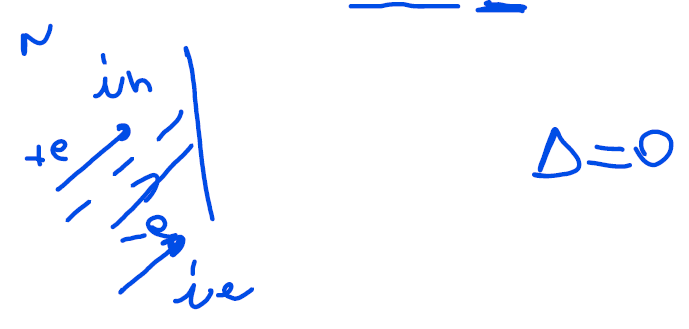
\includegraphics[width=0.4\textwidth]{immagini/Andreev_process.png}
\end{figure}
\hspace{-0.6cm}Nel metallo normale le lacune trasportano carica opposta e si propagano in direzione opposta rispetto all'elettrone incidente. Se quindi abbiamo un elettrone entrante che si muove in una certa direzione, esso produce una corrente in quella direzione; contemporaneamente, una lacuna che si muove nella direzione opposta genera anch'essa una corrente nello stesso verso dell'elettrone incidente.\\
Di conseguenza, questo processo produce una corrente pari al doppio della corrente che si avrebbe nel caso di un metallo normale oppure nel caso di un processo di tunneling ordinario indotto da una tensione sufficientemente grande da superare il gap energetico.\\
L'osservazione sperimentale di una corrente doppia rispetto a quella attesa nel caso $\Delta=0$ costituisce quindi una chiara evidenza dell'esistenza dei processi di Andreev.
\section{Effetto Josephson}
Finora abbiamo visto che cosa accade quando tra un metallo normale e un superconduttore, oppure tra due superconduttori, è presente uno strato isolante. Considerando la densità degli stati dei superconduttori, abbiamo essenzialmente analizzato quali processi possono avere luogo quando il tunneling attraverso la barriera isolante comporta la rottura delle coppie di Cooper.\\
Questo dà origine a particolari relazioni corrente--tensione, caratterizzate tipicamente dalla presenza di intervalli di tensione nei quali non scorre corrente. Il motivo è che il sistema deve fornire energia sufficiente per rompere almeno una o più coppie di Cooper affinché possa comparire una corrente. In questo caso, le singole quasiparticelle tunnelano indipendentemente attraverso la giunzione, poiché provengono dal condensato formato dalle coppie di Cooper.\\
Esiste tuttavia un altro fenomeno possibile, scoperto da Josephson nel 1962, noto come effetto Josephson. Esso consiste nel fatto che, invece di avere singoli elettroni che attraversano la giunzione, sono le coppie di Cooper a ``tunnelare'' attraverso la barriera.\mn{In realtà questa non è la descrizione più corretta del fenomeno. Più precisamente, ciò che avviene è la formazione di un unico condensato coerente modificato che coinvolge entrambi i superconduttori separati dalla barriera isolante.}\\
In questo processo compare una supercorrente, perché non avviene la rottura delle coppie di Cooper, nonostante non sia presente alcuna differenza di potenziale tra i due elettrodi.\\
Dal punto di vista qualitativo, ciò che accade è che la funzione d'onda elettronica penetra attraverso la barriera isolante, dando luogo a un accoppiamento coerente tra i due superconduttori. La descrizione teorica del fenomeno richiede quindi la formazione di uno stato coerente collettivo dell'intero sistema elettronico.\\
Nel seguito vedremo come descrivere quantitativamente questo effetto.
\subsection{Giunzione Josephson}
Consideriamo la giunzione Josephson più semplice che possiamo realizzare. Vedremo che questa non è l'unica possibilità, ma rappresenta la configurazione standard:
\begin{figure}[H]
    \centering
    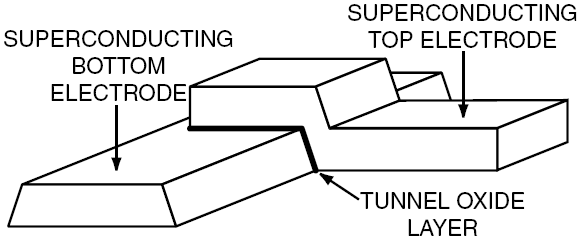
\includegraphics[width=0.5\textwidth]{immagini/Josephson_junction.png}
\end{figure}
\hspace{-0.6cm}Abbiamo due elettrodi superconduttivi, generalmente realizzati uno sopra l'altro. Tra i due strati superconduttivi è presente un ossido che svolge il ruolo di barriera isolante.\\
Tipicamente la giunzione viene realizzata con alluminio e l'ossido è $\rm Al_x O_y$, con $x \leq 2$ e $y \leq 3$. Lo spessore della barriera è soltanto di circa $2$--$3\;\rm nm$, mentre le dimensioni laterali tipiche sono dell'ordine di $0.1\times0.1\;\rm \mu m^2$ per le giunzioni più piccole e $1\times1\;\rm \mu m^2$ per quelle più grandi.\\
Naturalmente, le temperature alle quali questi sistemi operano devono essere tali da mantenere i materiali nello stato superconduttivo; tipicamente si lavora a $T \sim 20$--$30\;\rm mK$, mentre il gap energetico di questi materiali è dell'ordine di $200\;\mu\rm eV$. Il gap è quindi molto maggiore dell'energia termica associata alla temperatura operativa, che vale circa $3\;\mu\rm eV$.\\
Dal punto di vista schematico possiamo rappresentare la giunzione nel modo seguente:
\begin{figure}[H]
    \centering
    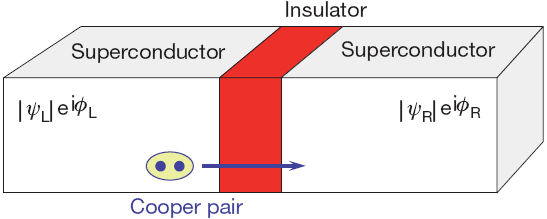
\includegraphics[width=0.5\textwidth]{immagini/Josephson_effect.png}
\end{figure}
\hspace{-0.6cm}Abbiamo dunque due superconduttori separati da uno strato isolante.\\
Supponiamo ora che il sistema si trovi a temperatura nulla. In questo caso, sui due lati della giunzione avremo il condensato superconduttivo, descritto da una funzione d'onda macroscopica per il lead sinistro e per quello destro:
\begin{equation*}
    \psi_{L,R}=|\psi_{L,R}| e^{i\phi_{L,R}}
\end{equation*}
L'interpretazione del modulo di questa funzione è quella della radice quadrata della densità elettronica nei due lati:
\begin{equation*}
    |\psi_{L,R}|=\sqrt{n_{L,R}}
\end{equation*}
Se per un momento dimenticassimo che stiamo descrivendo un condensato macroscopico e interpretassimo $\psi$ come la funzione d'onda di una singola particella, dalla meccanica quantistica sappiamo che esiste una probabilità finita che la funzione d'onda penetri in una regione classicamente proibita, cioè una regione in cui il potenziale è maggiore dell'energia della particella. Questo è precisamente l'effetto tunnel.
\begin{figure}[H]
    \centering
    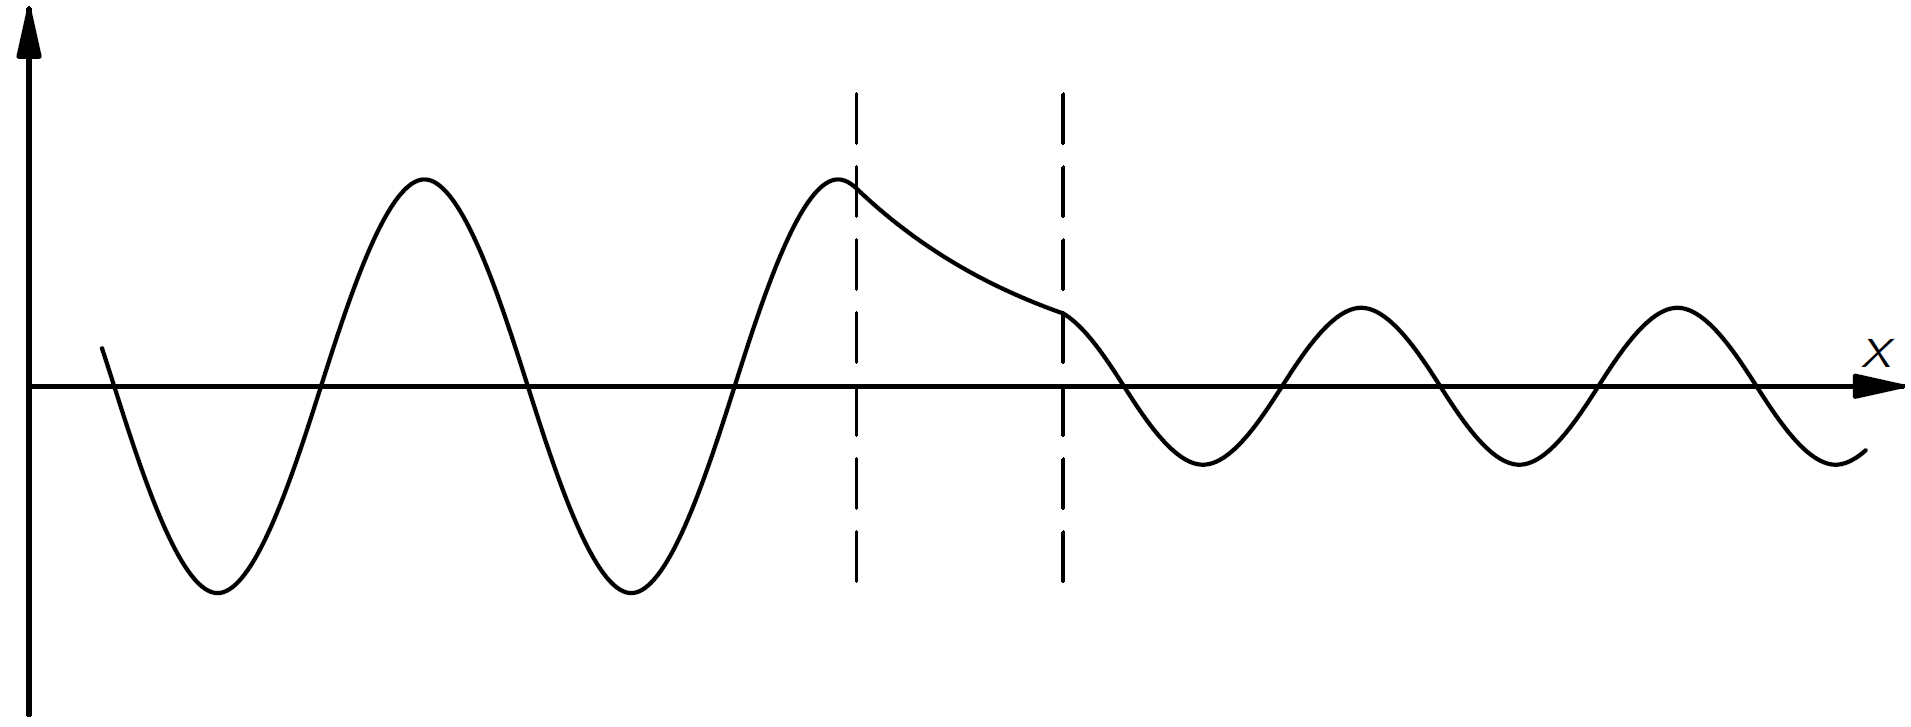
\includegraphics[width=0.6\textwidth]{immagini/tunneling_effect.png}
\end{figure}
\hspace{-0.6cm}Se abbiamo una barriera di tunneling, cioè una barriera in cui l'energia potenziale è maggiore dell'energia della particella, ci aspettiamo che la funzione d'onda penetri all'interno della barriera con un decadimento tipicamente esponenziale. Se la barriera è sufficientemente sottile, la funzione d'onda risulta non nulla anche dall'altro lato, rendendo possibile il tunneling.\\
Lo stesso tipo di descrizione può essere applicato anche al condensato superconduttivo. Possiamo quindi immaginare che la funzione d'onda collettiva del condensato abbia una probabilità non nulla di penetrare nella regione classicamente proibita rappresentata dalla barriera isolante. Questo processo avviene simmetricamente da entrambi i lati, poiché su entrambi i lati della barriera sono presenti superconduttori.\\
In questo senso possiamo interpretare la penetrazione della funzione d'onda macroscopica come un meccanismo di accoppiamento tra i due elettrodi. E, dato che stiamo parlando di un condensato, ciò implica che esiste una probabilità finita di trovare coppie di Cooper provenienti da un lato anche nell'altro lato della giunzione.\\
\mn{Per questa parte mi sono basato su \cite{Feynman}.}
Per descrivere questo effetto possiamo utilizzare una derivazione semplice dell'effetto Josephson, basata sull'idea di trattare il condensato come una funzione d'onda collettiva, ma formalmente descritta come una funzione d'onda a singola particella.\\
Chiamiamo $\psi_L$ l'ampiezza di probabilità di trovare un elettrone sul lato sinistro e $\psi_R$ quella corrispondente al lato destro. Nello stato superconduttivo, $\psi_L$ rappresenta la funzione d'onda collettiva di tutti gli elettroni del lato sinistro, mentre $\psi_R$ descrive analogamente il lato destro.\\
Le due ampiezze devono soddisfare le seguenti equazioni\mn{Le equazioni seguenti non sono altro che le equazioni di Schrödinger per le due funzioni d'onda. Il secondo termine nasce dal fatto che, se immaginiamo che la funzione d'onda superconduttiva possa penetrare attraverso la barriera, allora ciascun lato contiene anche una componente proveniente dall'altro lato.}:
\begin{equation*}
\begin{split}
    i\hbar \pdv{\psi_L}{t}
    &= U_1\psi_L + K\psi_R
    \\
    i\hbar \pdv{\psi_R}{t}
    &= U_2\psi_R + K\psi_L
\end{split}
\end{equation*}
La costante $K$ è una caratteristica della giunzione. Se $K=0$, queste due equazioni descriverebbero semplicemente gli stati fondamentali dei due superconduttori, con energie $U_1$ e $U_2$.\\
L'accoppiamento tra i due lati è invece descritto proprio dal termine proporzionale a $K$, che rappresenta la possibilità di una ``perdita'' di ampiezza di probabilità da un lato all'altro della barriera.\\
Se i due lati fossero identici, avremmo $U_1=U_2$ e potremmo semplicemente eliminare il termine energetico comune. Supponiamo però di collegare i due superconduttori ai terminali di una batteria, in modo da applicare una differenza di potenziale $V$ attraverso la giunzione. In questo caso $U_1-U_2=eV$. Possiamo allora scegliere convenientemente lo zero dell'energia a metà tra i due livelli energetici. Le equazioni diventano quindi:
\begin{equation*}
\begin{split}
    i\hbar \pdv{\psi_L}{t}
    &= \frac{eV}{2}\psi_L + K\psi_R
    \\[0.2cm]
    i\hbar \pdv{\psi_R}{t}
    &= -\frac{eV}{2}\psi_R + K\psi_L
\end{split}
\end{equation*}
Queste sono le equazioni standard di due stati quantistici accoppiati.\\
Per risolverle scriviamo $\psi_L$ e $\psi_R$ in termini di modulo e fase:
\begin{equation*}
    \psi_L
    =
    \sqrt{n_L}e^{i\phi_L}
    \qq{,}
    \psi_R
    =
    \sqrt{n_R}e^{i\phi_R}
\end{equation*}
dove $\phi_L$ e $\phi_R$ sono le fasi dei due superconduttori e $n_L$, $n_R$ rappresentano le densità elettroniche nei due lati della giunzione. In pratica queste densità sono quasi identiche e coincidono essenzialmente con la densità elettronica normale $n_0$ del materiale superconduttore.\\
Sostituendo queste espressioni nelle equazioni precedenti e separando parte reale e parte immaginaria, si ottengono quattro equazioni. Introducendo la differenza di fase $\varphi=\phi_R-\phi_L$, si trova:
\begin{equation}
    \begin{split}
        \dot{n}_L
        &=
        \frac{2}{\hbar}
        K\sqrt{n_Rn_L}
        \sin\varphi
        \\[0.2cm]
        \dot{n}_R
        &=
        -
        \frac{2}{\hbar}
        K\sqrt{n_Rn_L}
        \sin\varphi
    \end{split}
    \label{eq:derivate_densità}
\end{equation}
e
\begin{equation}
    \begin{split}
        \dot{\phi}_L
        &=
        -
        \frac{K}{\hbar}
        \sqrt{\frac{n_R}{n_L}}
        \cos\varphi
        -
        \frac{eV}{2\hbar}
        \\[0.2cm]
        \dot{\phi}_R
        &=
        -
        \frac{K}{\hbar}
        \sqrt{\frac{n_L}{n_R}}
        \cos\varphi
        +
        \frac{eV}{2\hbar}
    \end{split}
    \label{eq:derivate_fasi}
\end{equation}
Consideriamo dapprima le \eqrefcustom{eq:derivate_densità}. Esse mostrano che $\dot{n}_L=-\dot{n}_R$, come è naturale aspettarsi: gli elettroni passano da un lato all'altro, facendo aumentare la densità da un lato e diminuire quella dall'altro.\\
A questo punto si potrebbe osservare che $\dot{n}_L$ e $\dot{n}_R$ dovrebbero essere entrambi nulli se $n_L$ e $n_R$ sono costanti e pari a $n_0$. In realtà queste equazioni non raccontano tutta la fisica del problema. Esse descrivono infatti come le densità inizierebbero a variare se non esistessero forze elettriche aggiuntive dovute allo sbilanciamento tra il fluido elettronico e il background di ioni positivi.\\
Queste equazioni descrivono quindi il tipo di corrente che tenderebbe a instaurarsi. La corrente da sinistra verso destra sarebbe:
\begin{equation*}
    I_s
    =
    2e\mathcal{V}\dot{n}
    =
    2e\mathcal{V}
    \frac{2}{\hbar}
    Kn_0
    \sin\varphi,
\end{equation*}
dove $\mathcal{V}=Ad$ rappresenta il volume della giunzione.\\
Definendo la corrente critica della giunzione come
\begin{equation*}
    I_J
    =
    \frac{4e}{\hbar}
    Kn_0\mathcal{V}
\end{equation*}
la corrente può essere scritta nella forma
\begin{equation}
    I_s
    =
    I_J\sin\varphi.
    \label{eq:current_phase_relation}
\end{equation}
$I_J$ è un parametro caratteristico della giunzione e rappresenta chiaramente il valore massimo della supercorrente, ottenuto per differenze di fase pari a $\pi/2$ o suoi multipli.\\
Una corrente di questo tipo tenderebbe rapidamente a caricare il lato destro della giunzione, se non fosse che i due elettrodi sono collegati ai terminali della batteria. Le correnti provenienti dalla batteria compensano infatti questo trasferimento di carica, mantenendo costanti i potenziali e quindi anche le densità $n_L$ e $n_R$.\\
Le seconde equazioni, \eqrefcustom{eq:derivate_fasi}, descrivono invece l'evoluzione temporale delle fasi $\phi_L$ e $\phi_R$. A differenza delle precedenti, esse dipendono esplicitamente dalla tensione applicata.\\
Siamo interessati soprattutto alla differenza di fase $\varphi=\phi_R-\phi_L$, poiché è questa quantità che compare nella relazione corrente--fase. Sottraendo le due equazioni per $\dot{\phi}_L$ e $\dot{\phi}_R$ otteniamo:
\begin{equation}
    \dot{\varphi}=\frac{eV}{\hbar}
    \label{eq:phase_voltage_relation}
\end{equation}
Questa relazione mostra che, se è presente una differenza di potenziale, allora la differenza di fase tra i due superconduttori evolve nel tempo.\\
L'\eqrefcustom{eq:current_phase_relation} e l'\eqrefcustom{eq:phase_voltage_relation} sono le cosiddette \emph{relazioni di Josephson}. La prima descrive una corrente priva di dissipazione che attraversa la giunzione semplicemente a causa della differenza di fase tra i due superconduttori. La seconda mostra invece che, se la giunzione è inserita in un circuito con una tensione applicata, allora la differenza di fase evolve nel tempo.\\
Nel caso $V=0$, la differenza di fase resta costante e quindi anche la supercorrente rimane costante nel tempo. Se invece è presente una tensione costante $V=V_0\neq0$, allora la differenza di fase evolve linearmente:
\begin{equation*}
    \varphi(t)=\varphi(0)+\frac{2eV_0}{\hbar}t
\end{equation*}
Di conseguenza, anche la corrente diventa una funzione oscillante del tempo.\\
In pratica, però, tali oscillazioni sono estremamente rapide. Per questo motivo, sperimentalmente si parla ancora di effetto Josephson in corrente continua (DC Josephson effect), poiché ciò che viene effettivamente misurato è spesso la corrente mediata nel tempo, che risulta costante e inferiore alla supercorrente ideale che si avrebbe con fase perfettamente costante.\\
In precedenza abbiamo menzionato l'effetto Josephson parlando della rottura spontanea della simmetria di gauge. Abbiamo osservato che questa situazione è analoga alla transizione ferromagnetica: un materiale paramagnetico sviluppa spontaneamente una magnetizzazione lungo una direzione arbitraria, rompendo la simmetria del sistema.\\
Per rivelare la direzione della magnetizzazione non basta osservare un singolo campione isolato; è invece necessario mettere in interazione due materiali ferromagnetici, in modo che la loro interazione magnetica renda osservabile tale direzione privilegiata.\\
La stessa idea vale per la superconduttività. La rottura spontanea della simmetria di gauge implica che ciascun superconduttore possieda una fase macroscopica ben definita. Questa fase, però, diventa fisicamente osservabile soltanto quando mettiamo due superconduttori in contatto attraverso una giunzione Josephson.\\
In questo caso, la differenza tra le due fasi produce direttamente una supercorrente attraverso la giunzione. L'effetto Josephson rappresenta quindi anche una manifestazione sperimentale della rottura spontanea della simmetria di gauge nel superconduttore.
\subsection{Realizzazioni delle giunzioni Josephson}
Come realizziamo una giunzione Josephson?
\begin{figure}[H]
    \centering
    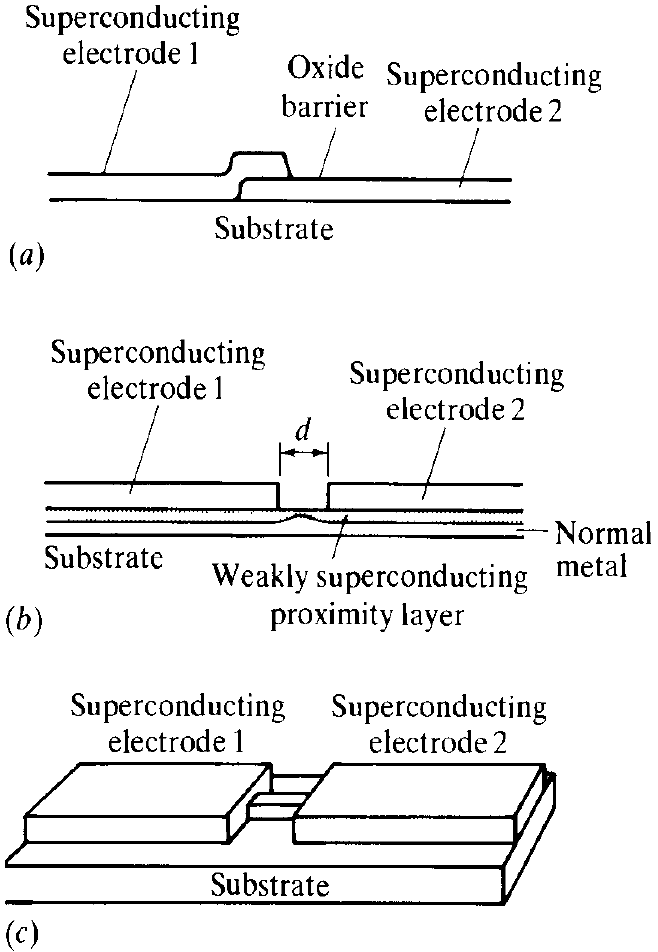
\includegraphics[width=0.5\textwidth]{immagini/Josephson_junction_realization.png}
\end{figure}
\hspace{-0.6cm}Quello che abbiamo menzionato finora è il caso (a), cioè il più semplice: uno strato di ossido cresciuto naturalmente tra due superconduttori, tipicamente in una struttura perpendicolare. Questa configurazione prende il nome di giunzione SIS (\textit{superconducting--insulating--superconducting}).\\
Esistono però anche altri modi per ottenere una giunzione Josephson. In particolare, possiamo avere effetto Josephson, cioè una supercorrente che fluisce, anche in assenza di un materiale isolante tra i due superconduttori.\\
Possiamo infatti realizzare una giunzione superconducting--normal--superconducting, come nel caso (b). In questo caso non abbiamo un materiale isolante, ma uno spazio tra i due superconduttori, depositati sopra un substrato che diventa debolmente superconduttivo attraverso il cosiddetto \emph{effetto di prossimità}.\\
L'effetto di prossimità consiste nel fatto che un materiale normale può acquisire proprietà superconduttive per il semplice fatto di trovarsi a contatto con un superconduttore; almeno una piccola regione del metallo normale diventa quindi anch'essa superconduttiva.\\
In questa configurazione, sui due lati è presente una funzione d'onda superconduttiva, e la possibilità di avere una supercorrente che attraversa la giunzione è legata proprio alla presenza dello strato sottostante che diventa debolmente superconduttivo. Ciò che accade è che le coppie di Cooper possono diffondere nel metallo prossimitizzato, dando origine a una supercorrente attraverso la giunzione.\\
Una situazione simile si verifica quando, al posto di un metallo normale prossimitizzato, abbiamo uno strato di grafene. Questo è il caso della giunzione Josephson planare, nella quale i due elettrodi superconduttivi sono separati da uno strato di grafene.
\begin{figure}[H]
    \centering
    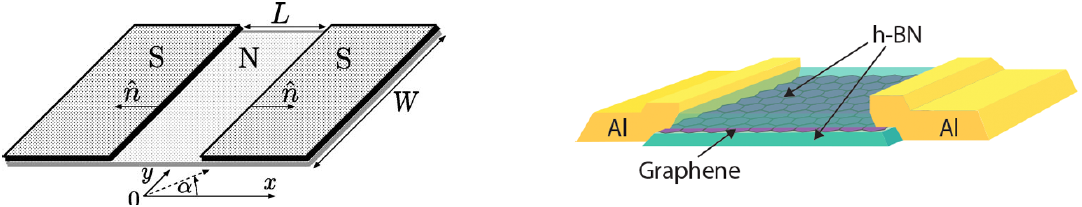
\includegraphics[width=0.8\textwidth]{immagini/graphene_Josephson_junction.png}
\end{figure}
\hspace{-0.6cm}Sperimentalmente il sistema appare come nella figura sopra. Lo strato di grafene è collegato ai lead superconduttivi e il contatto risulta quasi unidimensionale, poiché il grafene tocca gli elettrodi lungo una linea.\\
Inoltre il grafene deve essere sufficientemente isolato dall'ambiente; per questo motivo si utilizza spesso nitruro di boro esagonale (\textit{hexagonal boron nitride}, hBN), che presenta un eccellente accoppiamento strutturale con il grafene e introduce pochissime disomogeneità.\\
In definitiva, abbiamo un materiale normale oppure uno strato di grafene collegato a due superconduttori. Anche in questo caso otteniamo una giunzione Josephson, concettualmente non molto diversa dai casi precedenti.\\
Queste giunzioni Josephson presentano però una relazione corrente--fase che non coincide con la semplice dipendenza sinusoidale derivata in precedenza. Essa è rappresentata schematicamente nella figura seguente:
\begin{figure}[H]
    \centering
    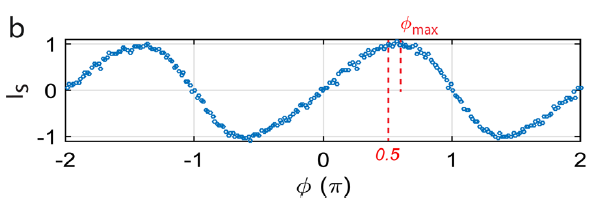
\includegraphics[width=0.6\textwidth]{immagini/current_phase_relation_graphene.png}
\end{figure}
\hspace{-0.6cm}La relazione rimane periodica, ma non è perfettamente sinusoidale e presenta una certa asimmetria. Inoltre, tale relazione corrente--fase può essere modulata tramite un gate: variando il potenziale di gate collegato ai due superconduttori, cambia infatti la forma della relazione corrente--fase.\\
Un'altra possibilità di ottenere l'effetto Josephson è il caso (c), detto \emph{weak link} oppure giunzione superconducting--constriction--superconducting.\\
In questo caso abbiamo un materiale interamente superconduttivo, ma con una strozzatura molto stretta tra le due regioni. Non è presente né uno strato isolante né uno spazio vuoto; tuttavia la regione di costrizione è così piccola da produrre un fenomeno analogo al tunneling, come se fosse presente una barriera isolante. Anche in questo caso compare quindi una corrente Josephson.\\
Abbiamo derivato in maniera fenomenologica le relazioni che caratterizzano la giunzione Josephson. Questa giunzione costituisce l'elemento circuitale fondamentale dei circuiti superconduttivi, oggi utilizzati in numerose applicazioni, ad esempio nei magnetometri.\\
Per studiare come l'effetto Josephson entri in gioco in circuiti contenenti giunzioni Josephson, si utilizza un modello elettrico in cui l'elemento superconduttivo viene interrotto dalla giunzione stessa.\\
Nei circuiti, la giunzione Josephson viene rappresentata convenzionalmente con una croce oppure con una croce racchiusa in un piccolo riquadro: questo è il simbolo circuitale della giunzione Josephson.\\
Per descrivere realisticamente questo elemento dobbiamo però considerare che la giunzione è costituita da due elettrodi posti uno di fronte all'altro e separati da uno strato isolante. Di conseguenza, i due elettrodi formano naturalmente anche un condensatore.\\
Per includere correttamente la giunzione all'interno di un circuito è quindi necessario tenere conto anche della capacità associata alla struttura.\\
Inoltre dobbiamo ricordare che non esiste soltanto il condensato superconduttivo. Finora abbiamo considerato soltanto lo stato fondamentale, cioè il condensato, ma sappiamo che esistono anche stati eccitati.\\
Questi stati eccitati diventano rilevanti a temperatura finita, quando possono verificarsi processi di tunneling a singola particella. In tali condizioni il comportamento della giunzione può diventare resistivo.\\
Quando il sistema entra in regime resistivo, il comportamento dipende dalla tensione applicata. Ricordiamo infatti che, nella caratteristica corrente--tensione di un superconduttore, non si osserva corrente fino al raggiungimento del gap $\Delta$; successivamente la corrente cresce e, per tensioni sufficientemente elevate, il sistema mostra un comportamento resistivo.\\
Questo significa che, per descrivere in generale una giunzione Josephson in un circuito, dobbiamo includere anche la possibilità di un canale resistivo che si attiva quando la tensione supera un certo valore. Si tratta quindi di una resistenza dipendente dalla tensione applicata.\\
Un modello circuitale che include tutti questi effetti è rappresentato schematicamente nella figura seguente:
\begin{figure}[H]
    \centering
    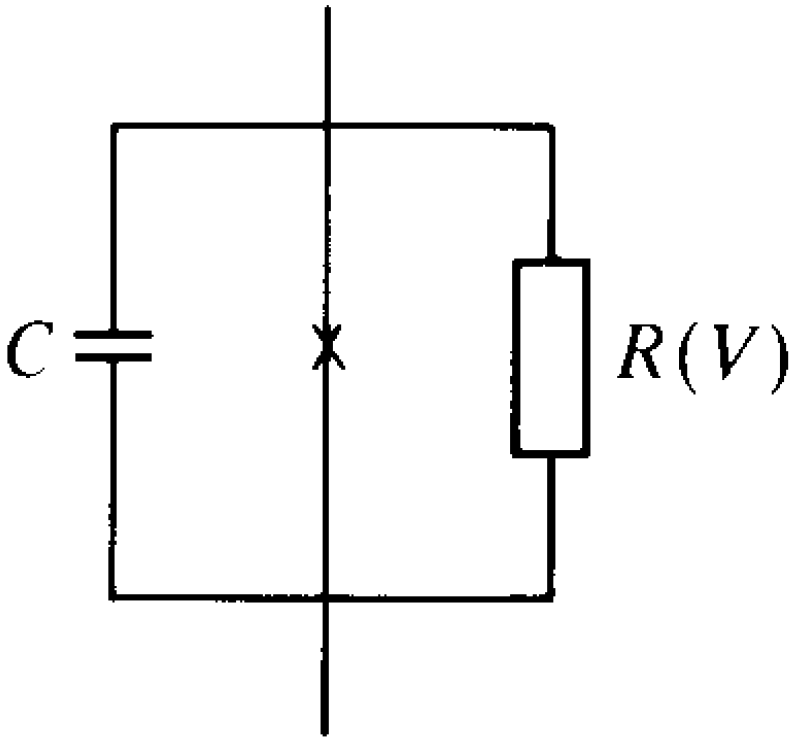
\includegraphics[width=0.3\textwidth]{immagini/RC_Josephson_junction.png}
\end{figure}
\hspace{-0.6cm}In questo modo si realizza il cosiddetto modello \emph{resistively and capacitively shunted Josephson junction} (RCSJ), cioè una giunzione Josephson con due shunt: uno capacitivo e uno resistivo.\\
Vedremo ora come questo elemento circuitale entra in gioco e come debba essere analizzato.
\subsection{Differenza di fase gauge-invariante e relazioni di Josephson in forma gauge-invariante}
Prima di passare oltre, consideriamo che cosa accade in presenza di un campo magnetico, poiché la descrizione sviluppata finora vale nel caso in cui il campo magnetico sia assente.\\
In presenza di un campo magnetico, dobbiamo scrivere relazioni gauge-invarianti. Sappiamo infatti che, se è presente un campo magnetico, dobbiamo effettuare una trasformazione di gauge, che implica una modifica del potenziale scalare e del potenziale vettore nel modo seguente:
\begin{equation*}
    \begin{dcases}
        V \to V - \frac{1}{c} \pdv{\Lambda}{t}
        \\[0.2cm]
        \vb{A} \to \vb{A} + \grad{\Lambda}
    \end{dcases}
\end{equation*}
Abbiamo inoltre visto che, affinché la teoria resti gauge-invariante, anche la funzione d'onda del condensato deve trasformarsi mediante un fattore di fase dipendente dalla carica e dalla funzione di gauge $\Lambda$:
\begin{equation*}
    \psi \to \psi e^{i \frac{2e}{\hbar c} \Lambda}
\end{equation*}
Questo implica che la densità di supercorrente assuma la forma
\begin{equation*}
    \vb{J}_s
    =n_s 2e \vb{v}_s
    =\frac{2e}{m}\qty(\hbar \grad{\varphi} - \frac{2e}{c}\vb{A}) \abs{\psi}^2
\end{equation*}
A partire da questa espressione possiamo definire la differenza di fase gauge-invariante $\gamma$ tra i due superconduttori:
\begin{equation*}
    \gamma
    =
    \int_{1}^{2}
    \grad{\varphi}\vdot d\vb{s}
    -
    \frac{2e}{\hbar c}
    \int_{1}^{2}
    \vb{A}\vdot d\vb{s}
\end{equation*}
dove gli estremi di integrazione indicano che l'integrale viene calcolato da un elettrodo all'altro della giunzione.\\
Il termine gauge-invariante è quindi composto da due contributi: il primo coincide con quello che compare in assenza di campo magnetico, mentre il secondo è l'integrale del potenziale vettore tra i due lati della giunzione.\\
Possiamo scrivere questa espressione in forma più compatta introducendo il quanto di flusso $\Phi_0=\frac{hc}{2e}$. Inoltre, integrando il primo termine, che è il gradiente della fase, otteniamo
\begin{equation*}
    \gamma
    =
    \Delta\varphi
    -
    \frac{2\pi}{\Phi_0}
    \int_{1}^{2}
    \vb{A}\vdot d\vb{s}
\end{equation*}
Questo significa che, se una giunzione Josephson è immersa in un campo magnetico, al posto della semplice differenza di fase $\Delta\varphi$ nell'argomento della funzione seno compare la differenza di fase gauge-invariante $\gamma$.\\
In altre parole, la differenza di fase effettiva non è più soltanto quella presente in assenza di campo magnetico, ma include anche un contributo legato al potenziale vettore e quindi al campo magnetico applicato.\\
Le relazioni di Josephson in forma gauge-invariante diventano quindi
\begin{equation*}
    I_s
    =I_J \sin{\gamma}
    \qq{,}
    \pdv{\Delta\varphi}{t}
    =\frac{2e}{\hbar}V
\end{equation*}
\subsection{Quantizzazione del flusso nella teoria BCS}
\textbf{Anello superconduttivo (come nella teoria GL)}\\
Vogliamo ora capire che cosa accade quando una giunzione viene inserita in un circuito e, in particolare, quando uno o due giunzioni interrompono un anello superconduttivo.\\
Già utilizzando la teoria di Ginzburg--Landau abbiamo derivato nel caso di un anello superconduttivo una relazione tra la supercorrente e il flusso del campo magnetico, ed è proprio in quel contesto che abbiamo introdotto il quanto di flusso. Vedremo ora che cosa accade quando l'anello superconduttivo viene interrotto da una o da due giunzioni Josephson, e vedremo che questo permette anche di identificare alcuni dispositivi fisici importanti.\\
Richiamiamo brevemente quanto già visto, riformulandolo però nel linguaggio della teoria BCS. Consideriamo un anello superconduttivo immerso in un campo magnetico applicato perpendicolarmente al piano dell'anello.
\begin{figure}[H]
    \centering
    
\begin{tikzpicture}
        \draw[gray!30!,line width=0.5cm] (0,0) circle (1.6cm);
        \draw (0,0) circle (0.4cm);
        \draw[rotate=45] (-0.4,0) -- (0.4,0);
        \draw[rotate=-45] (-0.4,0) -- (0.4,0);
    \end{tikzpicture}
\end{figure}
\hspace{-0.6cm}Sappiamo che lo stato fondamentale BCS può essere scritto nella forma
\begin{equation*}
    \Psi(\vb{r})
    =
    n_s(\vb{r}) e^{i \varphi(\vb{r})}
\end{equation*}
e che la densità di supercorrente gauge-invariante nell'anello è data da
\begin{equation*}
    \vb{J}_s
    \propto
    \grad{\varphi(\vb{r})}
    -
    \frac{2e}{\hbar c}\vb{A}(\vb{r}).
\end{equation*}
Ricordiamo che questa corrente, come avviene in ogni superconduttore, scorre soltanto in prossimità della superficie del materiale. A causa dell'effetto Meissner, infatti, nel bulk del superconduttore non è presente alcuna supercorrente.\\
Questo significa che, se invece di considerare la superficie guardiamo una linea chiusa sufficientemente interna al materiale, avremo
\[
\vb{J}_s=0.
\]
Di conseguenza, la combinazione presente nella parentesi deve annullarsi. Integrando lungo una linea chiusa interna al superconduttore otteniamo quindi
\begin{equation*}
    \oint
    \grad{\varphi}\vdot\dd{\vb{s}}
    =
    \frac{2e}{\hbar c}
    \oint
    \vb{A}\vdot\dd{\vb{s}}.
\end{equation*}
Consideriamo ora separatamente i due termini.\\
Per il primo termine, l'integrale del gradiente della fase lungo una linea chiusa è necessariamente un multiplo intero di $2\pi$, poiché la fase è una quantità periodica:
\begin{equation*}
    \oint
    \grad{\varphi}\vdot\dd{\vb{s}}
    =
    2\pi n.
\end{equation*}
Questo numero intero rappresenta il numero di avvolgimenti (\textit{winding number}) della fase lungo il percorso chiuso.\\
Per quanto riguarda invece l'integrale del potenziale vettore, dall'elettromagnetismo sappiamo che
\begin{equation*}
    \oint
    \vb{A}\vdot\dd{\vb{s}}
    =
    \int_{\Sigma}
    \vb{B}\vdot\dd{\vb{S}}
    =
    \Phi,
\end{equation*}
dove $\Phi$ è il flusso del campo magnetico attraverso la superficie $\Sigma$ delimitata dal contorno scelto.\\
Combinando le due relazioni otteniamo
\begin{equation*}
    2\pi n
    =
    \frac{2e}{\hbar c}\Phi.
\end{equation*}
Questa relazione implica la quantizzazione del flusso magnetico:
\begin{equation*}
    \Phi
    =
    n\Phi_0,
\end{equation*}
dove
\[
\Phi_0=\frac{hc}{2e}
\]
è il quanto di flusso.\\
Abbiamo già ottenuto questo risultato nella teoria di Ginzburg--Landau; qui lo stiamo semplicemente riformulando a partire dall'espressione della supercorrente in termini della fase del condensato BCS.\\
Questa relazione implica che, se prendiamo un anello metallico in presenza di un campo magnetico esterno e lo raffreddiamo al di sotto della temperatura critica, il campo magnetico viene espulso dal materiale a causa dell'effetto Meissner. Tuttavia, il flusso magnetico rimane intrappolato nell'anello in quantità discrete, multiple del quanto di flusso.\\
Questo flusso viene mantenuto dalla presenza di una supercorrente che circola lungo la superficie dell'anello.\\[0.2cm]
\textbf{Anello superconduttivo interrotto da una giunzione Josephson}\\
Supponiamo ora di interrompere l'anello mediante una giunzione Josephson.
\begin{figure}[H]
    \centering
    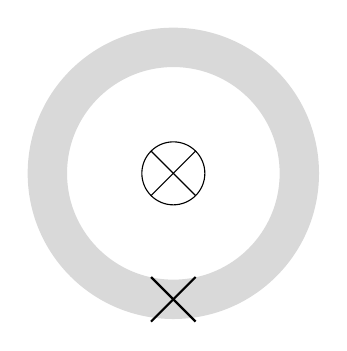
\begin{tikzpicture}
        \draw[gray!30!,line width=0.5cm] (0,0) circle (1.6cm);
        \draw (0,0) circle (0.4cm);
        \draw[rotate=45] (-0.4,0) -- (0.4,0);
        \draw[rotate=-45] (-0.4,0) -- (0.4,0);

        % giunzione
        \begin{scope}[shift={(0,-1.6)},rotate=90]
            \draw[thick, rotate=45] (-0.4,0) -- (0.4,0);
            \draw[thick, rotate=-45] (-0.4,0) -- (0.4,0);
        \end{scope}
    \end{tikzpicture}
\end{figure}
\hspace{-0.6cm}Tutto ciò che abbiamo detto finora continua a valere: in presenza di un campo magnetico la supercorrente deve essere gauge-invariante e, nel bulk del materiale superconduttivo, la corrente deve annullarsi. Quindi ancora una volta abbiamo $\vb{J}_s=0$.\\
La differenza rispetto al caso precedente è che ora il percorso chiuso non attraversa soltanto il superconduttore, ma contiene anche la giunzione Josephson. Di conseguenza, l'integrale del gradiente della fase lungo il contorno si separa in due contributi:
\begin{equation*}
    2\pi n
    =\oint \grad{\varphi}\vdot\dd{\vb{s}}
    =\int_{\text{sc}} \grad{\varphi}\vdot\dd{\vb{s}} + \int_{1}^{2} \grad{\varphi}\vdot\dd{\vb{s}}
\end{equation*}
Il secondo termine non è altro che la differenza di fase ai capi della giunzione, $\Delta\varphi = \phi_R-\phi_L$; il primo termine, essendo valutato all'interno del superconduttore, può invece essere espresso tramite il potenziale vettore:
\begin{equation*}
    \int_{\text{sc}}
    \grad{\varphi}\vdot\dd{\vb{s}}
    =
    \frac{2e}{\hbar c}
    \int_{\text{sc}}
    \vb{A}\vdot\dd{\vb{s}}.
\end{equation*}
Poiché il percorso differisce dal contorno chiuso completo soltanto nella piccola regione occupata dalla giunzione, possiamo approssimare questo integrale con quello sull'intero contorno chiuso.\mn{In pratica stiamo trascurando il contributo della giunzione.}
Otteniamo quindi
\begin{equation*}
    \frac{2e}{\hbar c}
    \int_{\text{sc}}
    \vb{A}\vdot\dd{\vb{s}}
    \approx
    \frac{2e}{\hbar c}\Phi
    =
    2\pi\frac{\Phi}{\Phi_0}
\end{equation*}
Complessivamente si ha quindi
\begin{equation*}
    2\pi n
    =
    \Delta\varphi
    +
    2\pi\frac{\Phi}{\Phi_0}
\end{equation*}
Scegliendo $n=0$,\mn{Il motivo di questa scelta è da chiarire meglio.} otteniamo
\begin{equation*}
    \Delta\varphi=-2\pi\frac{\Phi}{\Phi_0}
\end{equation*}
Questo significa che la differenza di fase ai capi della giunzione è direttamente proporzionale al flusso magnetico concatenato con l'anello.\\
Di conseguenza, se abbiamo una giunzione Josephson che interrompe un anello superconduttivo immerso in un campo magnetico, esiste una quantità osservabile macroscopicamente, cioè il flusso magnetico, direttamente proporzionale alla differenza di fase del condensato tra i due lati della giunzione.\\
In altre parole, la relazione precedente collega la differenza di fase della funzione d'onda superconduttiva — una quantità microscopica, profondamente legata alla natura dello stato superconduttivo e difficilmente osservabile direttamente — a una grandezza macroscopica facilmente misurabile, cioè il flusso magnetico attraverso l'anello, che può essere realizzato con dimensioni arbitrarie.
\subsection{Dispositivo a interferenza quantistica superconduttiva (SQUID)}
Se modifichiamo leggermente il circuito e, invece di avere una singola giunzione, introduciamo due giunzioni che interrompono il materiale superconduttivo, realizziamo quello che viene chiamato \emph{superconducting quantum interference device} (SQUID), cioè un dispositivo che permette di osservare l'interferenza quantistica tra le funzioni d'onda dei condensati superconduttivi nei due rami del circuito.\\
Facciamo attenzione al significato dell'espressione ``interferenza quantistica''. In meccanica quantistica siamo abituati a parlare di interferenza a partire dalle particelle elementari, poiché descriviamo gli elettroni tramite funzioni d'onda e consideriamo la loro sovrapposizione. Normalmente questo non ci sorprende troppo, perché stiamo parlando di sistemi microscopici.\\
Nel caso dello SQUID, invece, abbiamo un dispositivo che permette di osservare sperimentalmente l'interferenza tra funzioni d'onda di condensati macroscopici. Si tratta quindi di un effetto quantistico che coinvolge funzioni d'onda collettive di un condensato elettronico e che diventa direttamente osservabile attraverso correnti macroscopiche.\\
Vediamo ora come funziona il dispositivo.
\begin{figure}[H]
    \centering
    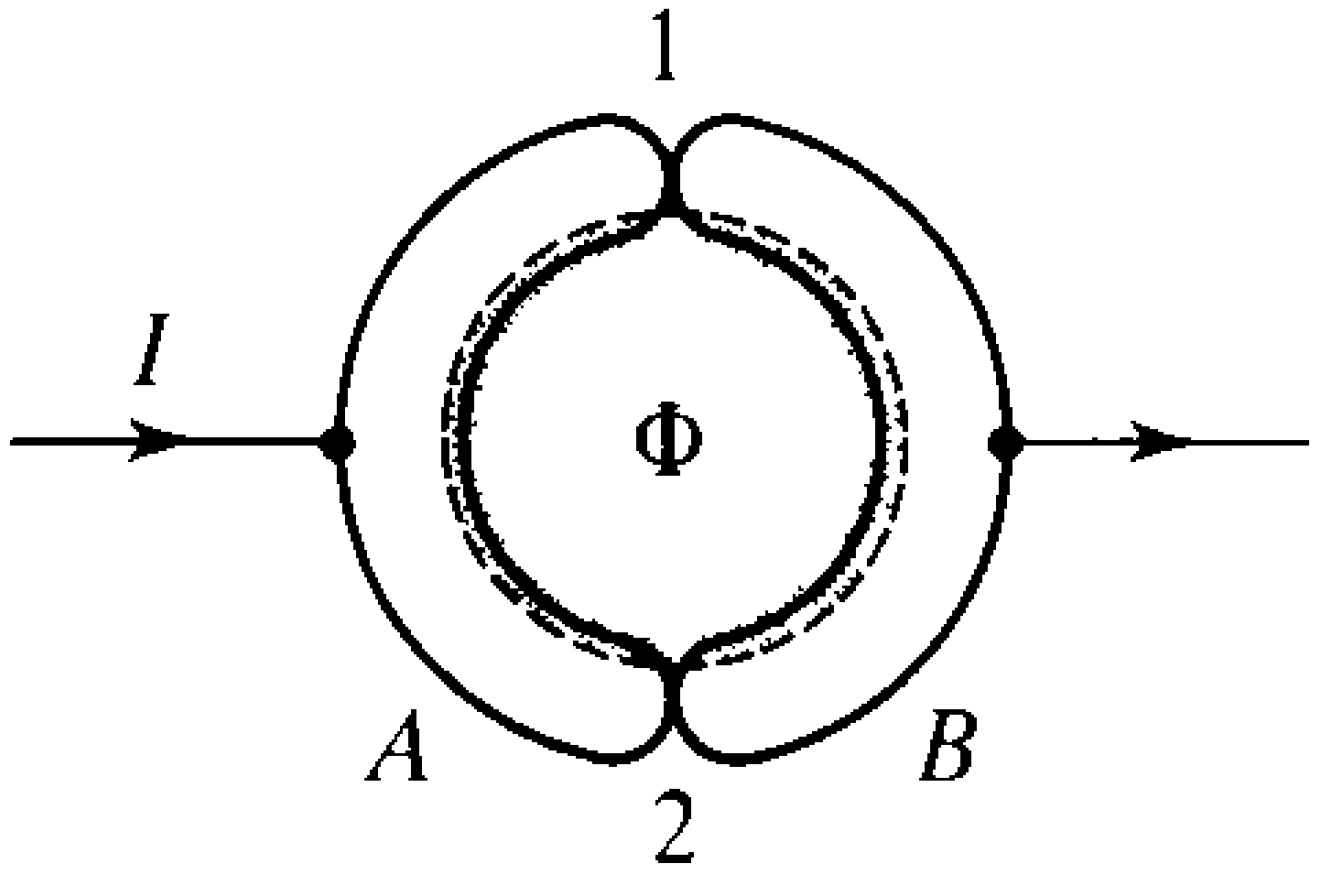
\includegraphics[width=0.45\textwidth]{immagini/SQUID.png}
\end{figure}
\hspace{-0.6cm}Possiamo eseguire per le due giunzioni la stessa derivazione fatta in precedenza nel caso di una singola giunzione. Possiamo quindi definire le due differenze di fase gauge-invarianti:
\begin{equation*}
    \begin{split}
        \gamma_1
        &=
        \Delta\varphi_1
        -
        \frac{2\pi}{\Phi_0}
        \int_{\text{link }1}
        \vb{A}\vdot\dd{\vb{s}}
        \\[0.2cm]
        \gamma_2
        &=
        \Delta\varphi_2
        -
        \frac{2\pi}{\Phi_0}
        \int_{\text{link }2}
        \vb{A}\vdot\dd{\vb{s}}.
    \end{split}
\end{equation*}
Sappiamo inoltre che l'integrale del gradiente della fase lungo un contorno chiuso , poiché questa deve essere una funzione a un sol valore, deve essere nullo a meno di multipli interi di $2\pi$. Possiamo separare tale integrale in un contributo sugli elettrodi e in due contributi corrispondenti alle due giunzioni:
\begin{equation*}
    \oint
    \grad{\varphi}\vdot\dd{\vb{s}}
    =
    \int_{\text{el}}
    \grad{\varphi}\vdot\dd{\vb{s}}
    +
    \int_{\text{link }1}
    \grad{\varphi}\vdot\dd{\vb{s}}
    +
    \int_{\text{link }2}
    \grad{\varphi}\vdot\dd{\vb{s}}.
\end{equation*}
Poiché\mn{Si presti attenzione che le fasi sono definite andando da sinistra verso destra. Se il cammino di integrazione è scelto in senso orario, nel tratto lungo la giunzione 2 ci si sta spostando da destra verso sinistra, il che comporto un segno negativo.}
\begin{equation*}
    \int_{\text{link }1} \grad{\varphi}\vdot\dd{\vb{s}}
    =\Delta\varphi_1
    \qq{,}
    \int_{\text{link }2} \grad{\varphi}\vdot\dd{\vb{s}}
    =-\Delta\varphi_2
\end{equation*}
otteniamo
\begin{equation}
    \Delta\varphi_1
    - \Delta\varphi_2
    + \int_{\text{el}} \grad{\varphi}\vdot\dd{\vb{s}}
    =0
    \quad (\text{mod }2\pi)
    \label{eq:phase_difference_squid}
\end{equation}
Se gli elettrodi sono sufficientemente spessi rispetto alla profondità di penetrazione di London, possiamo assumere che all'interno del bulk superconduttivo la supercorrente sia nulla: $\vb{J}_s = 0$. In questa regione vale quindi
\begin{equation*}
    \grad{\varphi}=\frac{2\pi}{\Phi_0}\vb{A}
\end{equation*}
Possiamo quindi scrivere
\begin{equation*}
    \int_{\text{el}} \grad{\varphi}\vdot\dd{\vb{s}}
    =\frac{2\pi}{\Phi_0}\int_{\text{el}} \vb{A}\vdot\dd{\vb{s}}
\end{equation*}
D'altra parte, possiamo scrivere\mn{Anche in questo passaggio, il termine relativo alla seconda giunzione ha il segno invertito a causa del verso di percorrenza.}
\begin{equation*}
    \begin{split}
        \frac{2\pi}{\Phi_0}\int_{\text{el}} \vb{A}\vdot\dd{\vb{s}}
        & =
        \frac{2\pi}{\Phi_0} \qty( \oint \vb{A}\vdot\dd{\vb{s}}
        - \int_{\text{link }1} \vb{A}\vdot\dd{\vb{s}}
        + \int_{\text{link }2} \vb{A}\vdot\dd{\vb{s}} )
        \\[0.2cm]
        & =
        2\pi \frac{\Phi}{\Phi_0} 
        + \frac{2\pi}{\Phi_0} \qty(
        - \int_{\text{link }1} \vb{A}\vdot\dd{\vb{s}}
        + \int_{\text{link }2} \vb{A}\vdot\dd{\vb{s}} )
    \end{split}
\end{equation*}
Possiamo allora scrivere l'\eqrefcustom{eq:phase_difference_squid}, raggruppando i termini in maniera opportuna, nella forma
\begin{equation*}
    \Delta\varphi_1
    - \int_{\text{link }1} \vb{A}\vdot\dd{\vb{s}}
    - \qty( \Delta\varphi_2 - \int_{\text{link }2} \vb{A}\vdot\dd{\vb{s}}
    )
    + 2\pi\frac{\Phi}{\Phi_0}=0
\end{equation*}
cioè\mn{Il segno meno deriva soltanto da una scelta di convenzione per il verso di percorrenza del contorno.}
\begin{equation*}
    \gamma_1 - \gamma_2=-\frac{2\pi\Phi}{\Phi_0}
\end{equation*}
Questa relazione mostra che la differenza relativa tra le due fasi gauge-invarianti è controllata direttamente dal flusso magnetico applicato.\\
Supponiamo ora che le due giunzioni siano identiche e abbiano la stessa corrente critica $I_c$. Se definiamo le correnti positive nei due rami nello stesso verso, le correnti Josephson attraverso le due giunzioni sono
\begin{equation*}
    I_1=I_c\sin\gamma_1
    \qq{,}
    I_2=I_c\sin\gamma_2
\end{equation*}
La corrente totale che attraversa lo SQUID è quindi
\begin{equation*}
    I
    =I_1+I_2
    =I_c\qty(\sin\gamma_1+\sin\gamma_2)
\end{equation*}
Usando l'identità trigonometrica
\begin{equation*}
    \sin a+\sin b
    =
    2\sin\qty(\frac{a+b}{2})
    \cos\qty(\frac{a-b}{2})
\end{equation*}
otteniamo
\begin{equation*}
    I
    =
    2I_c
    \sin\qty(\frac{\gamma_1+\gamma_2}{2})
    \cos\qty(\frac{\gamma_1-\gamma_2}{2}).
\end{equation*}
Usando ora il vincolo di flusso, $\frac{\gamma_1-\gamma_2}{2} = \pi\frac{\Phi}{\Phi_0}$, si trova
\begin{equation*}
    I
    =
    2I_c
    \cos\qty(\pi\frac{\Phi}{\Phi_0})
    \sin\qty(\frac{\gamma_1+\gamma_2}{2})
\end{equation*}
Questo significa che il sistema presenta ancora un effetto Josephson, nel senso che esiste una supercorrente che circola nell'anello, ma l'ampiezza massima della corrente dipende ora dal flusso magnetico applicato. In particolare, il dispositivo può sostenere al massimo una corrente pari a
\begin{equation*}
    I_{\max}(\Phi)
    =2I_c\abs{\cos\qty(\pi\frac{\Phi}{\Phi_0})}
\end{equation*}
Variando il campo magnetico esterno possiamo quindi modulare la supercorrente massima che attraversa il circuito, come mostrato nel grafico seguente:
\begin{figure}[H]
    \centering
    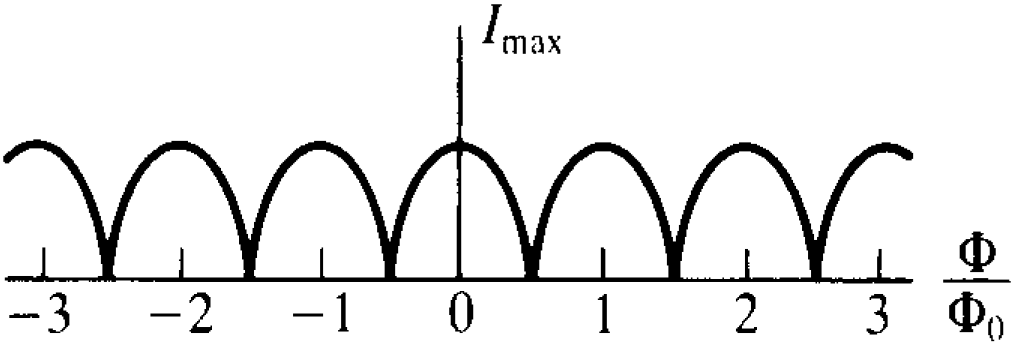
\includegraphics[width=0.6\textwidth]{immagini/SQUID_interference_pattern.png}
\end{figure}
\hspace{-0.6cm}Osserviamo una funzione oscillante, che rappresenta un vero e proprio pattern di interferenza, analogo a quello della doppia fenditura.\\
La differenza è che qui non stiamo osservando l'interferenza tra funzioni d'onda di singole particelle che attraversano due fenditure, ma l'interferenza tra le funzioni d'onda dei condensati superconduttivi che attraversano le due giunzioni Josephson. Le due giunzioni svolgono quindi il ruolo delle due fenditure.\\
Si tratta dunque di un pattern di interferenza di una funzione d'onda macroscopica, associata a un condensato formato da un numero macroscopico di elettroni descritti collettivamente da una singola funzione d'onda.\\
Questo fenomeno costituisce la base di magnetometri estremamente sensibili. Per capire il motivo, osserviamo con attenzione la regione del grafico in cui $\Phi/\Phi_0$ è prossimo a metà numero intero. Vediamo che piccolissime variazioni del campo magnetico applicato producono variazioni molto grandi della supercorrente. Di conseguenza, misurando la corrente superconduttiva possiamo ottenere informazioni estremamente precise su variazioni molto piccole del campo magnetico.\\
Facciamo attenzione al fatto che stiamo parlando di variazioni piccolissime della quantità $\Phi/\Phi_0$: questo significa che siamo in grado di rilevare variazioni di flusso magnetico confrontabili con una frazione del quanto di flusso.
\subsection{Fenomeni peculiari delle piccole giunzioni}
Finora abbiamo considerato l'effetto Josephson nel cosiddetto limite semiclassico, nel senso che la differenza di fase viene trattata come una variabile classica, pur avendo origine dalla meccanica quantistica. In questo contesto, quindi, la relazione di indeterminazione fase--numero che abbiamo già discusso per un superconduttore bulk non gioca alcun ruolo.\\
Quello che vedremo ora è che, se consideriamo giunzioni Josephson sufficientemente piccole, compare un comportamento in cui la natura di variabili coniugate di fase e numero diventa rilevante anche in un contesto quantistico. Ciò porterà a un effetto Josephson puramente quantistico.\\
Il punto è che oggi siamo in grado di realizzare elettrodi superconduttivi sufficientemente piccoli tali che la carica extra presente in queste piccole isole, anche a livello di singolo elettrone, diventi importante. In queste condizioni possiamo già intuire che la relazione di indeterminazione fase--numero, irrilevante nel caso di un superconduttore bulk, diventa invece significativa e conduce, come abbiamo detto, alla quantizzazione di fase e numero.\\
Vediamo innanzitutto quali siano le scale energetiche rilevanti e quali relazioni tra esse siano necessarie affinché emergano fenomeni quantistici. Consideriamo schematicamente un dispositivo del tipo seguente:
\begin{figure}[H]
    \centering
    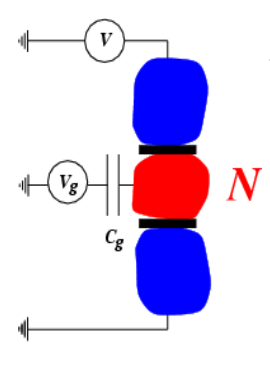
\includegraphics[width=0.27\textwidth]{immagini/single_electron_tunneling_geometry.png}
\end{figure}
\hspace{-0.6cm}Supponiamo di avere due elettrodi costituiti da metalli normali separati da uno strato isolante, per cui il dispositivo rappresentato è una giunzione NIN. Gli elettrodi sono generalmente collegati sia a un circuito di gate, che fissa il potenziale dell'isola centrale, sia a una tensione di trasporto.\\
In queste condizioni, poiché stiamo considerando elettrodi molto piccoli, tali elettrodi vengono spesso chiamati \emph{grains}. Questa è la tipica geometria di un dispositivo a tunneling di singolo elettrone. Abbiamo già discusso in passato che, anche nel caso di elettrodi normali, la presenza di due elettrodi affacciati implica un effetto capacitivo, per cui possiamo definire una capacità di giunzione, legata al costo elettrostatico associato alla presenza di cariche extra, ad esempio sull'isola centrale.\\
L'energia elettrostatica minima corrisponde naturalmente al caso in cui sia presente un elettrone aggiuntivo sull'isola. Tale configurazione comporta un costo energetico chiamato \emph{charging energy}:
\begin{equation*}
    E_C
    =
    \frac{e^2}{2C}
\end{equation*}
dove $C$ è la capacità della giunzione. Questa rappresenta una scala energetica fondamentale quando si considerano elettrodi di dimensioni ridotte.\\
Inoltre, per questo circuito possiamo definire anche una resistenza di tunneling, cioè una resistenza associata agli effetti dissipativi dovuti alla presenza dello strato isolante.\\
Per stimare quando gli effetti di carica diventano rilevanti, dobbiamo confrontare innanzitutto l'energia di carica con l'energia termica. La scala energetica delle fluttuazioni termiche è infatti $k_B T$. Per poter osservare effetti di carica dobbiamo quindi richiedere che si abbia
\begin{equation*}
    E_C > k_B T
\end{equation*}
Dobbiamo tenere presente che il nostro interesse è rivolto a elettrodi superconduttivi, quindi a temperature piuttosto basse. Ad esempio, a $T=1\;\rm K$, l'energia elettrostatica associata a un singolo elettrone risulta maggiore dell'energia termica purché la capacità sia minore di circa $10^{-15}\,\rm F$. Utilizzando l'espressione classica della capacità per una geometria piana, ciò corrisponde a un'area della giunzione inferiore a circa $10^{-8}\,\rm cm^2$.\\
Questo ci fornisce già un ordine di grandezza delle dimensioni necessarie affinché gli effetti di carica siano osservabili a temperature dell'ordine di pochi Kelvin, cioè proprio le temperature a cui si manifesta la superconduttività.\\
Oltre a ciò, stiamo considerando sistemi quantistici e sappiamo che, in generale, per sistemi quantomeccanici esiste una relazione di indeterminazione che collega l'incertezza in energia al tempo caratteristico del fenomeno. Se consideriamo l'incertezza associata all'energia di carica necessaria per osservare effetti quantistici, dobbiamo avere
\begin{equation*}
    \Delta E_C
    >
    \frac{\hbar}{\Delta t}
    \approx
    \frac{\hbar}{RC},
\end{equation*}
dove $\Delta t$ rappresenta la scala temporale tipica del circuito. In un sistema in cui avviene tunneling, tale tempo può essere stimato tramite il tempo caratteristico $RC$, con $C$ capacità della giunzione. Questo tempo rappresenta approssimativamente il tempo medio durante il quale un singolo elettrone rimane confinato sull'isola.\\
Se consideriamo un'incertezza energetica dell'ordine dell'energia di carica, dalla relazione di indeterminazione otteniamo allora una condizione sulla resistenza:
\begin{equation*}
    \Delta E
    \sim
    \frac{e^2}{2C}
    \implies
    R
    >
    \frac{2\hbar}{e^2}
    \equiv
    R_Q
    \sim
    6\;\rm k\Omega.
\end{equation*}
La resistenza deve quindi essere maggiore di una quantità chiamata \emph{quanto di resistenza}. Tale nome non significa che essa derivi direttamente da un effetto quantistico, ma che compare naturalmente applicando la relazione di indeterminazione energia--tempo all'energia di carica associata a un singolo elettrone. Questo è quindi il regime di condizioni che le giunzioni devono soddisfare affinché diventino osservabili effetti legati all'energia di carica di un singolo elettrone.
\subsection{Relazioni di indeterminazione fase--numero nelle giunzioni Josephson}
Quello che vogliamo capire ora è quando, in queste condizioni, diventano visibili anche gli effetti associati alla relazione di indeterminazione tra fase e numero. A questo scopo, riassumiamo innanzitutto ciò che sappiamo già per un superconduttore bulk.\\
Sappiamo che lo stato fondamentale di un superconduttore bulk ha la forma
\begin{equation*}
    \ket*{g_s}
    =
    \prod_{\vb{k}}
    \bigl(
        u_{\vb{k}}
        +
        \nu_{\vb{k}} Z_{\vb{k}}^{\dag}
    \bigr)
    \ket*{0}
\end{equation*}
Questa forma esplicita implica che la fase relativa tra componenti con differente numero di particelle è fissata. Possiamo vederlo nel modo seguente. Consideriamo lo stato
\begin{equation*}
    \ket*{\psi_{\phi}}
    =
    \prod_{\vb{k}}
    \bigl(
        u_{\vb{k}}
        +
        \nu_{\vb{k}} e^{i\phi} Z_{\vb{k}}^{\dag}
    \bigr)
    \ket*{0}
\end{equation*}
che differisce dal precedente per la presenza di un fattore di fase $e^{i\phi}$ associato alla creazione di ogni coppia di Cooper.\\
Abbiamo già visto che questo stato, che non possiede un numero fissato di particelle, può essere scritto come combinazione lineare di stati a numero fissato di particelle $\ket*{\psi_N}$:
\begin{equation*}
    \ket*{\psi_{\phi}}
    =
    \sum_N
    \lambda_N
    e^{i\phi N/2}
    \ket*{\psi_N}
\end{equation*}
Se associamo quindi una fase $\phi$ a ogni coppia di Cooper, decomponendo lo stato in una sovrapposizione di stati con diverso numero di coppie otteniamo, davanti a ciascuno stato $\ket*{\psi_N}$ con numero fissato di elettroni, un fattore di fase $e^{i\phi N/2}$.\\
Questa scrittura mostra immediatamente che, ogni volta che fissiamo una fase $\phi$, il numero di particelle diventa incerto, poiché per ciascun valore della fase abbiamo una sovrapposizione di stati con differente numero di particelle.\\
Abbiamo inoltre visto che, per estrarre da questa combinazione lineare la componente con un numero fissato di particelle, diciamo $N'$, dobbiamo rendere completamente incerta la fase. Questo significa considerare lo stato ottenuto moltiplicando $\ket*{\psi_{\phi}}$ per il fattore $e^{-i\phi N'/2}$ e integrando poi su tutti i valori della fase tra $0$ e $2\pi$:
\begin{equation*}
    \begin{split}
        \int_0^{2\pi}
        \dd{\phi}
        e^{-i\phi N'/2}
        \ket*{\psi_{\phi}}
        &=
        \int_0^{2\pi}
        \dd{\phi}
        \sum_N
        \lambda_N
        e^{i\phi N/2}
        e^{-i\phi N'/2}
        \ket*{\psi_N}
        \\[0.2cm]
        &=
        \sum_N
        \lambda_N
        2\pi
        \delta_{N,N'}
        \ket*{\psi_N}
        \\[0.2cm]
        &=
        2\pi
        \lambda_{N'}
        \ket*{\psi_{N'}}
    \end{split}
\end{equation*}
Questo è un modo per mostrare che, per estrarre dallo stato $\ket*{\psi_{\phi}}$ la componente con numero fissato di particelle $N'$, dobbiamo rendere completamente incerta la fase, cioè integrare su tutti i possibili valori di $\phi$.\\
Consideriamo ora in particolare la relazione
\begin{equation*}
    \int_0^{2\pi}
    \dd{\phi}
    e^{-i\phi N'/2}
    \ket*{\psi_{\phi}}
    =
    2\pi
    \lambda_{N'}
    \ket*{\psi_{N'}}
\end{equation*}
Questa espressione ricorda molto ciò che si fa in meccanica quantistica ordinaria quando, nella rappresentazione delle coordinate, integriamo su tutte le posizioni possibili un'onda piana con momento fissato $k$:
\begin{equation*}
    \int_{-\infty}^{\infty}
    \frac{\dd{x}}{2\pi}
    e^{-ikx}
    \ket*{x}
    =
    \ket*{k}
\end{equation*}
In quel caso, rendere completamente incerta la posizione permette di ottenere uno stato a momento fissato. Questo porta alla relazione di indeterminazione tra posizione e quantità di moto, oppure, equivalentemente, tra posizione e vettore d'onda:
\[
\Delta x \Delta k \sim \frac{1}{2}.
\]
In maniera del tutto analoga, la corrispondenza formale con la relazione appena ottenuta suggerisce una relazione di indeterminazione tra numero di particelle e fase:
\[
\Delta N \Delta\phi \sim 1.
\]
Questa è proprio la relazione di indeterminazione fase--numero che abbiamo già incontrato.\\
Nel caso di un superconduttore bulk, avere un numero non fissato di particelle non costituisce un problema, perché l'incertezza relativa sul numero di particelle, che scala come l'inverso della radice quadrata del numero medio di particelle, risulta estremamente piccola:
\begin{equation*}
    \frac{\delta N}{\bar{N}}
    \sim
    \frac{\sqrt{T_c/T_F}}{\sqrt{N}}
    \sim
    10^{-13}
\end{equation*}
Questo significa che, anche se lo stato fondamentale di un superconduttore bulk non possiede un numero esatto di particelle, ciò non ha conseguenze fisicamente rilevanti.\\
La situazione cambia quando consideriamo un piccolo pezzo di superconduttore. In questo caso, avere un differente numero di particelle significa avere una differente quantità di carica elettrica, e quindi una diversa energia elettrostatica. Di conseguenza, l'incertezza nel numero di particelle diventa fisicamente importante.\\
A questo punto possiamo spingerci oltre questa analogia tra fase e numero. Poiché la fase è una variabile periodica, se la interpretiamo come una coordinata, la variabile coniugata associata deve essere discreta, in modo del tutto analogo a quanto accade per il momento angolare.\\
Facciamo quindi un ulteriore passo introducendo una quantizzazione fenomenologica. Abbiamo infatti due variabili caratteristiche dello stato quantistico del sistema, e abbiamo trovato tra esse una relazione di indeterminazione. Decidiamo quindi di trattarle come variabili quantistiche e, come conseguenza della relazione di indeterminazione, introduciamo una relazione di commutazione canonica tra fase e numero:
\begin{equation*}
    [\hat{\phi},\hat{N}]
    =
    i
\end{equation*}
Se vogliamo scrivere questa relazione in forma più simile alla relazione di commutazione posizione--momento, dobbiamo moltiplicare per $\hbar$. Inoltre, per rendere esplicito il fatto che le cariche rilevanti sono le coppie di Cooper, definiamo l'operatore $\hat{Q}$ come numero di coppie di Cooper:
\begin{equation*}
    \qty[
        \frac{\hbar}{2}\hat{\phi},
        2\hat{Q}
    ]
    =
    i\hbar.
\end{equation*}
Una volta quantizzate fase e numero, possiamo dire che lo stato BCS, essendo caratterizzato da una fase ben definita, è un autostato dell'operatore fase.\\
Così come esistono autofunzioni della fase, esistono anche autofunzioni del numero, che diventano gli autostati naturali del sistema quando la configurazione superconduttiva considerata è dominata dagli effetti di carica. In altre parole, quando l'energia elettrostatica è la scala energetica dominante, gli autostati del sistema sono gli autostati dell'operatore carica.\\
Vogliamo ora avvicinarci gradualmente al caso di una giunzione Josephson. Consideriamo quindi due superconduttori bulk e immaginiamo di avvicinarli tra loro. Il sistema formato da questi due superconduttori tenderà a raggiungere una configurazione di minima energia.\mn{Nelle slide compare la frase: ``If two SC are brought close enough, the system tends to a lower energy configuration by tunneling (similar to a molecular bond).''}\\
Questa configurazione di minima energia deve tenere conto dei processi di tunneling elettronico da un lato all'altro della giunzione. Per descrivere lo stato complessivo dei due superconduttori dobbiamo quindi considerare la possibilità che alcuni elettroni siano passati da un lato all'altro, anche se non sappiamo quanti.\\
Possiamo allora scrivere lo stato generale dei due superconduttori vicini come una sovrapposizione degli stati $\ket*{\psi^L}$ e $\ket*{\psi^R}$ dei due elettrodi. In linea di principio, tali stati possono contenere differenti numeri di cariche trasferite da una parte all'altra.\\
Supponiamo che inizialmente entrambi i superconduttori contengano $N$ elettroni. Possiamo allora avere stati in cui un certo numero di elettroni, diciamo $q$, è tunnelato da un lato all'altro. Poiché non sappiamo quale sia il valore effettivo di $q$, dobbiamo considerare una sovrapposizione di tutti questi stati:
\begin{equation*}
    \ket*{\psi}
    =\sum_q a_q \ket*{\psi^L_{N+q}} \hspace{-0.17cm} \ket*{\psi^R_{N-q}}
\end{equation*}
Sappiamo già che questi numeri di particelle non sono fissati esattamente. Questo implica una certa incertezza sulla fase, anche se non così estrema come nel caso di numero completamente fissato.\\
Una volta scritto questo stato, dobbiamo tenere presente che, poiché i numeri di particelle non sono fissati, possono esistere fluttuazioni. Tali fluttuazioni si manifestano sui due lati della giunzione, e quindi avremo un'incertezza su $q$. Il fatto stesso che nello stato compaiano tutti i valori di $q$ equivale a dire che esiste un'incertezza sulla carica trasferita.\\
Ma una differenza di carica tra i due lati implica anche una differenza di energia elettrostatica. In altre parole, uno stato di questo tipo corrisponde a una configurazione in cui compare una carica sui due lati della giunzione, con il conseguente costo energetico associato.\\
Se immaginiamo matematicamente il limite in cui l'energia di carica $E_C$ tende a zero, è chiaro che, in assenza di costo elettrostatico, ciascun elettrodo superconduttivo resterà nello stato di minima energia, cioè in uno stato a fase fissata. In questo caso le due fasi sono semplicemente variabili classiche, esattamente come nella descrizione semiclassica sviluppata finora.\\
La presenza di un'energia di carica, cioè il fatto che esista un costo energetico associato a cariche extra sui due lati della giunzione, implica invece che il sistema cerchi di minimizzare tali cariche aggiuntive. Questo conduce a una relazione di indeterminazione e quindi a un comportamento quantistico della differenza di fase $\varphi$ tra i due elettrodi.\\
Queste fluttuazioni quantistiche della fase implicano che, quando consideriamo due superconduttori affacciati l'uno di fronte all'altro includendo il tunneling di carica e l'energia elettrostatica, la differenza di fase e lo sbilanciamento di carica tra i due lati soddisfano anch'essi una relazione di indeterminazione.\\
Possiamo allora imporre fenomenologicamente anche in questo caso una relazione di commutazione tra la differenza di fase e lo sbilanciamento di carica:
\begin{equation*}
    \qty[
        \hat{\varphi},
        \hat{n}
    ]
    =
    i,
\end{equation*}
dove
\begin{equation*}
    \hat{\varphi}=\hat{\phi}_2-\hat{\phi}_1
    \qq{e}
    \hat{n}=\frac{\hat{n}_2-\hat{n}_1}{2}
\end{equation*}
Quello che stiamo facendo, quindi, è passare gradualmente dalla relazione di indeterminazione fase--numero per un singolo superconduttore alla relazione di indeterminazione tra differenza di fase e sbilanciamento di carica in una giunzione Josephson.\\
Possiamo infine riscrivere questa relazione in forma analoga a quella già ottenuta:
\begin{equation*}
    \qty[ \frac{\hbar}{2}\hat{\varphi},2\hat{Q}]
    =i\hbar
\end{equation*}
\section{Descrizione circuitale}
\subsection{Descrizione circuitale (classica) riformulata in termini della fase}
A questo punto vogliamo considerare circuiti che includono una giunzione Josephson sufficientemente piccola affinché gli effetti di carica diventino rilevanti.\\
Innanzitutto scriveremo le equazioni circuitali. Se abbiamo una giunzione Josephson inserita in un circuito, dobbiamo infatti scrivere le equazioni del circuito, cioè le relazioni elettrodinamiche, tenendo conto della relazione non lineare caratteristica dell'elemento Josephson. Successivamente vedremo che cosa accade quando quantizziamo carica e differenza di fase, in particolare otterremo quindi un'equazione circuitale trattata quantisticamente.\\
Partiamo dalla descrizione circuitale classica, riformulandola però in termini della fase. In questo contesto dobbiamo considerare le due relazioni di Josephson come relazioni costitutive dell'elemento circuitale rappresentato dalla giunzione Josephson, che convenzionalmente viene indicata con una croce.\\
Le due relazioni di Josephson collegano la corrente attraverso la giunzione e la differenza di potenziale ai capi della giunzione con la differenza di fase:
\begin{equation*}
    I=I_0 \sin{\phi_{LR}}
    \qq{,}
    V=\frac{\hbar}{2e}\dot{\phi}_{LR}
\end{equation*}
Inseriamo ora questa giunzione Josephson all'interno di un circuito. Per descrivere il circuito dobbiamo scegliere una convenzione per orientare corrente e differenza di potenziale. Utilizziamo la stessa convenzione dell'elettromagnetismo classico, cioè assumiamo che la corrente sia positiva da sinistra verso destra quando il potenziale a sinistra è maggiore di quello a destra:
\begin{equation*}
    V=V_L-V_R>0
    \implies
    I^{\text{L}\to\text{R}}>0
\end{equation*}
In questo modo tutto resta coerente con la legge di Ohm e con la convenzione usuale per i circuiti resistivi.\\
Questo vale per una singola giunzione. In generale, però, la giunzione farà parte di un circuito chiuso. Tale circuito potrà contenere capacità, induttanze o altri elementi circuitali.\\
Abbiamo inoltre visto che, quando una giunzione interrompe un anello superconduttivo, esiste una relazione tra la differenza di fase ai capi della giunzione e il flusso magnetico concatenato con l'anello:
\begin{equation*}
    \Phi=\frac{\hbar}{2e}\varphi
\end{equation*}
Poiché l'effetto Josephson implica che una differenza di fase variabile nel tempo produca una tensione, mettendo insieme questa relazione con quella che lega la fase al flusso otteniamo la legge di Faraday--Neumann--Lenz:
\begin{equation*}
    V = \frac{\hbar}{2e}\dot{\phi}_{LR} \equiv \dot{\Phi}
\end{equation*}
Un ulteriore punto importante è che, in presenza di un campo magnetico esterno, dobbiamo utilizzare quantità gauge-invarianti, in particolare la differenza di fase gauge-invariante.\\
Abbiamo visto che la differenza di fase gauge-invariante tra i due elettrodi sinistro e destro è
\begin{equation*}
    \gamma_L-\gamma_R
    =
    \phi_L-\phi_R
    -
    \frac{2\pi}{\Phi_0}
    \int_L^R
    \vb{A}\vdot\dd{\vb{s}},
\end{equation*}
dove il secondo termine rappresenta il contributo del potenziale vettore lungo un percorso interno alla giunzione.\\
In questo caso il flusso magnetico risulta collegato alla differenza di fase gauge-invariante, e anche la corrente Josephson dipende da essa:
\begin{equation*}
    \Phi
    =
    \frac{\hbar\gamma_{LR}}{2e}
    \qq{,}
    I_J
    =
    I_0 \sin{\gamma_{LR}}
\end{equation*}
La tensione resta invece legata alla derivata temporale della fase, mentre la derivata temporale del flusso magnetico è collegata al rapporto tra carica e capacità:
\begin{equation*}
    V_{LR}
    =
    \frac{\hbar\dot{\phi}_{LR}}{2e}
    \qq{,}
    \dot{\Phi}
    =
    \frac{Q}{C}
    =
    \int
    \vb{E}\vdot\dd{\vb{s}}
\end{equation*}
Queste sono quindi le relazioni elettrodinamiche che collegano i diversi elementi circuitali.\\
Questo tipo di descrizione circuitale conduce naturalmente all'espressione dell'energia immagazzinata in un elemento Josephson. Vedremo infatti che essa può essere scritta in termini di una scala energetica chiamata energia Josephson, proporzionale alla corrente critica della giunzione, moltiplicata per un termine del tipo $1-\cos{\varphi}$, mentre la corrente dipende come $\sin{\varphi}$.\\
Per vedere come emerga questa struttura, consideriamo che l'energia associata alla giunzione Josephson può essere interpretata come il lavoro elettrico compiuto dalla corrente nel caricare la giunzione:
\begin{equation*}
    E
    =
    \int_0^{t'}
    \dd{t'}
    V(t')
    I_J(t').
\end{equation*}
Usando le relazioni di Josephson possiamo riscrivere l'integrale come
\begin{equation*}
    E
    =
    \int_0^{t'}
    \dd{t'}
    \frac{\hbar}{2e}
    \dot{\phi}_{LR}(t')
    I_0
    \sin{\phi_{LR}(t')}
\end{equation*}
Effettuando il cambio di variabile otteniamo
\begin{equation*}
    E
    =
    \frac{\hbar I_0}{2e}
    \int_{\varphi(0)}^{\varphi(t')}
    \dd{\varphi}
    \sin{\varphi}
    =
    E_J
    \bigl[
        1-\cos{\varphi(t')}
    \bigr],
\end{equation*}
dove abbiamo assunto $\varphi(0)=0$ e definito l'energia Josephson come
\begin{equation*}
    E_J=\frac{\hbar I_0}{2e}
\end{equation*}
Questa quantità rappresenta quindi semplicemente il lavoro elettrico necessario a caricare la giunzione.\\
Vediamo quindi che stiamo gradualmente identificando tutti gli elementi circuitali e le corrispondenti energie necessarie per descrivere circuiti contenenti giunzioni Josephson.\\
In particolare possiamo usare le usuali rappresentazioni circuitali, reinterpretandole in termini della differenza di fase e del flusso magnetico:
\begin{itemize}[leftmargin=0.5cm]
    \item Resistenza: $V=RI_R \quad\Rightarrow\quad I_R=\frac{\dot{\Phi}}{R}$
    \item Capacità:
    $
    Q=CV
    \quad\Rightarrow\quad
    I_C=\dot{Q}=C\ddot{\Phi}
    $
    \item Induttanza:
    $
    V=L\dot{I}_L
    \quad\Rightarrow\quad
    I_L
    =
    \frac{1}{L}
    \int_0^t
    \dd{t}\,V
    =
    \frac{\Phi}{L}.
    $
\end{itemize}
A questo punto possiamo fare un'ulteriore osservazione.
\begin{figure}[H]
    \centering
    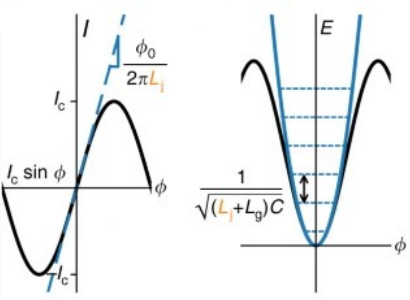
\includegraphics[width=0.5\textwidth]{immagini/josephson_energy_and_current.png}
\end{figure}
\hspace{-0.6cm}Abbiamo visto che l'energia Josephson è una funzione periodica che si annulla per $\varphi=0$. Se consideriamo il primo minimo della funzione, il potenziale appare approssimativamente parabolico nelle vicinanze del minimo stesso.\\
La corrente Josephson è anch'essa una funzione periodica che si annulla per $\varphi=0$, e per piccoli valori della fase è praticamente lineare:
\begin{equation*}
    I=I_J \sin{\varphi} \approx I_J \varphi
\end{equation*}
Analogamente, per piccoli valori di $\varphi$, possiamo approssimare l'energia come
\begin{equation*}
    E
    =E_J \bigl[ 1 - \cos{\varphi} \bigr]
    \approx E_J \qty[ 1 - \qty(1 - \frac{\varphi^2}{2}) ]
    =E_J\frac{\varphi^2}{2}
\end{equation*}
Quindi, per piccole oscillazioni della fase, il potenziale è approssimativamente armonico e la corrente dipende linearmente dalla fase.\\
In queste condizioni possiamo definire una induttanza equivalente della giunzione. Infatti:
\begin{equation*}
    I_J
    \approx
    I_0\varphi
    =
    I_0
    \frac{2e}{\hbar}
    \Phi.
\end{equation*}
Da questa relazione definiamo l'induttanza Josephson lineare:
\begin{equation*}
    L_{J,0}
    =
    \frac{\hbar}{2eI_0}
    =
    \frac{\Phi_0}{2\pi I_0}.
\end{equation*}
In generale, poiché la relazione corrente--fase non è lineare, anche l'induttanza sarà non lineare.\\
Allo stesso modo, dall'espressione dell'energia della giunzione possiamo definire una frequenza di oscillazione vicino al minimo del potenziale, detta frequenza di plasma Josephson. Essa dipende sia dall'induttanza sia dalla capacità della giunzione:
\begin{equation*}
    \omega_{p,0}
    =
    \frac{1}{\sqrt{L_{J,0}C}}
    =
    \sqrt{
        \frac{2\pi I_0}{C\Phi_0}
    }
\end{equation*}
La ragione per cui introduciamo tutte queste quantità è che esse permettono di identificare le scale energetiche caratteristiche della giunzione quando questa fa parte di un circuito.\\
Le due energie fondamentali sono:
\begin{itemize}[leftmargin=0.5cm]
    \item l'energia di carica, che ora scriviamo in termini della carica di una coppia di Cooper, e che rappresenta il costo elettrostatico associato al tunneling di due elettroni attraverso la giunzione;
    \item l'energia Josephson, cioè la scala energetica associata al termine Josephson dell'hamiltoniana.
\end{itemize}
Queste due energie si combinano nella frequenza di plasma:
\begin{equation*}
    \omega_{p,0}
    =
    \sqrt{2E_JE_C},
    \qquad
    E_C
    =
    \frac{(2e)^2}{2C},
    \qquad
    E_J
    =
    \frac{\hbar I_0}{2e}.
\end{equation*}
Vediamo quindi che:
\begin{itemize}[leftmargin=0.5cm]
    \item l'energia di carica dipende inversamente dalla capacità, quindi per giunzioni grandi $E_C$ è piccola;
    \item l'energia Josephson dipende invece dalla corrente critica e quindi dalle proprietà microscopiche della giunzione e dall'ampiezza di tunneling.
\end{itemize}
A seconda delle dimensioni e del materiale della giunzione possiamo quindi trovarci in due regimi distinti: $E_C \gg E_J$ oppure $E_J \gg E_C$.\\
Che cosa comportano questi due limiti per carica e fase? Per capirlo possiamo usare un'analogia con la meccanica quantistica di una particella soggetta a energia cinetica ed energia potenziale.\\
Se il termine dominante nell'hamiltoniana è il potenziale, gli autostati del sistema saranno autostati della coordinata. Se invece domina l'energia cinetica, gli autostati saranno onde piane, cioè autostati dell'impulso.\\
Le energie $E_C$ ed $E_J$ giocano un ruolo del tutto analogo:
\begin{itemize}[leftmargin=0.5cm]
    \item se domina l'energia di carica, gli autostati del sistema saranno stati a carica definita. La carica sarà quindi ben definita, mentre la fase sarà fortemente incerta;
    \item se domina l'energia Josephson, gli autostati saranno invece stati a fase ben definita, analogamente allo stato fondamentale BCS. In questo caso sarà la carica a diventare incerta.
\end{itemize}
Dobbiamo quindi interpretare queste due energie come l'analogo, rispettivamente, dell'energia cinetica e dell'energia potenziale, con la fase che gioca il ruolo della coordinata.\\
Abbiamo sviluppato tutte queste considerazioni perché ci serviranno per analizzare circuiti contenenti giunzioni Josephson in differenti regimi fisici.\\
Questi circuiti costituiscono infatti i mattoni fondamentali di molte applicazioni basate sulla superconduttività: dalla realizzazione di magnetometri estremamente sensibili fino, nel limite di dimensioni sempre più piccole, ai circuiti superconduttivi utilizzati come elementi base per il calcolo quantistico.
\subsection{Il modello RCSJ}
Il modello più semplice che consideriamo è quello di una giunzione Josephson reale. Una giunzione Josephson possiede infatti una capacità intrinseca, per cui dobbiamo includere nel modello una capacità in parallelo. Inoltre, abbiamo detto che anche in una giunzione Josephson ideale sono presenti impurità ed effetti dissipativi, dovuti ad esempio alla temperatura finita e alla presenza di quasiparticelle. Di conseguenza, dobbiamo considerare anche una componente resistiva in parallelo alla giunzione Josephson.\\
In modo qualitativo, maggiore è la resistenza, maggiore sarà la frazione di corrente che attraversa la giunzione Josephson, e viceversa. Per questo motivo possiamo modellizzare una giunzione Josephson reale come una giunzione ideale posta in parallelo con un condensatore e una resistenza:
\begin{figure}[H]
    \centering
    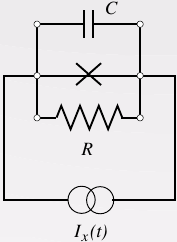
\includegraphics[width=0.3\textwidth]{immagini/RCSJ_model.png}
\end{figure}
\hspace{-0.6cm}Questo rappresenta quindi il blocco fondamentale costituito dalla giunzione Josephson ideale, dalla sua capacità e dagli effetti dissipativi.\\
In generale, la giunzione non è isolata, ma fa parte di un circuito. In particolare consideriamo il caso in cui il circuito sia polarizzato in corrente, cioè contenga un generatore di corrente.\\
Questo tipo di circuito prende il nome di modello RCSJ (\textit{Resistively and Capacitively Shunted Josephson Junction}).\\
L'equazione circuitale si scrive molto semplicemente osservando che la corrente di bias $I_x$, arrivando al nodo, si divide nei diversi rami:
\begin{equation}
    I_x=I_C + I_R + I_J
\end{equation}
Esprimiamo ora i vari contributi in termini delle grandezze circuitali e, in particolare, del flusso magnetico nel circuito:
\begin{equation}
    I_x
    =
    C \ddot{\Phi}
    +
    \frac{\dot{\Phi}}{R}
    +
    I_0
    \sin{
        \qty(
            \frac{2\pi\Phi}{\Phi_0}
        )
    }
    \label{eq:circuit_equation_RCSJ}
\end{equation}
Abbiamo ottenuto semplicemente un'equazione differenziale del secondo ordine che descrive il circuito contenente questi tre elementi.\\
Dimentichiamo ora momentaneamente il circuito e consideriamo invece una particella di coordinata $x$. L'equazione del moto di una particella soggetta a un potenziale e a dissipazione è
\begin{equation*}
    m\ddot{x}
    +
    \eta\dot{x}
    +
    U'(x)
    =
    0.
\end{equation*}
Notiamo che l'equazione circuitale \eqrefcustom{eq:circuit_equation_RCSJ} ha esattamente la stessa struttura: al posto della coordinata compare il flusso magnetico $\Phi$, il termine capacitivo gioca il ruolo dell'energia cinetica, il termine Josephson quello dell'energia potenziale, mentre la resistenza introduce dissipazione.\\
In altre parole, l'equazione del circuito è equivalente a quella di una particella di massa efficace proporzionale alla capacità, che si muove in un potenziale tale che
\begin{equation*}
    U'(\Phi)=I_0 \sin{ \qty( \frac{2\pi\Phi}{\Phi_0} )} - I_x
\end{equation*}
Integrando rispetto a $\Phi$, otteniamo il potenziale:
\begin{equation*}
    U(\Phi)=-E_J \cos{ \qty( \frac{2\pi\Phi}{\Phi_0} ) } - I_x\Phi
\end{equation*}
Vediamo quindi che il potenziale dipende dalla corrente di bias, che è un parametro controllabile esternamente, mentre l'energia Josephson e la capacità sono fissate una volta costruita la giunzione.\\
Vediamo ora come varia $U$ in funzione di $\Phi$:
\begin{figure}[H]
    \centering
    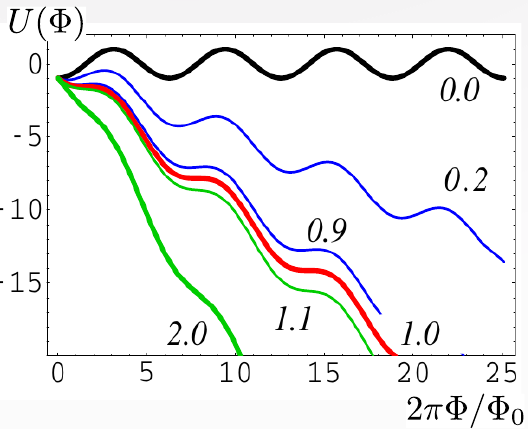
\includegraphics[width=0.55\textwidth]{immagini/potential_RCSJ.png}
\end{figure}
\hspace{-0.6cm}Le diverse curve corrispondono a differenti valori della corrente normalizzata $i_x=\frac{I_x}{I_0}$, cioè della corrente di bias in unità della corrente critica.\\
Consideriamo innanzitutto il caso $i_x=0$, cioè assenza di corrente di bias. In questo caso il potenziale coincide semplicemente con il potenziale sinusoidale Josephson.\\
Se invece la corrente di bias è diversa da zero, compare un termine lineare con segno negativo che inclina il potenziale. Il potenziale quindi non sarà più perfettamente periodico con la stessa ampiezza, ma risulterà progressivamente inclinato. Per piccoli valori della corrente di bias la forma resta simile a quella sinusoidale, ma compare una pendenza globale. All'aumentare della corrente di bias aumenta anche l'inclinazione del potenziale.\\
Finché $i_x\leq1$ il potenziale continua comunque a possedere minimi locali.\\
Questo si vede facilmente derivando il potenziale:
\begin{equation*}
    U'(\Phi)=0
    \quad\Longrightarrow\quad
    I_0 \sin{\qty(\frac{2\pi\Phi}{\Phi_0})}
    =I_x
\end{equation*}
cioè
\begin{equation*}
    \sin{\qty(\frac{2\pi\Phi}{\Phi_0})}
    =\frac{I_x}{I_0}
    =i_x
\end{equation*}
Questa equazione può avere soluzione soltanto per $i_x\leq1$. Ciò significa che il potenziale possiede minimi stabili soltanto quando la corrente di bias è minore o uguale alla corrente critica. Quando invece $i_x>1$, non esistono più minimi né massimi locali. Infatti, osservando ad esempio la curva corrispondente a $i_x=2$, vediamo che il potenziale risulta completamente inclinato.\\
Quello che vogliamo fare ora è capire qualitativamente come si comporta il circuito nei diversi regimi. Quando la corrente di bias è minore della corrente critica, il comportamento del circuito può essere compreso sfruttando l'analogia con una particella che si muove in un potenziale di questo tipo. Che cosa succede infatti a una particella soggetta a un potenziale come questo? Se la particella si trova in un minimo del potenziale, esistono due possibilità: o possiede energia sufficiente per superare la barriera, oppure non la possiede e quindi resta confinata nel minimo.\\
Naturalmente questa è ancora una descrizione classica. Nel nostro caso, una particella intrappolata in un minimo significa che il flusso magnetico resta costante, poiché la coordinata della particella resta fissa nel minimo del potenziale. Ma un flusso costante implica assenza di differenza di potenziale. Di conseguenza, il circuito presenta una corrente continua dovuta all'effetto Josephson, senza caduta di tensione: abbiamo cioè il classico effetto Josephson DC, ovvero una supercorrente finita in assenza di tensione.
\subsection{Tunneling quantistico macroscopico}
Prima di entrare nella derivazione dettagliata del comportamento del circuito nei diversi regimi (poiché abbiamo differenti scale energetiche e quindi differenti regimi dinamici), vediamo un'importante applicazione di questo tipo di circuito, introdotta originariamente per mettere in evidenza il cosiddetto \emph{tunneling quantistico macroscopico}.\\
Questo nome può sembrare quasi contraddittorio, perché normalmente associamo il tunneling quantistico a particelle microscopiche ed elementari, mentre gli oggetti macroscopici non mostrano in genere proprietà quantistiche osservabili. In questo caso, però, ciò che effettua il tunneling è la funzione d'onda collettiva di un enorme numero di elettroni, cioè il condensato superconduttivo stesso. Vedremo quindi come un circuito di questo tipo possa fornire evidenza sperimentale di tale fenomeno.\\
Consideriamo una versione semplificata del modello in cui trascuriamo gli effetti resistivi, che, come abbiamo detto, derivano da quasiparticelle, impurità, eccetera. Rimane quindi soltanto il comportamento puramente superconduttivo:
\begin{figure}[H]
    \centering
    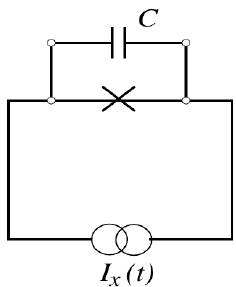
\includegraphics[width=0.35\textwidth]{immagini/CSJ_model.png}
\end{figure}
\hspace{-0.6cm}In questo caso otteniamo quella che viene chiamata \emph{capacitively shunted junction}. L'equazione circuitale si semplifica perché dobbiamo considerare soltanto la corrente attraverso la giunzione Josephson, la corrente di bias e quella che attraversa la capacità:
\begin{equation*}
    C \dv{V}{t}
    +
    I_c \sin{\varphi}
    =
    I_x(t)
\end{equation*}
Usando la seconda relazione di Josephson possiamo riscrivere il termine contenente la derivata della tensione come derivata seconda della fase:
\begin{equation*}
    C
    \frac{\hbar}{2e}
    \dv[2]{\varphi}{t}
    +
    I_c \sin{\varphi}
    =
    I_x(t)
\end{equation*}
Notiamo che, in questo caso, invece di scrivere l'equazione in funzione del flusso magnetico, la esprimiamo direttamente in termini della fase.\\
Moltiplicando entrambi i membri per $\frac{\hbar}{2e}$, otteniamo
\begin{equation*}
    C \qty( \frac{\hbar}{2e} )^2 \dv[2]{\varphi}{t} + \frac{\hbar}{2e} I_c \sin{\varphi} = \frac{\hbar}{2e} I_x(t)
\end{equation*}
Usando nuovamente l'analogia meccanica, questa equazione rappresenta il moto di una particella di coordinata $\varphi$ e massa efficace
\begin{equation*}
    m_{\rm eff}
    =
    C
    \qty(
        \frac{\hbar}{2e}
    )^2,
\end{equation*}
in un potenziale dato da
\begin{equation*}
    U(\varphi)
    = - \frac{\hbar}{2e} I_c \cos{\varphi} - \frac{\hbar}{2e} I_x \varphi
    = - E_J \cos{\varphi} - \frac{\hbar}{2e} I_x \varphi
\end{equation*}
Come nel caso precedente, il sistema è quindi equivalente a una particella che si muove in un potenziale che prende il nome di \emph{washboard potential}.\\
Facciamo ora un passo ulteriore: quantizziamo l'energia del sistema.\\
Abbiamo infatti una particella che si muove in questo potenziale; la coordinata è la fase $\varphi$, mentre la variabile coniugata è la carica. Poiché fase e carica soddisfano una relazione di indeterminazione, possiamo procedere alla quantizzazione del sistema e scrivere l'hamiltoniana quantistica associata.\\
Ricordiamo innanzitutto l'hamiltoniana classica di una particella:
\begin{equation*}
    H
    =
    \frac{p^2}{2m}
    +
    U(x),
\end{equation*}
che, una volta quantizzata, diventa
\begin{equation*}
    \hat{H}
    =
    \frac{\hat{p}^2}{2m}
    +
    U(\hat{x}).
\end{equation*}
Nel nostro caso il potenziale è $U(\varphi)$, che diventa quindi $U(\hat{\varphi})$, dove $\hat{\varphi}$ è l'operatore associato alla differenza di fase. Il termine cinetico è invece legato all'operatore carica, che è la variabile coniugata alla fase e gioca il ruolo dell'impulso.\\
Possiamo quindi scrivere l'hamiltoniana come
\begin{equation*}
    \hat{H}
    =
    \frac{\hat{Q}^2}{2C}
    +
    U(\hat{\varphi}).
\end{equation*}
Vediamo quindi che, attraverso questa quantizzazione fenomenologica, stiamo costruendo un'hamiltoniana che descrive un circuito elettrico contenente una giunzione Josephson. Questo è l'elemento concettualmente nuovo: quantizzare l'hamiltoniana di un circuito elettrico che include una giunzione Josephson.\\
Scriviamo ora esplicitamente i vari termini in funzione delle scale energetiche introdotte in precedenza. L'energia elettrostatica può essere espressa tramite l'energia di carica e l'operatore numero che conta le coppie di Cooper extra, mentre il termine potenziale è espresso in funzione dell'energia Josephson:
\begin{equation*}
    \hat{H}
    =
    E_C \hat{n}^2
    -
    E_J \cos{\hat{\varphi}}
    -
    \frac{\hbar}{2e}
    I_x
    \hat{\varphi}
\end{equation*}
A questo punto abbiamo tutti gli ingredienti necessari per comprendere qualitativamente ciò che accade. Consideriamo nuovamente il \emph{washboard potential}:
\begin{figure}[H]
    \centering
    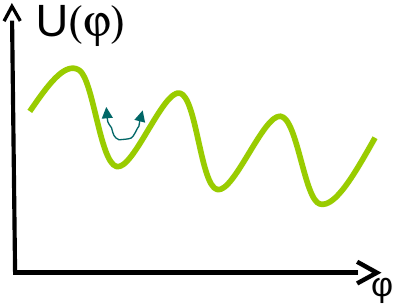
\includegraphics[width=0.4\textwidth]{immagini/washboard_potential.png}
\end{figure}
\hspace{-0.6cm}Se trattiamo il sistema come una particella quantistica di coordinata $\varphi$ in questo potenziale, sappiamo dalla meccanica quantistica che la particella non soltanto oscilla attorno a un minimo o supera classicamente la barriera se possiede energia sufficiente, ma può anche attraversare la barriera tramite tunneling quantistico.\\
Se quindi la particella non viene trattata classicamente, può effettuare tunneling tra minimi differenti del potenziale. Questo è consentito proprio perché stiamo trattando il circuito come un sistema quantistico.\\
A questo punto però dobbiamo chiederci: quale quantità fisica sta realmente effettuando il tunneling?\\
Ciò che attraversa la regione classicamente proibita è un numero macroscopico di particelle, cioè il condensato superconduttivo. In altre parole, si tratta del tunneling quantistico di un sistema macroscopico di elettroni. È proprio per questo motivo che il fenomeno prende il nome di \emph{tunneling quantistico macroscopico}.\\
Questo rappresenta il processo fisico profondo alla base dell'effetto Josephson.\\
Come possiamo osservare sperimentalmente tale fenomeno?\\
Se la particella si trova in un minimo del potenziale, il sistema si trova in uno stato a tensione nulla. Se però la particella effettua tunneling attraverso la barriera, una volta uscita dal minimo acquisisce tipicamente energia sufficiente per iniziare a ``scendere'' lungo il potenziale.\\
In termini dinamici, questo significa che la particella acquisisce una velocità non nulla, cioè una derivata temporale non nulla della fase:
\begin{equation*}
    \dot{\varphi}\neq0
\end{equation*}
Ma, per la relazione di Josephson, una variazione temporale della fase implica immediatamente la comparsa di una tensione ai capi della giunzione:
\begin{equation*}
    V
    =
    \frac{\hbar}{2e}
    \dot{\varphi}
\end{equation*}
Quindi, se il tunneling avviene, il valor medio della variabile quantistica $\hat{\varphi}$ cambia nel tempo e compare istantaneamente una tensione misurabile attraverso la giunzione.\\
Questo è precisamente il modo in cui viene rivelato sperimentalmente il tunneling quantistico macroscopico del condensato superconduttivo in un circuito di questo tipo.
\subsection{Osservabilità degli effetti quantistici nelle piccole giunzioni Josephson}
Commentiamo ora l'osservabilità di questi effetti quantistici.\\
Le energie che entrano in gioco sono quelle già discusse più volte: l'energia di carica, l'energia Josephson e la combinazione di queste due quantità che determina la frequenza di plasma.\\
Il comportamento della giunzione sarà essenzialmente classico, cioè caratterizzato semplicemente dal passaggio di corrente senza particolari effetti quantistici, quando gli effetti di carica sono trascurabili, cioè nel caso in cui $E_C \ll E_J$. In questo regime sappiamo che la carica è completamente indeterminata mentre la fase è ben definita, e si ottiene quindi il comportamento Josephson standard. Inoltre, la frequenza di plasma risulta molto più piccola dell'energia Josephson.\\
Gli effetti quantistici diventano invece rilevanti quando questa condizione non è più soddisfatta, cioè nel caso di giunzioni sufficientemente piccole, caratterizzate da capacità molto ridotte. Inoltre è necessario che la temperatura sia sufficientemente bassa, così da evitare la presenza di quasiparticelle eccitate che darebbero luogo a correnti dissipative.\\
Quello che serve quindi è avere un'energia di carica sufficientemente grande e, contemporaneamente, energie caratteristiche maggiori dell'energia termica.\\
Nella seguente tabella sono riportati gli ordini di grandezza tipici dell'area della giunzione, dell'energia Josephson, dell'energia di carica, della resistenza normale e della capacità per giunzioni realizzate in alluminio o niobio con barriera isolante realizzata con il relativo ossido.
\begin{table}[H]
    \centering
    \footnotesize
    \renewcommand{\arraystretch}{1.3}
    \begin{tabular}{|c|c|c|c|c|c|}
        \hline
        Giunzione & $A$ ($\mu$m$^2$) & $E_J$ ($\mu$eV) & $E_C$ ($\mu$eV) & $R_n$ ($\Omega$) & $C$ (pF) \\
        \hline
        Nb/NbO$_x$/PbIn & $10 \times 10$ & $2 \cdot 10^{4}$ & $5 \cdot 10^{-2}$ & $1.0$ & $\sim 10$ \\
        \hline
        Al/AlO$_x$/Al & $0.1 \times 0.1$ & $80.0$ & $470$ & $1000$ & $\sim 10^{-3}$ \\
        \hline
    \end{tabular}
    \caption*{
    Valori tipici dei parametri di giunzioni Josephson mesoscopiche in Nb ($J_c \approx 10\,\mathrm{A/cm^2}$) e di giunzioni ultrasmall in Al. In entrambi i casi la capacità specifica vale circa $c \approx 60\,\mathrm{fF/\mu m^2}$.}
\end{table}
\normalsize
\hspace{-0.6cm}La differenza principale tra questi due tipi di giunzioni è essenzialmente la loro dimensione. Le giunzioni in niobio sono tipicamente molto più grandi, con aree circa due ordini di grandezza maggiori rispetto alle giunzioni in alluminio.\\
Questo implica che:
\begin{itemize}[leftmargin=0.5cm]
    \item nelle grandi giunzioni l'energia di carica è molto piccola;
    \item nelle piccole giunzioni l'energia di carica diventa invece significativa;
    \item la capacità segue naturalmente l'andamento opposto.
\end{itemize}
Vi sono inoltre differenze anche nell'energia Josephson. Nel caso di giunzioni grandi (dove ``grande'' si riferisce all'area laterale, poiché lo spessore della barriera resta sempre dell'ordine di pochi nanometri affinché il tunneling sia possibile), la superficie dei superconduttori separati dalla barriera isolante è maggiore. Ciò implica un'ampiezza di tunneling più elevata e quindi un'energia Josephson maggiore.\\
In maniera qualitativa possiamo dire che, quanto più grande è la giunzione, tanto maggiore è la probabilità che un numero elevato di coppie di Cooper tunneli attraverso la barriera.\\
Ricapitoliamo ora ciò che abbiamo ottenuto finora. L'equazione circuitale del modello RCSJ, ottenuta semplicemente imponendo la conservazione della corrente, è
\begin{equation*}
    C \pdv{V}{t}
    +
    \frac{V}{R}
    +
    I_0 \sin{\varphi}
    =
    I_x.
\end{equation*}
Usando la seconda relazione di Josephson possiamo riscriverla nella forma
\begin{equation*}
    I_x
    =
    C \ddot{\Phi}
    +
    \frac{\dot{\Phi}}{R}
    +
    I_0
    \sin{
        \qty(
            \frac{2\pi\Phi}{\Phi_0}
        )
    }.
\end{equation*}
Abbiamo osservato che questa equazione è formalmente analoga a quella di una particella soggetta a dissipazione che si muove in un potenziale dato da
\begin{equation*}
    U(\Phi)
    = - \frac{\hbar}{2e} I_c \cos{\varphi} - \frac{\hbar}{2e} I_x \varphi
    = - E_J \cos{ \qty( \frac{2\pi\Phi}{\Phi_0} ) } - I_x\Phi
\end{equation*}
Il potenziale è quindi costituito da un termine cosinusoidale più un termine lineare dovuto alla corrente di bias. La sua forma è quella del cosiddetto \emph{washboard potential}, inclinato proprio dalla corrente di bias.\\
Abbiamo inoltre visto qualitativamente che il comportamento del sistema cambia radicalmente a seconda che $\frac{I_x}{I_c}<1$ oppure $\frac{I_x}{I_c} > 1$. Ricordiamo innanzitutto il primo caso. Se $\frac{I_x}{I_c}<1$, il potenziale possiede minimi locali, poiché imponendo la condizione di estremo $U'(\Phi)=0$ si ottengono soluzioni soltanto quando il termine sinusoidale può compensare la corrente di bias.\\
In questo caso il potenziale è il seguente:
\begin{figure}[H]
    \centering
    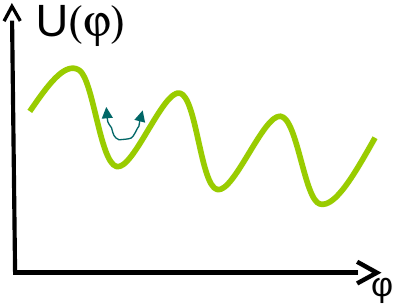
\includegraphics[width=0.4\textwidth]{immagini/washboard_potential.png}
\end{figure}
\hspace{-0.6cm}Interpretando il problema come quello di una particella in un potenziale, possiamo dire che la particella può rimanere confinata in uno dei minimi del potenziale, ottenendo così configurazioni stabili.\\
Se la particella si trova in un minimo con $\dot{\varphi}=0$, allora, per le relazioni di Josephson, non compare alcuna tensione e il sistema supporta una corrente priva di dissipazione.\\
Questa configurazione corrisponde al cosiddetto \emph{S-state}, cioè lo stato superconduttivo. Gli stati superconduttivi sono quindi configurazioni stabili del circuito che possono esistere soltanto se la corrente di bias è minore della corrente critica.\\
Per capire meglio la dinamica del sistema è utile studiare il comportamento del potenziale nelle vicinanze di un minimo $\varphi_m$. Sviluppando il coseno attorno a tale minimo otteniamo\mn{Questa cosa a me non convince per niente. Sviluppando in serie si dovrebbe ottenere
\begin{equation*}
    \cos{\varphi}
    \approx
    \cos{\varphi_m}
    -
    \frac{1}{2}
    \cos{\varphi_m}
    (\varphi-\varphi_m)^2
\end{equation*}
quindi comparirebbe un fattore $\cos{\varphi_m}$ che qui non appare. L'unica possibilità è che ci si stia mettendo nel limite di bias piccolo, cioè $I_x \ll I_c$, nel quale $\varphi_m \approx 2\pi m$ e quindi $\cos{\varphi_m}\approx1$.}
\begin{equation*}
    -E_J\cos{\varphi}
    \approx
    -E_J\cos{\varphi_m}
    +
    \frac{E_J}{2}
    (\varphi-\varphi_m)^2
\end{equation*}
Il potenziale risulta quindi approssimativamente parabolico nelle vicinanze del minimo. Il coefficiente del termine quadratico determina la frequenza delle piccole oscillazioni attorno al minimo, cioè la frequenza di plasma.\\
Come avviene per una particella ordinaria, tale frequenza dipende dalla massa efficace, che in questo caso è interpretata dalla capacità:
\begin{equation*}
    E_J
    =
    m\omega_p^2
    =
    C
    \qty(
        \frac{\hbar}{2e}
    )^2
    \omega_p^2
\end{equation*}
da cui
\begin{equation*}
    \omega_p
    =
    \sqrt{
        \frac{E_J}{C}
        \qty(
            \frac{2e}{\hbar}
        )^2
    }
    =
    \frac{\sqrt{2E_JE_C}}{\hbar}
\end{equation*}
Possiamo quindi interpretare la dinamica della giunzione, trascurando la dissipazione, come quella di una particella con energia fissata composta da contributi cinetici e potenziali.\\
Se la particella possiede energia sufficiente, può superare la barriera del potenziale e iniziare a ``rotolare'' lungo il washboard potential. In assenza di dissipazione questo moto persisterebbe indefinitamente; introducendo la resistenza, esso viene invece smorzato.\\
Vediamo ora che cosa accade quando la corrente di bias supera la corrente critica:
\begin{figure}[H]
    \centering
    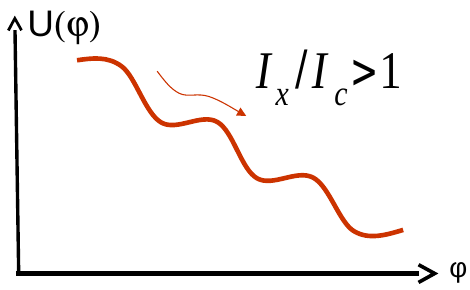
\includegraphics[width=0.4\textwidth]{immagini/washboard_potential_no_minima.png}
\end{figure}
\hspace{-0.6cm}In questo caso il potenziale non presenta più minimi, ma soltanto punti di flesso. Non esistono quindi configurazioni stabili e la condizione $\dot{\varphi}=0$ non può più essere soddisfatta.\\
Questo significa che compare necessariamente una tensione ai capi della giunzione. Inoltre, poiché nel circuito è presente una resistenza, la tensione genera anche una corrente dissipativa.\\
Per questo motivo, quando $I_x>I_c$, il sistema si trova nel cosiddetto \emph{R-state}, cioè nello stato resistivo, in contrapposizione allo stato superconduttivo.
\subsection{Caratteristica corrente--tensione}
Vogliamo adesso risolvere questa equazione nei due diversi regimi.\\
Cominciamo dal regime overdamped, cioè il regime in cui il fattore di qualità del circuito è minore di uno. Con fattore di qualità intendiamo la combinazione tra la frequenza di plasma delle oscillazioni attorno al minimo e la scala temporale del circuito determinata da $RC$,\mn{In altre parole, esso rappresenta il rapporto tra la scala temporale caratteristica del circuito la scala temporale delle oscillazioni attorno al minimo.} dal momento che stiamo considerando un circuito con comportamento sia resistivo che capacitivo.\\
Partiamo dall'equazione circuitale scritta in termini della fase:
\begin{equation*}
    I_x = C \frac{\hbar}{2e} \dv[2]{\varphi}{t} + \frac{\hbar}{2e} \frac{1}{R} \dv{\varphi}{t} + I_0 \sin{\varphi}
\end{equation*}
Dividendo per $I_c$ e ricordando che $\omega_p$ è data da
\begin{equation*}
    \omega_p=\qty(\frac{2eI_c}{\hbar C})^{\frac{1}{2}}
\end{equation*}
possiamo riscrivere tale equazione come
\begin{equation*}
    i_x = \frac{1}{\omega_p^2} \dv[2]{\varphi}{t} + \frac{1}{\omega^2_p} \frac{1}{R C} \dv{\varphi}{t} + \sin{\varphi}
\end{equation*}
Se adesso riscriviamo l'equazione in termini della quantità adimensionale $\tau=\omega_p t$, da cui $\dd{\tau}=\omega_p \dd{t}$ e $\dd[2]{\tau}=\omega_p^2 \dd[2]{\varphi}{t}$, otteniamo:
\begin{equation*}
    i_x = \dv[2]{\varphi}{\tau} + \frac{1}{Q} \dv{\varphi}{\tau} + \sin{\varphi}
\end{equation*}
dove
\begin{equation*}
    Q=\omega_p RC
\end{equation*}
è il fattore di qualità.\\
Se $Q \ll 1$, cioè se ci troviamo nel cosiddetto regime overdamped, il termine dissipativo domina rispetto alla derivata seconda della fase. Per capire quindi il comportamento del sistema possiamo limitarci all'equazione approssimata
\begin{equation*}
    i_x \approx \frac{1}{Q} \dv{\varphi}{\tau} + \sin{\varphi}
\end{equation*}
Questa equazione riproduce immediatamente il comportamento atteso per $I_x < I_c$, cioè la presenza di minimi del potenziale e quindi di stati stazionari.\sn{Infatti, per $I_x < I_c$ l'equazione ammette soluzioni statiche, nelle quali la fase assume un valore costante. Nel linguaggio del washboard potential ciò significa che esistono minimi del potenziale in cui la particella può fermarsi. In altre parole, se la corrente applicata è minore della corrente critica, la forza esercitata dalla corrente non è sufficiente a far "scivolare" la fase lungo il potenziale. La fase rimane intrappolata in un minimo e il sistema raggiunge un equilibrio stabile.}\\
A questo punto vogliamo trovare la relazione tra la corrente di bias applicata $I_x$ e la corrente che attraversa il circuito, espressa in forma adimensionale come $i=\frac{I}{I_c}$. Vogliamo inoltre derivare separatamente i contributi di corrente che attraversano la giunzione Josephson e la resistenza.\\
Nel regime $I_x<I_c$, la corrente scorre unicamente attraverso l'elemento Josephson e dipende dal valore della fase associato a uno dei minimi del potenziale. La dipendenza rispetto a $I_x$ risulta lineare: $i_J=i_x$\\
Nel grafico seguente dobbiamo quindi guardare soltanto la regione con $I_x<I_c$; la parte restante emergerà invece dal regime con $I_x>I_c$.
\begin{figure}[H]
    \centering
    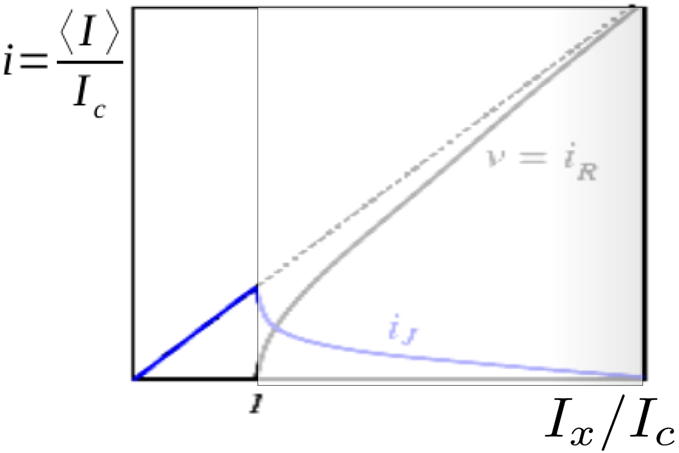
\includegraphics[width=0.5\textwidth]{immagini/IV_characteristic_RCSJ.png}
\end{figure}
\hspace{-0.6cm}Per trovare l'andamento per $I_x>I_c$, dobbiamo risolvere l'equazione. Riscriviamola come\sn{\cite{Tinkham} Se guardiamo la forma dell'equazione circuitale si vede che, per $I > I_{c}$, $\dv*{\varphi}{t}$ è sempre positivo, ma varia periodicamente con $\sin{\varphi}$. La fase avanza più lentamente (corrispondendo a una tensione istantanea più bassa) quando $\sin\varphi$ è positivo (così che la supercorrente sia nella direzione diretta), e viceversa quando $\sin\varphi$ è negativo e la supercorrente si oppone alla corrente continua di bias.}
\begin{equation*}
    \dv{\varphi}{\tau} = Q \qty( i_x-\sin{\varphi} )
\end{equation*}
Separando le variabili otteniamo
\begin{equation*}
    Q \dd{\tau} = \frac{\dd{\varphi}}{i_x-\sin{\varphi}}
\end{equation*}
Per trovare la tensione media temporale integriamo tale equazione per determinare il periodo di tempo $T$ richiesto affinché $\varphi$ aumenti di $2\pi$:
\begin{equation*}
    Q \int_{0}^{\tilde{T}} \dd{\tau} = \int_{0}^{2\pi} \frac{\dd{\varphi}}{i_x-\sin{\varphi}}
\end{equation*}
dove $\tilde{T}$ è il periodo in unità di $\omega_p$, quindi $\tilde{T}=\omega_p T$.\\
Si trova quindi\mn{Da notare che abbiamo usato il risultato noto
\begin{equation*}
    \int_{0}^{2\pi} \frac{\dd{\varphi}}{a-\sin{\varphi}}
    =
    \frac{2\pi}{\sqrt{a^2-1}}
    \quad\text{per } a>1
\end{equation*}}
\begin{equation*}
    Q\tilde{T} = \frac{2\pi}{\sqrt{i_x^2-1}}
\end{equation*}
Usando la definizione di $Q$, possiamo riscrivere questa relazione nella forma
\begin{equation*}
    \omega_p RC\,\tilde{T}
    =
    \frac{2\pi}{\sqrt{i_x^2-1}}
\end{equation*}
Invertendo la relazione otteniamo l'espressione del periodo delle oscillazioni:
\begin{equation}
    \tilde{T}
    =
    \frac{1}{\omega_p RC}
    \frac{2\pi}{\sqrt{i_x^2-1}}
    \label{eq:period_oscillations_RCSJ}
\end{equation}
Per procedere nello studio della corrente utilizziamo ora la seconda relazione di Josephson.\\
Nel limite overdamped la fase dipende dal tempo. Vogliamo quindi determinare il valor medio della fase e della corrente nei diversi elementi del circuito su un periodo caratteristico $\tilde{T}$.\\
Usiamo la relazione di Josephson
\begin{equation*}
    V
    =
    \frac{\hbar}{2e}
    \dot{\varphi}
\end{equation*}
e valutiamo il valor medio della tensione:
\begin{equation*}
    \expval*{V}
    = \frac{1}{\tilde{T}} \int_{0}^{\tilde{T}} V \dd{t}
    = \frac{\hbar}{2e} \frac{1}{\tilde{T}} \int_{0}^{\tilde{T}} \dd{t} \dot{\varphi}
    = \frac{\hbar}{2e} \expval*{\dot{\varphi}}
\end{equation*}
Quindi
\begin{equation*}
    \expval*{V} = \frac{\hbar}{2e} \expval*{\dot{\varphi}}
\end{equation*}
Se definiamo $\tilde{T}$ come il tempo necessario affinché la fase cambi di $2\pi$, possiamo approssimare
\[
\expval*{\dot{\varphi}}
\simeq
\frac{2\pi}{\tilde{T}},
\]
da cui
\begin{equation}
    \expval*{V}
    =
    \frac{\hbar}{e}
    \frac{\pi}{\tilde{T}}
    \label{eq:average_voltage_RCSJ}
\end{equation}
Sostituendo ora l'\eqrefcustom{eq:period_oscillations_RCSJ} nell'\eqrefcustom{eq:average_voltage_RCSJ} otteniamo
\begin{equation*}
    \expval*{V}=R\sqrt{I_x^2-I_c^2}
\end{equation*}
La corrente che attraversa la resistenza è quindi
\begin{equation*}
    I_R
    =\frac{\expval*{V}}{R}
    =\sqrt{I_x^2-I_c^2}
\end{equation*}
Usando infine la conservazione della corrente possiamo ricavare il valor medio della corrente Josephson:
\begin{equation*}
    \expval*{I_J}
    =I_c \expval*{\sin{\varphi}}
    =I_x-\sqrt{I_x^2 - I_c^2}
\end{equation*}
Osserviamo ora il comportamento dei diversi contributi di corrente, espressi in forma adimensionale (cioè divisi per $I_c$), in funzione della corrente di bias adimensionale $i_x$.
\begin{figure}[H]
    \centering
    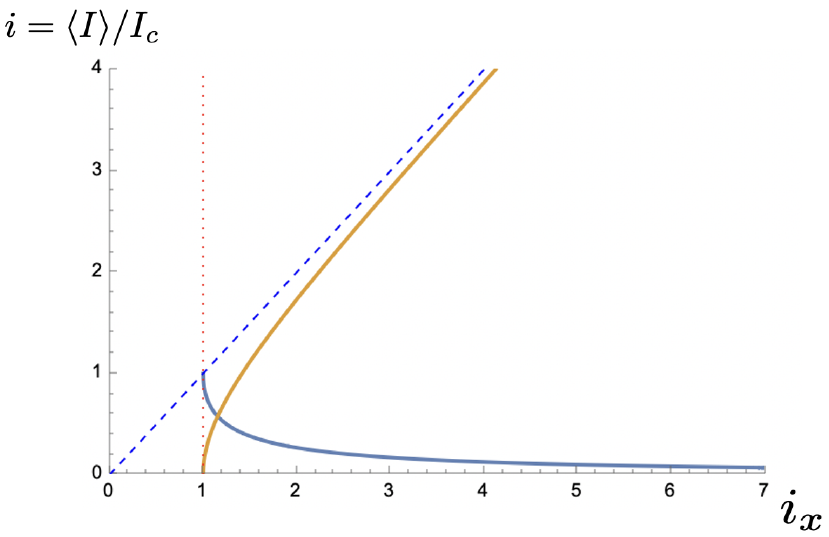
\includegraphics[width=0.5\textwidth]{immagini/current_phase_relation_RCSJ.png}
\end{figure}
\hspace{-0.6cm}Siamo nel regime $i_x>1$. La parte resistiva parte da zero per $i_x=1$ e poi cresce progressivamente. Quanto più aumenta la corrente di bias, tanto più questa relazione tende a diventare lineare.\\
La corrente Josephson, invece, parte da $1$ per $i_x=1$ e poi diminuisce come mostrato nella figura.\\
Riassumiamo quindi i due regimi discussi:
\begin{itemize}[leftmargin=0.5cm]
    \item Per $I_x<I_c$ abbiamo l'\emph{S-state}. In questo caso esistono minimi del potenziale in corrispondenza di
    \begin{equation*}
        \bar{\Phi}=\frac{\Phi_0}{2\pi}\arcsin{\qty(\frac{I_x}{I_c})}
    \end{equation*}
    Questo stato corrisponde a un equilibrio stabile e quindi realizza l'effetto Josephson DC.
    \item Per $I_x>I_c$ abbiamo invece l'\emph{R-state}, poiché compare una componente resistiva. In questo caso non esistono più minimi del potenziale e la particella ``rotola'' lungo il washboard potential. Si manifesta quindi l'effetto Josephson AC, essenzialmente perché $\dot{\varphi} \neq 0$.
\end{itemize}
Questi due regimi, determinati dal valore della corrente di bias, danno quindi luogo rispettivamente all'effetto Josephson DC e all'effetto Josephson AC.\\
Questa è infine la forma tipica della caratteristica corrente--tensione osservata sperimentalmente:
\begin{figure}[H]
    \centering
    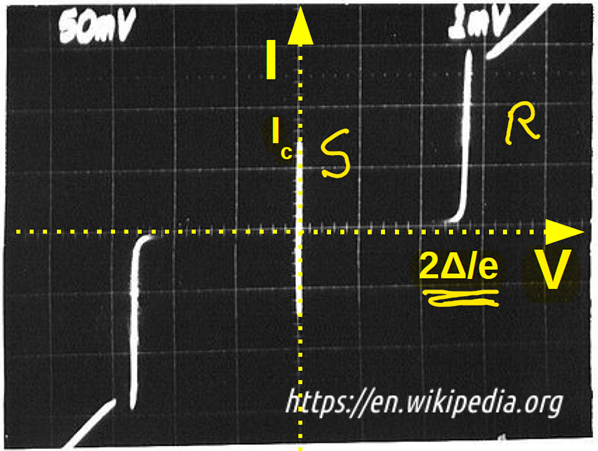
\includegraphics[width=0.5\textwidth]{immagini/IV_characteristic_experiment.png}
\end{figure}
\hspace{-0.6cm}Nel grafico è riportata la corrente in funzione della corrente di bias; equivalentemente possiamo reinterpretarlo come una caratteristica corrente--tensione.\\
Si osserva che:
\begin{itemize}[leftmargin=0.5cm]
    \item a tensione nulla compare lo stato superconduttivo (\emph{S-state});
    \item successivamente compare la parte resistiva.
\end{itemize}
La tensione alla quale compare la parte resistiva corrisponde alla condizione $V>\frac{2\Delta}{e}$, cioè quando l'energia fornita dalla tensione è sufficiente a rompere le coppie di Cooper.
\subsection{Lo stato R: retrapping e isteresi}
Consideriamo ancora la caratteristica corrente--tensione e cerchiamo di capire che cosa accade quando modifichiamo la corrente di bias applicata.
\begin{figure}[H]
    \centering
    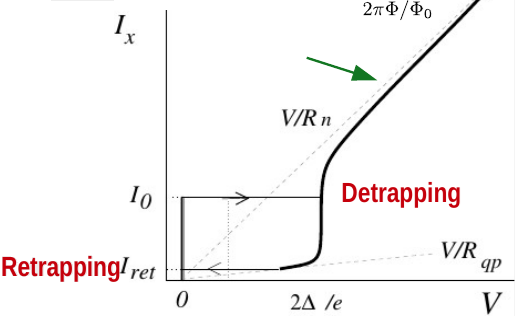
\includegraphics[width=0.6\textwidth]{immagini/IV_characteristic_experiment_2.png}
\end{figure}
\hspace{-0.6cm}Supponiamo di partire da uno stato resistivo, cioè dal regime in cui la particella sta ``rotolando'' lungo il potenziale, e immaginiamo ora di ridurre la corrente di bias, spostandoci a sinistra nel diagramma.\\
Per capire che cosa può accadere, torniamo all'analogia meccanica. Abbiamo una particella che sta scendendo lungo il potenziale e che quindi acquisisce energia cinetica. Ora incliniamo diversamente il potenziale, modificandone la forma in modo tale che compaiano nuovamente dei minimi.\\
Può allora succedere che, se la forma del potenziale viene modificata sufficientemente lentamente, la particella si trovi in un potenziale che possiede dei minimi ma abbia comunque energia cinetica sufficiente per superare le barriere tra un minimo e l'altro.\\
Che cosa significa questo nel grafico? Se partiamo da un certo valore della corrente di bias e poi la riduciamo, modifichiamo progressivamente la forma del washboard potential. Per un certo intervallo il sistema rimane nello stato resistivo, ma a un certo punto può accadere che l'energia acquisita dalla particella durante il moto sia maggiore di quella dissipata.\\
Quando questo accade, la particella può essere nuovamente catturata in uno dei minimi del potenziale e il sistema ritorna nello stato superconduttivo.\\
Se ora percorriamo il processo inverso, cioè partiamo dalla fase superconduttiva e aumentiamo la corrente di bias, può accadere che la particella ritorni nello stato resistivo seguendo però un percorso differente.\\
Si ottiene quindi quello che viene chiamato comportamento isteretico. In particolare:
\begin{itemize}[leftmargin=0.5cm]
    \item quando la corrente di bias viene ridotta si può avere un processo di \emph{retrapping}, nel quale il sistema passa dalla fase resistiva a quella superconduttiva;
    \item viceversa, aumentando la corrente di bias, il sistema può uscire dal minimo del potenziale e tornare nello stato resistivo, in un processo che viene talvolta chiamato \emph{detrapping}.\mn{Si parla di detrapping perché, nello stato resistivo, la particella non è più confinata in un minimo ma scivola lungo il potenziale.}
\end{itemize}
Questo è quindi il comportamento che si osserva in un circuito quando la corrente di bias viene fatta variare avanti e indietro.
\subsection{Comportamento induttivo}
Il passo successivo consiste nell'analizzare il circuito passando gradualmente da regimi in cui la fase si comporta come una variabile classica a regimi in cui essa mostra un comportamento quantistico.\\
Come abbiamo già discusso, in opportune condizioni possiamo quantizzare sia la differenza di fase tra i due lati della giunzione sia la carica presente sugli elettrodi, trattando queste quantità come variabili quantistiche. Questo è possibile perché esse soddisfano una relazione di indeterminazione che deriva originariamente dalla relazione di indeterminazione tra numero e fase del condensato superconduttivo.\\
Il punto importante è che, se la giunzione Josephson è sufficientemente piccola, possiamo entrare in un regime in cui emergono effetti quantistici associati sia alla fase sia alla carica. Si tratta di un comportamento che finora non abbiamo ancora descritto esplicitamente.\\
Per osservare questi effetti è necessario considerare giunzioni di dimensioni sufficientemente ridotte, come avevamo già anticipato. Inoltre vedremo che tali fenomeni compaiono anche in geometrie differenti, incluse configurazioni ad anello nelle quali la fase è direttamente collegata al flusso magnetico.\\
Questa osservazione serve a giustificare il motivo per cui vogliamo ora descrivere il comportamento induttivo della giunzione. Nei circuiti che considereremo comparirà infatti un'induttanza che include anche il contributo della giunzione Josephson stessa, e tale contributo sarà non lineare, come vedremo tra poco. Il passo successivo sarà poi ricavare la forma esplicita delle variabili quantistiche che descrivono l'elemento Josephson all'interno del circuito.\\
Cominciamo considerando una giunzione Josephson nel regime di piccole oscillazioni attorno a un minimo del potenziale.\\
Esprimendo $\varphi$ in termini del flusso magnetico $\Phi$, nel caso di una giunzione inserita in un circuito, il potenziale per un sistema non polarizzato ($I_x=0$) è
\begin{equation*}
    U(\Phi)
    \approx
    -E_J
    \qty[
        1
        -
        \frac{1}{2}
        \qty(
            \frac{2\pi\Phi}{\Phi_0}
        )^2
    ]
    =
    -E_J
    +
    \frac{\Phi^2}{2L_J}
\end{equation*}
dove abbiamo sviluppato il coseno attorno al minimo $\bar{\varphi}=0$.\\
Questa espressione ci permette di identificare immediatamente l'induttanza della giunzione, che è una quantità che avevamo già introdotto in precedenza.\\
Consideriamo ora il caso $0\leq I_x<I_0$. Se sviluppiamo il potenziale attorno a uno dei minimi $\varphi_m\neq0$, corrispondente a un valore del flusso $\bar{\Phi}$, otteniamo
\begin{equation*}
    \begin{split}
        U(\Phi)
        \approx\;
        &U(\bar{\Phi})
        +
        \frac{(\Phi-\bar{\Phi})^2}{2}
        \qty[
            \qty(
                \frac{2\pi}{\Phi_0}
            )^2
            E_J
            \cos{
                \qty(
                    \frac{2\pi\bar{\Phi}}{\Phi_0}
                )
            }
        ]
        \\
        =\;
        &U(\bar{\Phi})
        +
        \frac{(\Phi-\bar{\Phi})^2}{2L_J(I_x)}.
    \end{split}
\end{equation*}
Rispetto al caso precedente compare quindi un termine aggiuntivo nello sviluppo di Taylor, che dipende esplicitamente dalla posizione del minimo.\\
Questo significa che l'induttanza dipende dalla corrente applicata, perché il valore di $\bar{\Phi}$ è legato al minimo $\varphi_m$, e tali minimi dipendono direttamente dalla corrente di bias. In altre parole, se consideriamo il washboard potential e sviluppiamo il potenziale attorno a uno dei suoi minimi, otteniamo un'induttanza differente per ciascun minimo.\\
Questo non è sorprendente, perché stiamo considerando configurazioni fisicamente diverse del sistema, determinate dal valore della corrente di bias che inclina il potenziale.\\
Possiamo quindi descrivere l'elemento Josephson come un elemento la cui induttanza dipende dalla corrente di bias:
\begin{equation*}
    L_J(I_x)
    =
    L_J
    \qty[
        1-
        \qty(
            \frac{I_x}{I_0}
        )^2
    ]^{-1/2}
\end{equation*}
La corrente di bias modifica anche la frequenza di plasma, cosa che risulta naturale perché stiamo considerando oscillazioni attorno a minimi differenti:
\begin{equation*}
    \omega_p(I_x)=\omega_p \qty[ 1- \qty( \frac{I_x}{I_0} )^2]^{1/4}
\end{equation*}
Dobbiamo quindi tenere presente che, variando la corrente di bias, possiamo ottenere differenti valori dell'induttanza Josephson.\\
Questo comportamento non riguarda soltanto configurazioni ad anello, ma vale più in generale per circuiti contenenti giunzioni Josephson, poiché deriva direttamente dalla struttura del washboard potential.
\subsection{Lagrangiana/Hamiltoniana di una giunzione ideale}
Facciamo ora il passo che ci conduce alla quantizzazione del sistema.\\
Consideriamo il modello RCSJ e scriviamo l'equazione in funzione del flusso (che in questo caso rappresenta il flusso del circuito e non necessariamente quello della sola giunzione):
\begin{equation*}
    I_x
    =
    C\ddot{\Phi}
    +
    \frac{\dot{\Phi}}{R}
    +
    I_0
    \sin{
        \qty(
            \frac{2\pi\Phi}{\Phi_0}
        )
    }
\end{equation*}
Se consideriamo il limite underdamped, in cui la resistenza tende all'infinito, possiamo trascurare il termine dissipativo e otteniamo
\begin{equation*}
    I_x
    =
    C\ddot{\Phi}
    +
    I_0
    \sin{
        \qty(
            \frac{2\pi\Phi}{\Phi_0}
        )
    }
\end{equation*}
Vediamo quindi che abbiamo un'equazione equivalente a quella di una particella di massa $C$ che si muove in un potenziale. Possiamo dunque utilizzare gli strumenti della meccanica classica: scrivere una lagrangiana, ricavare da essa l'hamiltoniana e infine quantizzare il sistema imponendo opportune relazioni di commutazione.\\
In questo caso è immediato verificare che l'equazione circuitale senza dissipazione deriva dalla lagrangiana
\begin{equation*}
    \mathcal{L}
    =
    \frac{C}{2}\dot{\Phi}^2
    -
    U(\Phi)
\end{equation*}
dove compare un termine cinetico meno un'energia potenziale, con
\begin{equation*}
    U(\Phi)
    =
    -
    E_J
    \cos{
        \qty(
            \frac{2\pi\Phi}{\Phi_0}
        )
    }
    -
    I_x\Phi.
\end{equation*}
Possiamo ora ricavare il momento coniugato derivando la lagrangiana rispetto alla velocità:
\begin{equation*}
    \pdv{\mathcal{L}}{\dot{\Phi}}
    =
    C\dot{\Phi}
    =
    C(V_L-V_R)
    =
    Q
\end{equation*}
dove abbiamo utilizzato il fatto che $\dot{\Phi}$ può essere espresso in termini della differenza di potenziale ai capi della giunzione. Questa quantità non è altro che la carica della giunzione.\\
Possiamo quindi scrivere l'hamiltoniana:
\begin{equation*}
    \mathcal{H}(Q;\Phi)
    =
    \dot{\Phi}
    \pdv{\mathcal{L}}{\dot{\Phi}}
    -
    \mathcal{L}
    =
    \frac{Q^2}{2C}
    +
    U(\Phi).
\end{equation*}
In particolare, il primo termine rappresenta l'energia elettrostatica. Definendo infatti $q=\frac{Q}{2e}$, esso può essere riscritto come $E_C q^2$.\\
Il motivo per cui introduciamo tutti questi passaggi è che vogliamo costruire un formalismo generale utilizzabile per descrivere circuiti contenenti differenti elementi e differenti geometrie. In circuiti più complessi possono infatti comparire vincoli circuitali e non è immediato identificare le variabili canoniche coniugate.\\
Quello che faremo ora è quindi procedere verso la descrizione quantistica dei circuiti.\\
La manifestazione più tipica del comportamento quantistico di un sistema è la presenza di livelli energetici discreti. La domanda è quindi se sia possibile osservare un comportamento quantistico in un circuito contenente una giunzione Josephson, cioè avere evidenza sperimentale di livelli energetici discreti del circuito. La risposta è naturalmente sì, ma vediamo come.\\
Consideriamo la giunzione nel regime underdamped e nello stato S. Abbiamo già visto che l'energia della giunzione è data dalla somma dell'energia di carica e dell'energia Josephson:
\begin{equation*}
    \mathcal{H}
    =
    \frac{Q^2}{2C}
    -
    E_J
    \cos{
        \qty(
            \frac{2\pi\Phi}{\Phi_0}
        )
    }.
\end{equation*}
Abbiamo inoltre detto che queste variabili possono essere quantizzate.\\
Per capire se il comportamento del sistema sia quantistico oppure no, e in quali condizioni gli effetti quantistici diventino osservabili, possiamo approssimare il potenziale cosinusoidale tramite una successione di pozzi armonici.\\
In questo caso la scala energetica caratteristica è fissata dalla frequenza delle piccole oscillazioni attorno al minimo, cioè
\begin{equation*}
    \hbar\omega_p
    =
    \sqrt{2E_JE_C}
\end{equation*}
Poiché in questo caso non abbiamo corrente di bias, tutti i minimi sono equivalenti e compare semplicemente la frequenza di plasma che abbiamo già introdotto.\\
Se interpretiamo il sistema come una particella classica in un potenziale armonico, abbiamo che:
\begin{itemize}[leftmargin=0.5cm]
    \item la coordinata della particella è la fase;
    \item la quantità analoga all'impulso è la carica;
    \item la massa è sostituita dalla capacità;
    \item la frequenza caratteristica è la frequenza delle piccole oscillazioni attorno al minimo.
\end{itemize}
Otteniamo un comportamento essenzialmente classico quando l'energia di carica è sufficientemente piccola, cioè quando la ``massa efficace'' è grande. In questa situazione la frequenza di plasma è molto minore di $E_J$.\\
Entriamo invece nel regime quantistico quando queste condizioni non sono più soddisfatte e quando la temperatura è sufficientemente bassa rispetto all'energia quantistica delle oscillazioni:
\begin{equation*}
    k_BT
    \ll
    \hbar\omega_p
\end{equation*}
Abbiamo già discusso gli ordini di grandezza tipici dei parametri di una giunzione Josephson. In particolare abbiamo visto che, per giunzioni grandi, osservare effetti quantistici richiederebbe non soltanto temperature estremamente basse, ma anche energie Josephson molto piccole, il che implica barriere molto grandi e quindi giunzioni molto piccole.\\
Per questo motivo, nelle grandi giunzioni Josephson non si osservano effetti di coerenza quantistica, mentre nelle piccole giunzioni tali effetti possono emergere. In questo caso possiamo sperare di osservare la discrezione dei livelli energetici all'interno del potenziale, cioè la presenza di stati quantizzati distinti.\\
Questo effetto è stato osservato sperimentalmente per la prima volta nel 1985. Il circuito utilizzato era una giunzione Josephson in una configurazione che oggi chiameremmo \emph{phase qubit}. In questo caso il potenziale non è semplicemente il coseno periodico, ma assume una forma inclinata con un pozzo metastabile:
\begin{figure}[H]
    \centering
    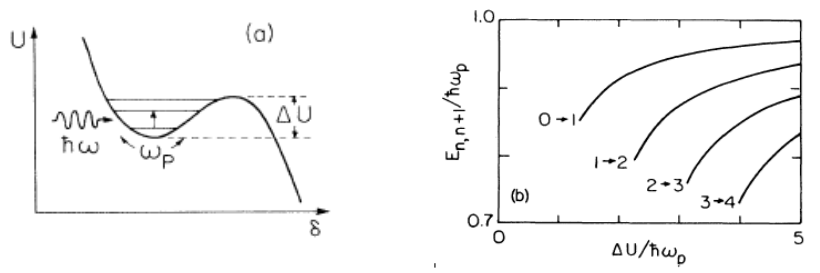
\includegraphics[width=0.9\textwidth]{immagini/potential_phase_qubit.png}
\end{figure}
\hspace{-0.6cm}Se il pozzo di potenziale è sufficientemente profondo, esso può supportare livelli energetici discreti.\\
Vediamo cosa si può fare sperimentalmente. Interpretiamo ancora il problema in termini di particella classica. Se la temperatura è sufficientemente bassa, ad esempio idealmente nulla, la particella rimane nello stato fondamentale.\\
Se ora irradiamo il sistema con una radiazione la cui frequenza è risonante con la prima transizione energetica, può avvenire una transizione verso il primo stato eccitato.\\
Se la particella si trova in uno stato eccitato sufficientemente vicino alla cima della barriera, allora la probabilità di tunneling attraverso la barriera aumenta, perché la barriera effettiva risulta più sottile rispetto a quella vista dallo stato fondamentale.\\
Se questo processo avviene, la coordinata cambia improvvisamente passando dal minimo del potenziale a un valore differente. Di conseguenza compare una derivata temporale della fase diversa da zero:
\[
\dot{\varphi}\neq0.
\]
Ma questo implica immediatamente la comparsa di una tensione ai capi della giunzione. L'evidenza sperimentale del tunneling attraverso la barriera consiste quindi proprio nell'osservazione di una caduta di tensione sulla giunzione.\\
Nel famoso esperimento del 1985 si irradiava il sistema con frequenze differenti, risonanti con differenti transizioni del pozzo di potenziale. Ad esempio, scegliendo una frequenza risonante con la transizione $0\to1$, compariva un picco di corrente associato all'eccitazione del sistema.\\
Ripetendo l'esperimento con frequenze differenti, fu possibile osservare anche le transizioni $1\to2$, eccetera. Inoltre la larghezza della barriera veniva modificata sperimentalmente:
\begin{itemize}[leftmargin=0.5cm]
    \item con una barriera molto piccola era possibile osservare soltanto i primi livelli;
    \item aumentando la barriera diventavano accessibili livelli più elevati, purché la frequenza della radiazione fosse risonante con la corrispondente differenza energetica.
\end{itemize}
Questo esperimento rappresentò la prima osservazione della discrezione dei livelli energetici in un circuito basato su una giunzione Josephson.\\
La descrizione in termini di particella in un potenziale è molto intuitiva, ma bisogna ricordare che il circuito deriva da un sistema superconduttivo. Le transizioni osservate coinvolgono quindi un enorme numero di elettroni, poiché la fase è la differenza di fase tra due condensati superconduttivi.\\
I livelli discreti che osserviamo nel potenziale dipendono dunque da variabili collettive macroscopiche, ed è proprio questa struttura che costituisce la base dell'utilizzo di questi circuiti per realizzare dispositivi quantistici.\\
In pratica, ciò che viene sfruttato è la quantizzazione dei livelli energetici per implementare operazioni che coinvolgono, ad esempio, due livelli del sistema.\\
Con il termine ``operazione'' intendiamo qualcosa di analogo alle operazioni logiche di un computer classico, dove due livelli del circuito giocano il ruolo degli stati $0$ e $1$. La differenza fondamentale è che qui i due livelli sono autostati di un'hamiltoniana quantistica del circuito.\\
I parametri che determinano tale hamiltoniana includono:
\begin{itemize}[leftmargin=0.5cm]
    \item la corrente critica della giunzione;
    \item la capacità della giunzione;
    \item la temperatura;
    \item la corrente di bias applicata;
    \item il campo magnetico, che impone un flusso magnetico.
\end{itemize}
Abbiamo quindi diversi parametri controllabili, sia di natura elettrostatica sia legati direttamente alla realizzazione fisica della giunzione, che possono essere utilizzati per manipolare l'evoluzione dei livelli energetici del circuito quantistico.
\section{Computazione: evoluzione controllata di un sistema fisico (computer)}
Cominciamo a discutere il possibile utilizzo dei sistemi superconduttivi basati sull'effetto Josephson come elementi fondamentali per il calcolo quantistico.
\subsection{Dal bit classico al qubit}
Vediamo innanzitutto l'idea di base che sta dietro al computer quantistico. In un computer classico abbiamo:
\begin{itemize}[leftmargin=0.5cm]
    \item una codifica dell'informazione tramite bit classici;
    \item un'unità di elaborazione (CPU) nella quale l'informazione evolve.
\end{itemize}
L'informazione è quindi codificata in una stringa di $0$ e $1$, che tipicamente corrispondono ai due stati stabili di un circuito classico, e viene poi elaborata tramite l'elettronica del sistema.\\
L'idea del calcolo quantistico consiste invece nel codificare ed elaborare l'informazione utilizzando sistemi quantistici. Questo modifica completamente le regole della computazione.\\
L'idea generale è schematizzata nella figura seguente:
\begin{figure}[H]
    \centering
    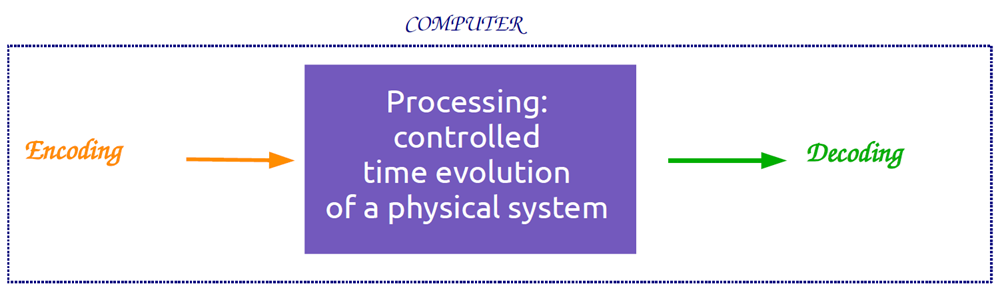
\includegraphics[width=0.8\textwidth]{immagini/computation.png}
\end{figure}
\hspace{-0.6cm}Per un sistema classico l'informazione è codificata in un bit classico (\emph{bit} sta per \emph{binary digit}), che corrisponde tipicamente ai due stati stabili di un circuito classico, ad esempio un circuito elettrico in cui la corrente può fluire oppure no.\\
Se vogliamo interpretare questi due stati come stati di un sistema classico, possiamo immaginarli come i due stati localizzati di una particella in un potenziale a doppio pozzo.
\begin{figure}[H]
    \centering
    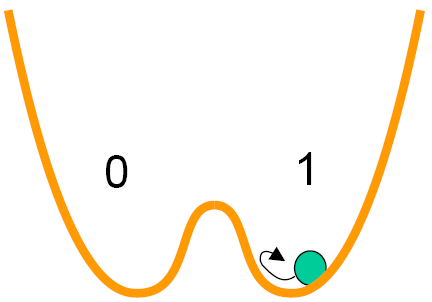
\includegraphics[width=0.4\textwidth]{immagini/double_well_potential_classical.png}
\end{figure}
\hspace{-0.6cm}Supponiamo quindi che i due stati logici derivino dai due stati classici corrispondenti a una particella localizzata in uno dei due minimi del potenziale. Questa è la descrizione tipica di un bit classico.\\
Nel caso quantistico, invece, l'informazione è codificata in un \emph{qubit} (\emph{quantum bit}). L'idea è quindi quella di utilizzare un sistema con due stati quantistici stabili.\\
Se consideriamo ancora il caso del doppio pozzo, sappiamo immediatamente dalla meccanica quantistica quale sia la differenza rispetto al caso classico.
\begin{figure}[H]
    \centering
    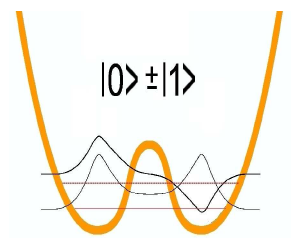
\includegraphics[width=0.35\textwidth]{immagini/double_well_potential_quantum.png}
\end{figure}
\hspace{-0.6cm}Se il sistema è quantistico ed è descritto da un potenziale a doppio pozzo, i due autostati a più bassa energia, indicati con $\ket{0}$ e $\ket{1}$, non corrispondono a stati localizzati nei due minimi, bensì a stati delocalizzati:
\begin{itemize}[leftmargin=0.5cm]
    \item uno con funzione d'onda simmetrica (lo stato fondamentale);
    \item uno con funzione d'onda antisimmetrica.
\end{itemize}
Poiché questi sono stati quantistici, il sistema può trovarsi in una qualsiasi loro combinazione lineare:
\begin{equation*}
    \ket{\psi}
    =
    \alpha \ket{0}
    +
    \beta \ket{1}
\end{equation*}
grazie al principio di sovrapposizione.\\
L'idea dei blocchi fondamentali del calcolo quantistico è quindi analoga a quella del caso classico:
\begin{itemize}[leftmargin=0.5cm]
    \item abbiamo uno stato iniziale in cui l'informazione è codificata, in generale in una sovrapposizione;
    \item abbiamo una \emph{quantum processing unit}, cioè un sistema che evolve quantisticamente. L'evoluzione dello stato segue quindi la dinamica quantistica ed è descritta da un operatore unitario $U(t)$;
    \item l'output della computazione è data dallo stato evoluto:
    \begin{equation*}
        \ket{\psi}_{\rm out}
        =
        \alpha U(t)\ket{0}
        +
        \beta U(t)\ket{1}
    \end{equation*}
\end{itemize}
Sia all'ingresso sia all'uscita abbiamo quindi, in generale, una sovrapposizione di stati.\\
Il fatto che l'evoluzione sia unitaria implica che il dispositivo elabora simultaneamente l'informazione codificata in $\ket{0}$ e in $\ket{1}$. Questo è ciò che prende il nome di \emph{parallelismo quantistico}: la possibilità di operare in parallelo sui due stati di ingresso.\\
Questa è la differenza fondamentale rispetto al caso classico. In un computer classico, infatti, l'ingresso è o $0$ oppure $1$. Se vogliamo elaborare entrambe le informazioni dobbiamo eseguire il processo due volte, una volta preparando il sistema nello stato $0$ e una seconda volta preparando il sistema nello stato $1$.\\
Con un qubit, invece, entrambe le evoluzioni avvengono simultaneamente in un unico processo.\\
Questo vantaggio può sembrare limitato se pensiamo ad un singolo qubit, ma diventa enorme quando consideriamo un gran numero di qubit. Infatti, se abbiamo $N$ qubit, il numero di configurazioni possibili cresce come $2^N$.\\
Il parallelismo quantistico permette quindi di elaborare simultaneamente tutte le informazioni codificate in questo enorme spazio di stati.\\
Tuttavia, questo non è ancora l'aspetto più importante del vantaggio quantistico. Il vero vantaggio del calcolo quantistico emerge soprattutto quando consideriamo sistemi composti da molti qubit ed entra in gioco il concetto di entanglement. L'entanglement consiste nella possibilità di avere stati quantistici di sistemi composti che non sono fattorizzabili nei singoli sottosistemi. In altre parole, possiamo avere stati di più qubit che non possono essere descritti come semplici prodotti degli stati dei singoli qubit.\\
È proprio grazie alla possibilità di creare stati entangled che si possono sviluppare:
\begin{itemize}[leftmargin=0.5cm]
    \item algoritmi quantistici;
    \item protocolli di comunicazione quantistica;
    \item protocolli di crittografia quantistica.
\end{itemize}
Il vantaggio di questi protocolli deriva precisamente dall'entanglement e dalla possibilità di manipolare stati collettivi non fattorizzabili.\\
Le motivazioni profonde e tutte le implicazioni di questi aspetti vanno oltre gli obiettivi del corso.\\
Quello che ci interessa qui è discutere le implementazioni superconduttive dei qubit. La piattaforma superconduttiva presenta infatti numerosi vantaggi pratici e teorici ed è oggi una delle piattaforme più promettenti per la realizzazione di bit quantistici e per l'implementazione del calcolo quantistico.
\subsection{Implementazioni attuali dei qubit}
Diamo ora una panoramica generale delle diverse piattaforme attualmente investigate per l'implementazione dei qubit. Come possiamo vedere, esiste una notevole varietà di approcci.
\begin{figure}[H]
    \centering
    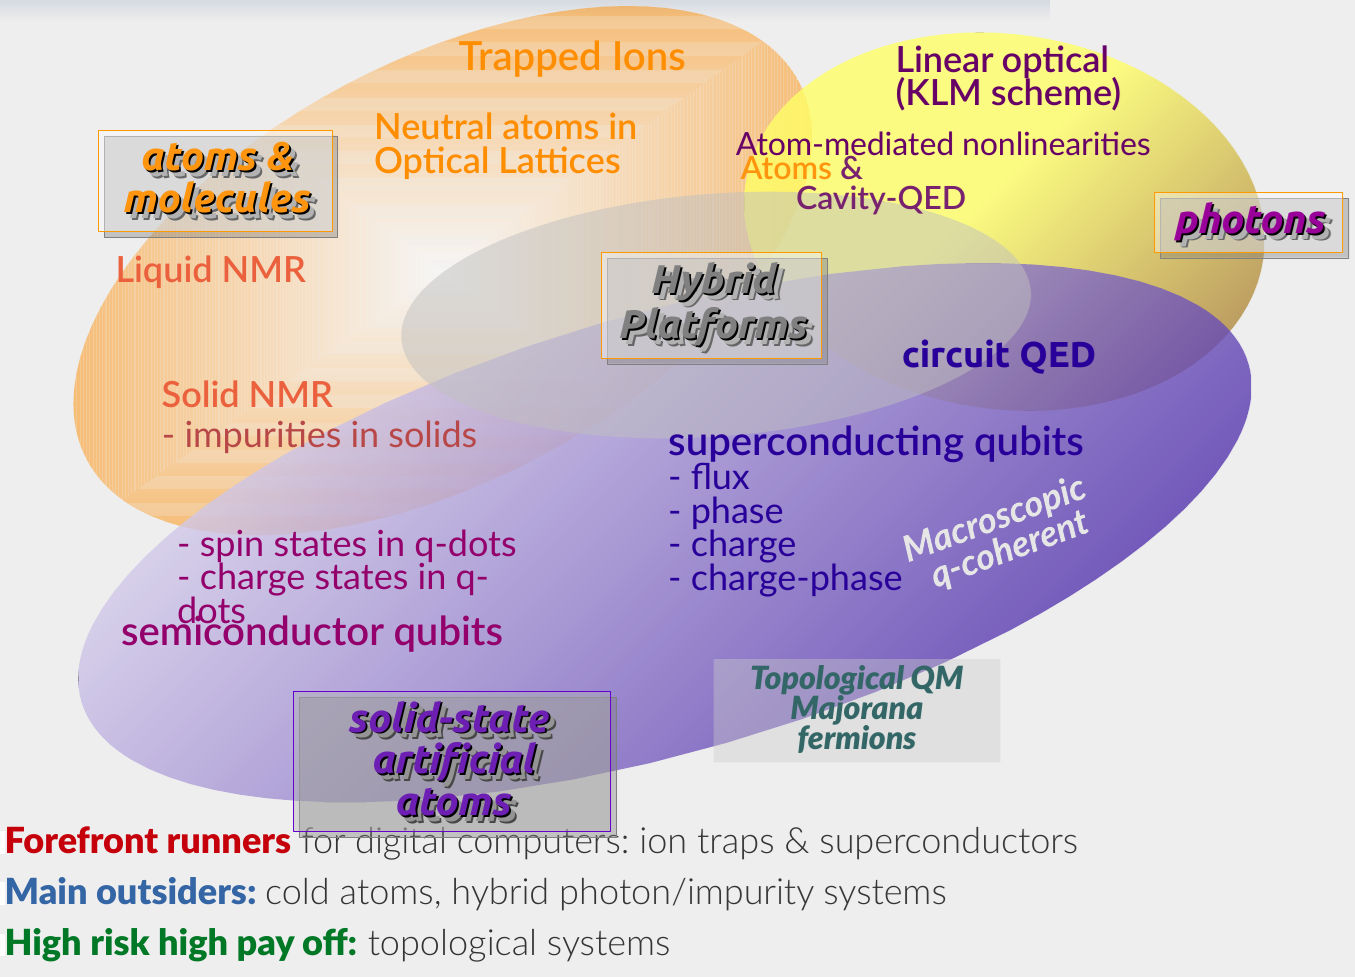
\includegraphics[width=0.8\textwidth]{immagini/quantum_computing_platforms.png}
\end{figure}
\hspace{-0.6cm}I qubit superconduttivi appartengono alla cosiddetta piattaforma \emph{solid state}, e la parola chiave associata a questa piattaforma è \emph{macroscopic quantum coherence}. Abbiamo già utilizzato questi termini per descrivere lo stato BCS di un superconduttore, ed è proprio questo l'ingrediente fondamentale su cui si basano i qubit superconduttivi.\\
Naturalmente non esistono soltanto i qubit superconduttivi. Esistono anche qubit semiconduttivi, che sono essenzialmente di due tipi:
\begin{itemize}[leftmargin=0.5cm]
    \item qubit basati sul grado di libertà di spin;
    \item qubit basati sul grado di libertà di carica.
\end{itemize}
Questi sistemi sono realizzati utilizzando singoli elettroni confinati in \emph{quantum dots} implementati in eterostrutture semiconduttive.\\
L'idea di base è che quanto più piccolo è il quantum dot, tanto più confinato è il potenziale e quindi tanto più discreti e non equidistanti diventano i livelli energetici.\\
L'ingrediente fondamentale è quindi che, in queste eterostrutture artificiali, possiamo creare un potenziale capace di localizzare particelle o elettroni. In tali condizioni possiamo ottenere sistemi a due livelli sufficientemente isolati dagli altri livelli energetici.\\
L'idea generale, indipendentemente dal dispositivo specifico, è quella di avere livelli energetici non equidistanti e utilizzare i due livelli a più bassa energia come qubit.\\
Se il confinamento deriva da un quantum dot, i livelli più bassi possono essere occupati da un elettrone. In questo caso si può:
\begin{itemize}[leftmargin=0.5cm]
    \item utilizzare la carica dell'elettrone (\emph{charge quantum dot});
    \item utilizzare i due stati di spin dell'elettrone come qubit.
\end{itemize}
Oltre a queste piattaforme esistono anche piattaforme più esotiche, ad esempio quelle basate sui fermioni di Majorana.\\
Esistono inoltre piattaforme atomiche e molecolari. Un esempio importante è quello degli atomi neutri intrappolati in reticoli ottici.\\
In questo caso l'idea è utilizzare i sistemi quantistici più semplici possibili, cioè gli atomi, che possiedono naturalmente livelli energetici discreti. Se tali livelli non sono equidistanti, possiamo pensare di utilizzare due livelli atomici come qubit.\\
È chiaro però che, sebbene sia relativamente semplice identificare due livelli atomici, la vera difficoltà consiste nel manipolarli.\\
Infatti, l'obiettivo finale è costruire un oggetto che possa essere utilizzato in maniera analoga ai bit classici:
\begin{itemize}[leftmargin=0.5cm]
    \item dobbiamo manipolare gli stati;
    \item leggere gli stati;
    \item realizzare operazioni logiche;
    \item controllarne l'evoluzione.
\end{itemize}
Fare tutto questo utilizzando singoli atomi è molto più complicato rispetto a una piattaforma a stato solido, dove i livelli quantistici emergono da dispositivi artificiali più facilmente controllabili e manipolabili.\\
Possiamo poi citare anche i fotoni. Anche i fotoni possono essere utilizzati come implementazioni di qubit.\\
A prima vista questo potrebbe sembrare sorprendente, ma bisogna ricordare che i fotoni possiedono un grado di libertà di polarizzazione.\\
Possiamo quindi codificare un sistema a due livelli nella polarizzazione di un singolo fotone propagante lungo un determinato cammino.\\
Un'altra possibilità consiste nel codificare l'informazione nella direzione di propagazione del fotone stesso.\\
I fotoni hanno inoltre il vantaggio di poter essere controllati e manipolati relativamente facilmente, e soprattutto risultano estremamente utili per la comunicazione quantistica grazie alla loro capacità di propagarsi su lunghe distanze, a differenza di oggetti localizzati.\\
Nel seguito ci concentreremo sui dispositivi basati sulla piattaforma superconduttiva.\\
L'elemento fondamentale di questa piattaforma è la giunzione Josephson, perché abbiamo visto che essa:
\begin{itemize}[leftmargin=0.5cm]
    \item è un elemento non lineare;
    \item presenta un comportamento quantistico.
\end{itemize}
Vedremo infatti come questo elemento costituisca il blocco fondamentale per realizzare quelli che vengono spesso chiamati \emph{atomi artificiali macroscopici unidimensionali}.\\
Mostreremo cioè come, utilizzando elementi Josephson, sia possibile fabbricare sistemi a due livelli tunabili, e la possibilità di controllare e modificare i parametri del sistema è un ingrediente cruciale.\\
I due effetti fondamentali che utilizzeremo sono:
\begin{itemize}[leftmargin=0.5cm]
    \item gli effetti di carica. Abbiamo visto che una giunzione Josephson possiede anche un'energia di carica associata al fatto che possiamo isolare un'isola superconduttiva e controllarne la carica. Esiste quindi un costo elettrostatico associato al fatto di caricare oppure no l'isola;
    \item l'effetto Josephson.
\end{itemize}
Vedremo che questi due ingredienti corrispondono a due scale energetiche fondamentali:
\begin{itemize}[leftmargin=0.5cm]
    \item l'energia di carica;
    \item l'energia Josephson.
\end{itemize}
\section{Phase qubit}
Il primo qubit che consideriamo è il cosiddetto phase qubit. Lo introduciamo per primo perché, tra quelli che analizzeremo, è il più semplice alla luce di quanto abbiamo già discusso.\\
Esso consiste essenzialmente in una giunzione Josephson polarizzata in corrente.\\
Abbiamo già ricavato l'hamiltoniana di questo dispositivo. La procedura generale è la seguente:
\begin{itemize}[leftmargin=0.5cm]
    \item si parte dalla descrizione classica del circuito;
    \item si quantizzano carica e fase trattandole come variabili canoniche coniugate;
    \item si costruisce l'hamiltoniana quantistica del circuito.
\end{itemize}
Seguendo questi passaggi otteniamo:
\begin{equation*}
    \hat{\mathcal{H}}
    =
    \frac{\hat{Q}^2}{2C}
    -
    E_J
    \cos{
        \biggl(
            \frac{2\pi\hat{\Phi}}{\Phi_0}
        \biggr)
    }
    -
    I_x\hat{\Phi}
\end{equation*}
che contiene:
\begin{itemize}[leftmargin=0.5cm]
    \item una parte elettrostatica;
    \item una parte Josephson.
\end{itemize}
In questo caso la parte Josephson è espressa in termini del flusso magnetico anziché direttamente della fase, poiché la giunzione è inserita in un circuito ad anello. Inoltre compare un termine aggiuntivo dovuto alla corrente di bias.\\
Abbiamo già visto che il contributo della corrente di bias, sommato all'energia Josephson, genera un potenziale di tipo washboard. Qui ci concentreremo semplicemente su uno dei minimi di questo potenziale.
\begin{figure}[H]
    \centering
    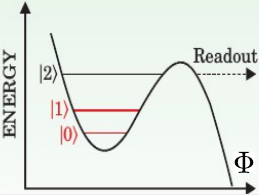
\includegraphics[width=0.5\textwidth]{immagini/washboard_potential_phase_qubit.png}
\end{figure}
\hspace{-0.6cm}L'idea è considerare gli autolivelli energetici all'interno di uno di questi pozzi di potenziale.\\
Se il pozzo è sufficientemente profondo, esso supporta un certo numero di livelli discreti. In particolare ci basta che siano presenti almeno tre livelli:
\begin{itemize}[leftmargin=0.5cm]
    \item i due livelli a energia più bassa, che identificheremo con gli stati $\ket{0}$ e $\ket{1}$;
    \item il terzo livello $\ket{2}$, che vedremo essere importante per il processo di readout.
\end{itemize}
Vediamo ora come emergono questi livelli a partire dall'hamiltoniana del sistema, analizzando in particolare l'energia potenziale.\\
Quello che facciamo è espandere il potenziale attorno a uno dei minimi del washboard potential:
\begin{equation*}
    U(\hat{\Phi})
    \approx
    U(\bar{\Phi})
    +
    \frac{\delta\hat{\Phi}^2}{2L_{Jx}}
    -
    \frac{\lambda_x}{6}
    \delta\hat{\Phi}^3
\end{equation*}
dove abbiamo definito
\[
\delta\hat{\Phi}
=
\hat{\Phi}-\bar{\Phi},
\]
cioè la deviazione del flusso rispetto alla posizione del minimo.\\
Abbiamo inoltre introdotto:
\begin{itemize}[leftmargin=0.5cm]
    \item $L_{Jx}$, cioè l'induttanza efficace della giunzione;
    \item $\lambda_x$, coefficiente associato al termine cubico nello sviluppo del potenziale.
\end{itemize}
Il pedice $x$ serve a ricordare che tale induttanza dipende dalla corrente di bias $I_x$. Infatti nello sviluppo del potenziale compare la derivata seconda valutata nel minimo $\bar{\Phi}$, e la posizione del minimo dipende proprio dalla corrente applicata.\\
Se osserviamo i primi due termini dello sviluppo, riconosciamo immediatamente un oscillatore armonico.\\
Possiamo quindi utilizzare la rappresentazione in seconda quantizzazione dell'oscillatore armonico e riscrivere l'hamiltoniana come
\begin{equation*}
    \hat{\mathcal{H}}
    =
    \hbar\omega_{px}
    \qty(
        \hat{a}^\dagger\hat{a}
        +
        \frac{1}{2}
    )
    -
    \frac{\lambda_x}{6}
    \delta\hat{\Phi}^3
\end{equation*}
dove $\omega_{px}$ è la frequenza delle piccole oscillazioni attorno al minimo.\\
L'idea è quindi trattare il termine non armonico, cioè il termine cubico, come una perturbazione.\\
Applicando la teoria perturbativa otteniamo livelli energetici del tipo
\begin{equation*}
    \varepsilon_n
    =
    \hbar\omega_{px}
    \qty(
        n+\frac{1}{2}
    )
    -
    \frac{\lambda_x}{6}
    \mel*{n}{\delta\hat{\Phi}^3}{n}
    +
    \frac{\lambda_x^2}{36}
    \sum_{m\neq n}
    \frac{ \bigl| \hspace{-0.1cm} \mel*{m}{\delta\hat{\Phi}^3}{n} \hspace{-0.1cm} \bigr|^2}{(n-m)\hbar\omega_{px}}
\end{equation*}
Abbiamo quindi sia il contributo armonico usuale che una correzione perturbativa dovuta all'anarmonicità del potenziale. In particolare stiamo considerando sia il primo sia il secondo ordine della teoria perturbativa.\\
Di conseguenza anche gli autostati vengono modificati:
\begin{equation*}
    \ket{\phi_n}
    =
    \ket{n}
    +
    \lambda_x\ket{\delta_n}
\end{equation*}
Questa è quindi la procedura generale.\\
In pratica il sistema possiede un certo numero di livelli energetici discreti, ma noi ci limiteremo a utilizzare i livelli a energia più bassa per realizzare il qubit.
\subsection{Controllo tramite campi AC}
Vediamo ora come funziona il controllo del phase qubit tramite campi AC.\\
Prima di passare alla derivazione, cerchiamo di capire cosa vogliamo ottenere. Se vogliamo utilizzare il circuito come qubit, naturalmente dobbiamo isolare due livelli, ma poi dobbiamo anche realizzare un certo processing. Fare processing significa manipolare questo stato, cioè fare in modo che il sistema evolva nel modo che desideriamo. Vogliamo farlo intenzionalmente, quindi dobbiamo avere alcuni parametri di controllo che possiamo modificare per far eseguire al sistema le operazioni desiderate. L'unico parametro di controllo che abbiamo in questo caso è la corrente di bias.\\
Possiamo quindi usare la corrente di bias per modificare la forma del potenziale. Possiamo:
\begin{itemize}[leftmargin=0.5cm]
    \item modificarla staticamente, nel qual caso sappiamo che cambia l'inclinazione del potenziale;
    \item modificarla dinamicamente.
\end{itemize}
Poiché la nostra idea è identificare due livelli e poi manipolarli, non vogliamo introdurre variazioni di $I_x$ tali da cambiare completamente il potenziale, ma vogliamo realizzare operazioni tra questi due livelli usando proprio la corrente di bias.\\
L'idea è quindi usare come driving una piccola variazione della corrente di bias dipendente dal tempo. Ad esempio possiamo applicare un drive periodico della corrente, quindi una corrente AC, ma con piccola ampiezza, in modo da non modificare completamente i due livelli, ma soltanto manipolarli in prima approssimazione.\\
Quindi, una volta trovati gli autostati del potenziale, il campo di controllo $\delta I_x(t)$ avrà in generale una certa rappresentazione nella base degli autostati. Per capire come questi autostati evolvono, dobbiamo costruire l'hamiltoniana efficace in un sottospazio che, per ragioni che vedremo più precisamente in seguito, è formato dai primi tre livelli.\\
Se passiamo da una corrente di bias $I_x$ a una corrente $I_x + \delta I_x(t)$, avremo una variazione dell'hamiltoniana data da $-\delta I_x(t)\hat{\Phi}$. La rappresentazione matriciale di tale termine aggiuntivo è
\begin{equation*}
    \hat{\mathcal{H}}_{\rm c}(t)
    =-\delta I_x(t) \hat{\Phi}
    =-\delta I_x(t) \sum_{n,m} \mel*{\phi_m}{\hat{\Phi}}{\phi_n} \ketbra*{\phi_m}{\phi_n}
\end{equation*}
A questo punto vogliamo trovare la rappresentazione matriciale dell'hamiltoniana del phase qubit includendo la corrente di bias.\\
Partiamo dal potenziale originale:
\begin{equation*}
    U(\Phi)
    =- E_J \cos{ \qty( \frac{2 \pi \Phi}{\Phi_0} ) } - I_x \Phi
\end{equation*}
Troviamo i minimi di questo potenziale imponendo $\dv*{U}{\Phi}=0$, da cui otteniamo
\begin{equation*}
    E_J \frac{2 \pi}{\Phi_0} \sin{ \qty( \frac{2 \pi \Phi}{\Phi_0} ) } - I_x
    =0
\end{equation*}
che implica la condizione
\begin{equation*}
    \sin{ \qty( \frac{2 \pi \Phi}{\Phi_0} ) }
    =\frac{I_x}{I_c}
    \qq{dove}
    I_c = \frac{2 \pi E_J}{\Phi_0}
\end{equation*}
Come abbiamo detto, vogliamo espandere il potenziale attorno al minimo in modo da ottenere una parte armonica più una correzione anarmonica. Per fare ciò dobbiamo derivare il potenziale fino al terzo ordine:
\begin{equation*}
    \begin{split}
        \dv[2]{U}{\Phi}
        &=E_J \qty( \frac{2 \pi}{\Phi_0} )^2 \cos{ \qty( \frac{2 \pi \Phi}{\Phi_0} ) }\\[0.2cm]
        \dv[3]{U}{\Phi}
        &= - E_J \qty( \frac{2 \pi}{\Phi_0} )^3 \sin{ \qty( \frac{2 \pi \Phi}{\Phi_0} ) }
    \end{split}
\end{equation*}
Lo sviluppo di Taylor del potenziale attorno al minimo è quindi
\begin{equation*}
    \begin{split}
        U(\Phi)
        & \approx U(\bar{\Phi})
        + \frac{1}{2} E_J \qty( \frac{2 \pi}{\Phi_0} )^2 \cos{ \qty( \frac{2 \pi \bar{\Phi}}{\Phi_0} ) } (\delta\Phi)^2\\[0.2cm]
        & \hphantom{\approx} - \frac{1}{6} E_J \qty( \frac{2 \pi}{\Phi_0} )^3 \sin{ \qty( \frac{2 \pi \bar{\Phi}}{\Phi_0} ) } (\delta\Phi)^3
    \end{split}
\end{equation*}
Ora usiamo la condizione di minimo per scrivere
\begin{equation*}
    \cos{ \qty( \frac{2 \pi \bar{\Phi}}{\Phi_0} ) } 
    =\sqrt{1 - \sin^2{ \qty( \frac{2 \pi \bar{\Phi}}{\Phi_0} ) }}
    =\sqrt{1 - \qty( \frac{I_x}{I_c} )^2 }
\end{equation*}
così da poter riscrivere il potenziale come
\begin{equation*}
    U(\Phi)
    \approx U(\bar{\Phi})
    + \frac{1}{2} E_J \qty( \frac{2 \pi}{\Phi_0} )^2 \sqrt{1 - \qty( \frac{I_x}{I_c} )^2 } (\delta\Phi)^2
    - \frac{1}{6} E_J \qty( \frac{2 \pi}{\Phi_0} )^3 \frac{I_x}{I_c} (\delta\Phi)^3
\end{equation*}
In questo modo abbiamo ottenuto:
\begin{itemize}[leftmargin=0.5cm]
    \item una parte che corrisponde a un potenziale armonico;
    \item una parte che rappresenta una correzione anarmonica al potenziale armonico.
\end{itemize}
Trattiamo ora la parte armonica nel modo usuale, scrivendola in forma quantizzata in seconda quantizzazione. Otteniamo così la seguente hamiltoniana:
\begin{equation*}
    \hat{\mathcal{H}}
    \approx \hbar \omega_{px} \qty( a^\dagger a + \frac{1}{2} ) - \frac{\lambda_x}{6} \delta \hat{\Phi}^3
\end{equation*}
dove $\omega_{px}$ è la frequenza delle piccole oscillazioni attorno al minimo, che dipende dalla corrente di bias, mentre $\lambda_x$ è il coefficiente del termine al terzo ordine nello sviluppo del potenziale attorno al minimo, anch'esso dipendente dalla corrente di bias:
\begin{equation*}
    \lambda_x
    = E_J \qty( \frac{2 \pi}{\Phi_0} )^3 \frac{I_x}{I_c}
\end{equation*}
A questo punto dobbiamo valutare autovalori e autostati. Per gli autovalori, considerando la correzione al primo ordine, dobbiamo calcolare l'elemento di matrice del termine al terzo ordine nello sviluppo del potenziale. Poiché $(\delta \hat{\Phi})^3$ è dispari, si ottiene subito che
\begin{equation*}
    \mel*{n}{(\delta \hat{\Phi})^3}{n}=0
\end{equation*}
A questo punto, l'Hamiltoniana di controllo deve essere valutata sugli autostati corretti\mn{L'idea è che stiamo trattando l'hamiltoniana del potenziale, vista come un potenziale armonico più una correzione anarmonica, come l'hamiltoniana esatta e poi stiamo aggiungendo la perturbazione data dall'hamiltoniana di controllo.}:
\begin{equation*}
    (H_c)_{mn}
    =
    \delta I(t)
    \mel*{\phi_m}{\hat{\Phi}}{\phi_n}
\end{equation*}
Sviluppando al primo ordine in $\lambda_x$, otteniamo
\begin{equation*}
    \mel*{\phi_m}{\hat{\Phi}}{\phi_n}
    \simeq
    \mel*{m}{\hat{\Phi}}{n}
    +
    \mel*{\delta_m}{\hat{\Phi}}{n}
    +
    \mel*{m}{\hat{\Phi}}{\delta_n}
\end{equation*}
Il primo termine fornisce i contributi armonici:
\begin{equation*}
    \Phi_{10}
    \qq{,}
    \Phi_{01}
    \qq{,}
    \Phi_{12}
    \qq{,}
    \Phi_{21}
\end{equation*}
mentre gli altri due termini generano correzioni proporzionali a
$\lambda_x$.
Per esempio, nel limite armonico si ha
\begin{equation*}
    \mel*{0}{\hat{\Phi}}{0}=0,
\end{equation*}
ma utilizzando lo stato corretto
\begin{equation*}
    \ket{\phi_0}
    =
    \ket{0}
    +
    \lambda_x a_0 \ket{1}
    + \cdots
\end{equation*}
otteniamo
\begin{equation*}
    \mel*{\phi_0}{\hat{\Phi}}{\phi_0}
    \simeq
    \lambda_x a_0
    \mel*{0}{\hat{\Phi}}{1}
    +
    \lambda_x a_0^{*}
    \mel*{1}{\hat{\Phi}}{0}.
\end{equation*}
Compare quindi un piccolo contributo diagonale proporzionale a $\lambda_x a_0 \Re(\Phi_{10})$. In maniera analoga, per il primo stato eccitato,
\begin{equation*}
    \ket{\phi_1}
    =
    \ket{1}
    +
    \lambda_x a_1
    \qty(
    \ket{0}+\ket{2}
    )
    + \cdots
\end{equation*}
da cui segue
\begin{equation*}
    \mel*{\phi_1}{\hat{\Phi}}{\phi_1}
    \sim
    \lambda_x a_1
    \Re(\Phi_{01}+\Phi_{21}).
\end{equation*}
Analogamente, per il secondo stato eccitato,
\begin{equation*}
    \ket{\phi_2}
    =
    \ket{2}
    +
    \lambda_x a_2 \ket{1}
    +
    \lambda_x b \ket{3}
    + \cdots
\end{equation*}
si ottiene un termine proporzionale a
\begin{equation*}
    \lambda_x a_2
    \Re(\Phi_{12}+\Phi_{32})
\end{equation*}
Raccogliendo tutti questi contributi, l'Hamiltoniana di controllo $H_c(t)$ nel
sottospazio a tre livelli assume la forma
\begin{equation*}
    \delta I(t)
    \begin{pmatrix}
        a_0 \lambda_x \Re(\Phi_{10})
        &
        \Phi_{01}
        &
        b \lambda_x \Phi_{12}
        \\
        \Phi_{10}
        &
        a_1 \lambda_x \Re(\Phi_{01}+\Phi_{21})
        &
        \Phi_{12}
        \\
        b^{*}\lambda_x (\Phi_{21}+\Phi_{23})
        &
        \Phi_{21}
        &
        a_2 \lambda_x \Re(\Phi_{12}+\Phi_{32})
    \end{pmatrix}
\end{equation*}
Gli elementi di matrice dominanti sono gli accoppiamenti tra livelli
adiacenti $\Phi_{01}, \Phi_{10}, \Phi_{12}, \Phi_{21}$, che sono già presenti nel limite armonico. I termini rimanenti sono invece piccole correzioni generate dall'anarmonicità cubica del
potenziale del phase qubit.\\
Osserviamo ora che i termini proporzionali a $\lambda_x$ rappresentano correzioni piccole dovute all'anarmonicità del potenziale. Nel modello efficace del phase qubit, tali contributi vengono generalmente trascurati al primo ordine, mantenendo solamente gli accoppiamenti dominanti tra livelli adiacenti. Inoltre, l'operatore $\hat{\Phi}$, nel limite quasi armonico, collega principalmente stati con
\begin{equation*}
    \Delta n = \pm 1,
\end{equation*}
mentre gli accoppiamenti diretti tra stati non adiacenti risultano molto più deboli. Aggiungendo quindi il termine di controllo all'Hamiltoniana non perturbata
\begin{equation*}
    \hat{H}_0
    =
    \sum_n \varepsilon_n \ketbra*{n},
\end{equation*}
e trascurando i contributi piccoli proporzionali a $\lambda_x$, otteniamo
l'Hamiltoniana efficace nel sottospazio a tre livelli:
\begin{equation*}
    \hat{H} + \hat{H}_c(t)
    \simeq
    \begin{pmatrix}
        \varepsilon_0
        &
        \delta I_x(t)\Phi_{01}
        &
        0
        \\
        \delta I_x(t)\Phi_{10}
        &
        \varepsilon_1
        &
        \delta I_x(t)\Phi_{12}
        \\
        0
        &
        \delta I_x(t)\Phi_{21}
        &
        \varepsilon_2
    \end{pmatrix}
\end{equation*}
Questa matrice mostra chiaramente che il drive esterno induce principalmente transizioni tra stati adiacenti. In particolare,l'accoppiamento tra $\ket{0}$ e $\ket{1}$ realizza il controllo del qubit,mentre il termine tra $\ket{1}$ e $\ket{2}$ descrive il possibile leakage verso il secondo stato eccitato dovuto alla limitata anarmonicità del
phase qubit. Abbiamo una matrice $3 \times 3$ perché questo dispositivo funziona utilizzando sostanzialmente questi tre stati, i primi due per la computazione e il terzo per il per il readout.\\
Per effettuare il readout del qubit si sfrutta il fatto che il sistema può essere preparato negli stati $\ket{0}$, $\ket{1}$ oppure in una loro sovrapposizione coerente. In tali condizioni l'evoluzione del sistema rimane coerente all'interno del sottospazio dei due livelli.\\
La procedura di misura consiste nell'applicare un impulso risonante con la transizione $\ket{1}\rightarrow\ket{2}$. Se il sistema si trova nello stato $\ket{1}$, l'impulso lo trasferisce nello stato eccitato $\ket{2}$; viceversa, se il sistema si trova nello stato $\ket{0}$, esso rimane sostanzialmente inalterato.\\
Lo stato $\ket{2}$ è scelto in modo da trovarsi molto vicino alla sommità della barriera di potenziale del pozzo considerato. Di conseguenza, una volta popolato tale livello, esiste una probabilità apprezzabile che il sistema attraversi la barriera per effetto tunnel.\\
Dal punto di vista semiclassico, una volta oltrepassata la barriera il sistema si trova in una regione del potenziale in cui quest'ultimo decresce in maniera monotona. La particella equivalente può quindi ``scivolare'' lungo il potenziale, acquisendo una velocità non nulla. In termini della coordinata di fase si ha quindi $\dot{\varphi}\neq 0$. Dalle relazioni di Josephson segue che una variazione temporale della fase corrisponde alla presenza di una differenza di potenziale ai capi della giunzione: $V=\frac{\hbar}{2e} \dot{\varphi}$. Pertanto, se dopo l'applicazione dell'impulso si osserva un impulso di tensione nel circuito, si può concludere che il sistema si trovava inizialmente nello stato $\ket{1}$. In assenza di tale segnale, il sistema era invece nello stato $\ket{0}$.\\
Questo schema realizza quindi una misura dello stato del qubit attraverso il fenomeno del tunneling quantistico macroscopico. Sebbene il sistema venga descritto come una particella efficace che attraversa una barriera di potenziale, tale grado di libertà rappresenta in realtà il condensato superconduttivo nel suo complesso.\\
Finora abbiamo introdotto un termine di driving dipendente dal tempo senza specificarne la forma. Per manipolare il qubit è necessario agire direttamente sulla transizione tra i due livelli logici; a tal fine si applica un drive quasi risonante con la transizione $\ket{0} \to \ket{1}$.\\
In queste condizioni i termini più rilevanti dell'Hamiltoniana appartengono al sottospazio generato dai primi livelli energetici del pozzo. L'effetto principale del drive periodico è quello di indurre transizioni tra gli stati coinvolti, introducendo opportuni elementi fuori diagonale nella rappresentazione matriciale dell'Hamiltoniana.\\
Nel modello considerato manteniamo anche l'accoppiamento con il livello eccitato successivo. Tuttavia, se l'attenzione è limitata al sottospazio bidimensionale che definisce il qubit, l'effetto fondamentale del drive consiste nell'indurre oscillazioni coerenti tra $\ket{0}$ e $\ket{1}$. La forma precisa di tali oscillazioni dipende naturalmente dalla dipendenza temporale del campo applicato.\\
Questo è il meccanismo attraverso cui il sistema viene manipolato. È importante sottolineare che tale risultato è tutt'altro che banale. Stiamo infatti considerando un dispositivo fisico reale, progettato in modo da consentire il controllo dei livelli energetici più bassi di un determinato pozzo di potenziale, analogamente a come nei dispositivi elettronici classici si controllano gli stati logici di un bit.\\
Nei circuiti superconduttivi questo controllo viene ottenuto tramite parametri esterni sperimentalmente accessibili, quali correnti o tensioni applicate. È proprio questa possibilità di indirizzare selettivamente i livelli energetici mediante controlli esterni che rende tali sistemi dei veri e propri ``atomi artificiali''.\\
Un controllo analogo può essere realizzato anche in sistemi atomici naturali. Ad esempio, nella cavity quantum electrodynamics è possibile manipolare con elevata precisione le transizioni atomiche mediante campi elettromagnetici risonanti. Tuttavia, la realizzazione di dispositivi scalabili basati su cavità ottiche presenta notevoli difficoltà tecnologiche.\\
L'obiettivo finale non è infatti controllare un singolo qubit isolato, ma costruire un processore quantistico composto da un gran numero di qubit interagenti. Per questo motivo risultano fondamentali requisiti quali compattezza, controllabilità, integrabilità e scalabilità, del tutto analoghi a quelli che hanno guidato lo sviluppo dell'elettronica moderna.\\
Di conseguenza, ciò che a livello teorico può apparire come un semplice sistema quantistico a pochi livelli rappresenta in realtà la base fisica di una piattaforma concreta per le future tecnologie quantistiche.\\
Quello che possiamo fare è manipolare il sistema. Tuttavia, per realizzare operazioni, non basta soltanto far oscillare coerentemente il sistema avanti e indietro tra i due stati: dobbiamo anche essere in grado di misurarlo, ed è qui che entra in gioco il livello $2$, come avevamo anticipato.\\
Il punto è che questo livello $\ket*{2}$ è vicino alla cima della barriera del potenziale. Possiamo quindi pilotare $I_x$ con lo stesso tipo di accoppiamento, cioè periodico, ma utilizzando frequenze che, invece di essere risonanti con la transizione $0 \to 1$, siano risonanti con la transizione $1 \to 2$. Inoltre, le due transizioni sono fortemente fuori risonanza tra loro, quindi pilotando una non pilotiamo anche l'altra.\\
Se pilotiamo il sistema con la frequenza di transizione $\omega_{12}$, ciò che favoriamo è la transizione tra gli stati $\ket*{1}$ e $\ket*{2}$. Questo significa che, se il sistema si trova nello stato $\ket*{1}$ e applichiamo un drive risonante con la transizione $1 \to 2$, possiamo portare il sistema nello stato $\ket*{2}$.\\
Tuttavia questo stato, essendo vicino alla cima della barriera, ha una probabilità maggiore di attraversare la barriera di potenziale. Se attraversa la barriera, significa che abbiamo una variazione molto rapida nel tempo del flusso magnetico. Ma, tramite la relazione di Josephson, questo è proporzionale alla derivata temporale della tensione.\\
Di conseguenza, ogni volta che avviene una fuga attraverso la barriera compare un impulso di tensione nel circuito. Quello che misuriamo quindi è un impulso di tensione ogni volta che il sistema si trova nello stato $\ket*{1}$. Abbiamo dunque un modo per determinare, tramite un impulso di tensione, se il sistema si trova nello stato $\ket*{1}$, cioè in uno dei due stati computazionali.\\
Se invece il sistema si trova nello stato $\ket*{0}$ e applichiamo un drive con frequenza corrispondente alla transizione $1 \to 2$, non osserveremo alcun impulso di tensione. La distinzione tra gli stati $\ket*{0}$ e $\ket*{1}$ avviene quindi tramite la misura dell'impulso di tensione che compare nella giunzione.\\
Se, ad esempio, il sistema sta oscillando coerentemente tra $\ket*{0}$ e $\ket*{1}$, significa che esiste una certa probabilità di trovarlo nello stato zero oppure nello stato uno, probabilità che oscilla con il coseno della differenza di fase e quindi con la frequenza della transizione. Ciò significa che il sistema oscillerà tra zero e uno con questa frequenza di transizione e, se effettuiamo continuamente la misura mentre pilotiamo anche l'altra transizione, possiamo osservare un comportamento oscillatorio anche nel segnale di misura.\\
Il tipo di misura che stiamo effettuando è quindi un \emph{macroscopic quantum tunneling} stimolato. È:
\begin{itemize}[leftmargin=0.5cm]
    \item \emph{stimolato}, perché è indotto da un drive risonante con la transizione $1 \to 2$;
    \item \emph{macroscopico}, perché ciò che attraversa la barriera tramite tunneling è una quantità macroscopica, dato che $\Phi$ corrisponde alla supercorrente.
\end{itemize}
Vediamo ora cosa si osserva tipicamente:
\begin{figure}[H]
    \centering
    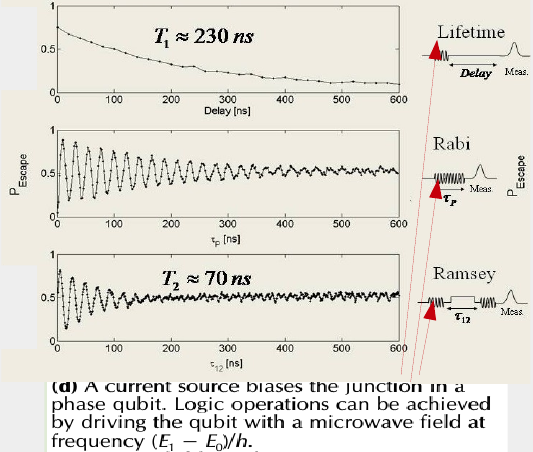
\includegraphics[width=0.5\textwidth]{immagini/phase_qubits_oscillations.png}
\end{figure}
\hspace{-0.6cm}Consideriamo ad esempio le oscillazioni di Rabi, cioè oscillazioni che vengono indotte quando abbiamo un sistema a due livelli pilotato con un drive periodico risonante con la transizione, che è precisamente ciò che facciamo quando applichiamo un drive con frequenza $\omega_{01}$.\\
Quello che osserviamo in queste misure è qualcosa che non ci aspetteremmo. Infatti questo grafico deriva dalla misura degli impulsi di corrente. Misurare questi impulsi equivale in realtà a misurare la probabilità che il sistema si trovi nello stato $\ket*{1}$, che idealmente dovrebbe comportarsi come $\cos^2{(\omega_{01} t)}$. Il punto è che la descrizione basata soltanto sull'hamiltoniana del dispositivo corrisponde a un sistema isolato. In pratica però non abbiamo incluso l'interazione con il resto del circuito. Ad esempio, la cosa più semplice che non abbiamo incluso è la resistenza presente nel circuito.\\
Ma questo non è l'unico effetto: in generale esiste un'interazione del sistema con l'ambiente esterno, che induce un decadimento delle oscillazioni, nel caso più semplice perché abbiamo dissipazione, cioè perdita di energia, quando il sistema è accoppiato all'ambiente.\\
In molti casi questo effetto viene descritto assumendo che la probabilità di trovare il sistema nello stato $\ket*{1}$ abbia la forma
\begin{equation*}
    \mathbb{P}_{\ket*{1}}(t)
    =\cos^2{(\omega_{01} t)} e^{-t/\tau_1}
\end{equation*}
Molto spesso quindi compare un decadimento esponenziale con una scala temporale $\tau_1$, chiamata tempo di rilassamento, che descrive nel caso più semplice le perdite di energia dovute all'interazione con l'ambiente esterno e in particolare con le sorgenti dissipative.\\
Un altro effetto che può comparire è chiamato \emph{leakage}. Il leakage è una proprietà tipica di un sistema multi-livello. In pratica il sistema possiede un certo numero di livelli energetici e noi abbiamo deciso di concentrarci sui due livelli più bassi, il che è ragionevole, ma resta comunque possibile che il sistema esca da questo sottospazio ridotto.\\
Questo decadimento viene generalmente chiamato \emph{decoerenza}, cioè decadimento delle oscillazioni coerenti. In pratica questo rappresenta uno dei principali problemi delle implementazioni a stato solido dei qubit.\\
Quello che abbiamo discusso finora riguarda il phase qubit. In realtà esiste una vera e propria ``giungla'' di qubit basati su giunzioni Josephson:
\begin{figure}[H]
    \centering
    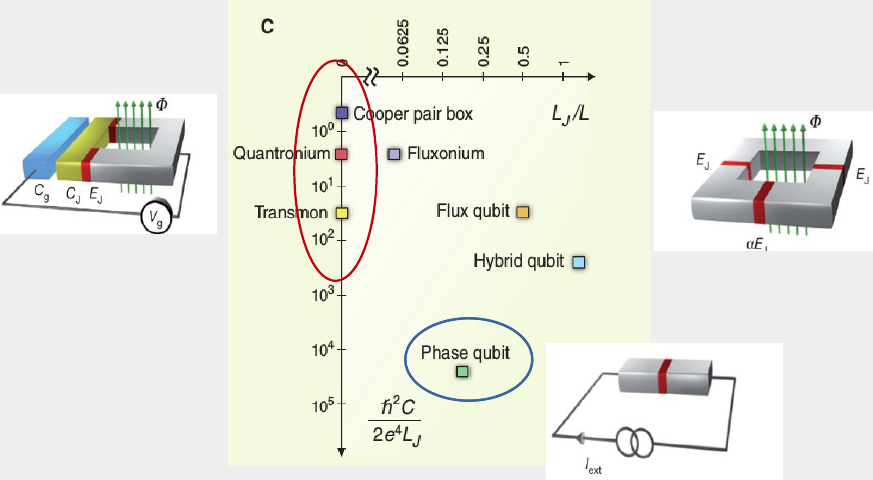
\includegraphics[width=0.8\textwidth]{immagini/jungle_qubits.png}
\end{figure}
\hspace{-0.6cm}La differenza principale tra questi dispositivi è la dimensione delle giunzioni, cioè giunzioni più grandi o più piccole, il che implica avere energie Josephson differenti e anche configurazioni circuitali differenti.\\
Oltre al dispositivo visto finora, esistono infatti architetture molto diverse. Discuteremo ad esempio del Cooper pair box, del Quantronium e del Transmon, che appartengono tutti alla famiglia dei cosiddetti qubit basati sulla carica. L'altra grande famiglia è quella dei qubit basati sul flusso.\\
La distinzione tra queste due famiglie si vede nel diagramma, dove i due parametri sugli assi sono:
\begin{itemize}[leftmargin=0.5cm]
    \item l'induttanza sull'asse $y$;
    \item una combinazione di parametri che scala con la capacità sull'asse $x$.
\end{itemize}
Le configurazioni sono schematizzate nella figura. I qubit basati sul grado di libertà di carica (e vedremo tra poco cosa significa precisamente) hanno una struttura come quella a sinistra, dove la parte gialla è un elettrodo superconduttivo e le due parti rosse sono due giunzioni Josephson. Esse sono collegate a un altro elettrodo, rappresentato in grigio, anch'esso superconduttivo.\\
Il punto importante è che l'elettrodo giallo, che è più piccolo degli altri, si trova di fronte a un altro elettrodo, anch'esso tipicamente superconduttivo. Con questa geometria possiamo considerare la carica accumulata sulla cosiddetta \emph{superconducting island} come una quantità rilevante nel comportamento del dispositivo, e vedremo più avanti in maniera più precisa cosa questo significhi.\\
I qubit basati sulla carica sono quindi dispositivi in cui esiste un elettrodo superconduttivo sul quale possiamo considerare rilevante la carica accumulata. Naturalmente si tratta di carica di coppie di Cooper.\\
L'altra configurazione, chiamata \emph{flux based qubits}, è invece tipicamente basata su un anello superconduttivo interrotto da alcune giunzioni Josephson, generalmente più di una, come si vede nella figura a destra.\\
In questo caso non esiste un'isola speciale: le tre parti del circuito sono più o meno equivalenti e non abbiamo un altro elettrodo posto di fronte all'isola, perché nei dispositivi della famiglia precedente il punto chiave era proprio la presenza di un accoppiamento capacitivo elettrostatico con un elettrodo esterno, cosa che qui non avviene.\\
Di conseguenza, in questo caso il grado di libertà rilevante per codificare l'informazione è l'operatore di flusso.\\
Quindi, a seconda delle dimensioni delle giunzioni e della configurazione circuitale in cui le giunzioni sono inserite, possiamo ottenere dispositivi in cui la variabile quantistica più rilevante è la carica elettrostatica oppure il flusso magnetico.\\
Ricordiamo infine che carica e flusso sono variabili coniugate, quindi le diverse configurazioni circuitali determinano quale delle due variabili diventa dominante nella dinamica del dispositivo.
\section{Cooper pair box}
Descriviamo ora i blocchi fondamentali di questo tipo di circuito. Partiamo dal qubit di carica. Il circuito più semplice è il cosiddetto \emph{Cooper pair box}, cioè una ``scatola'' per coppie di Cooper, schematizzata nel modo seguente:
\begin{figure}[H]
    \centering
    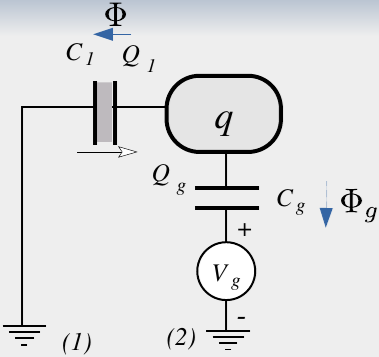
\includegraphics[width=0.45\textwidth]{immagini/Cooper_pair_box.png}
\end{figure}
\hspace{-0.6cm}Abbiamo un'isola superconduttiva, rappresentata come una scatola, che costituisce un elettrodo superconduttivo. Questo elettrodo è isolato dal resto del circuito tramite una giunzione Josephson; quindi ciò che abbiamo schematizzato come la capacità $C_1$ è in realtà una giunzione Josephson.\\
Questa è quindi una descrizione elettrostatica della giunzione e dell'elettrodo, nella quale vogliamo enfatizzare il fatto che la giunzione possiede anche una capacità.\\
Di fronte a questo elettrodo ne abbiamo un altro, con il quale esiste un accoppiamento elettrostatico descritto dalla capacità $C_g$, dove il pedice $g$ sta per ``gate'', perché questo elettrodo è collegato a una sorgente di tensione, la tensione di gate $V_g$.\\
\subsection{L'hamiltoniana}
Quello che dobbiamo fare ora è scrivere la descrizione elettrostatica del circuito considerando la parte elettrostatica e l'energia Josephson. Per la parte elettrostatica dobbiamo semplicemente descrivere il circuito come in elettromagnetismo classico, considerando l'energia elettrostatica associata alla presenza di una certa carica $Q$ sull'isola.\\
Poiché l'isola è accoppiata elettrostaticamente alla tensione di gate, la carica efficace sarà $Q + C_g V_g$, mentre la capacità totale sarà $C_\Sigma$, data dalla somma della capacità della giunzione Josephson e di $C_g$.\\
In aggiunta dobbiamo includere la possibilità di avere energia Josephson. L'hamiltoniana complessiva sarà quindi
\begin{equation*}
    \mathcal{H}=\frac{(Q + C_g V_g)^2}{2 C_{\Sigma}} - E_J \cos{ \qty( \frac{2 \pi \Phi}{\Phi_0} ) }
\end{equation*}
dove abbiamo espresso la differenza di fase in termini del flusso magnetico.\\
Il termine Josephson è quindi il solito termine $- E_J \cos(\varphi)$, e ancora una volta colleghiamo la differenza di fase al flusso magnetico. Anche se qui il circuito non è rappresentato esplicitamente come un anello, bisogna capire che anche in questa configurazione l'energia Josephson può essere espressa in termini del flusso.\\
Questa Hamiltoniana deriva quindi da una descrizione classica del sistema, nel senso che assumiamo che l'elemento Josephson abbia un'energia data da questa espressione.\\
Qual è il passo successivo? Dal momento che siamo partiti scrivendo l'hamiltoniana, dobbiamo verificare che da essa si ottengano correttamente le equazioni del moto delle diverse variabili. A partire dalle equazioni del moto possiamo poi controllare che vengano riprodotte le corrette equazioni circuitali del dispositivo.\\
C'è però un punto importante da considerare. Abbiamo detto che, per una giunzione Josephson isolata, carica e fase sono variabili coniugate. Quando però la giunzione è inserita in un circuito, bisogna identificare correttamente quali siano le variabili coniugate appropriate.\\
Quello che dobbiamo fare è quindi considerare il flusso magnetico come coordinata generalizzata e identificare il momento coniugato. Il punto fondamentale è che il corretto operatore di carica non è necessariamente semplicemente $Q$: bisogna prestare attenzione alla struttura del circuito.\\
In questo caso, diversamente dal phase qubit, la quantità rilevante non è la carica sulla giunzione, ma la carica totale presente sull'isola superconduttiva.\\
Il punto chiave è che la giunzione Josephson e la capacità di gate sono descritte da coordinate generalizzate differenti: $\Phi$ e $\Phi_g$. Dobbiamo quindi prestare molta attenzione alla struttura del circuito.\\
Queste due variabili sono legate dal vincolo imposto dalle cadute di tensione:
\begin{equation*}
    \dot{\Phi} + \dot{\Phi}_g = V_g
\end{equation*}
Il modo corretto di procedere per identificare la variabile coniugata è esattamente lo stesso che si utilizza nella descrizione classica dei sistemi meccanici:
\begin{itemize}[leftmargin=0.5cm]
    \item si parte dalla lagrangiana;
    \item si identificano le variabili coniugate;
    \item si passa all'hamiltoniana;
    \item infine si quantizza il sistema.
\end{itemize}
In altre parole, siamo partiti dall'Hamiltoniana del dispositivo. Quello che dobbiamo fare è verificare che le equazioni di Hamilton riproducano correttamente le equazioni circuitali.\\
Per mostrarlo, procediamo nel verso opposto:
\begin{itemize}[leftmargin=0.5cm]
    \item partiamo dalle equazioni del circuito;
    \item imponiamo i vincoli tra le variabili;
    \item scriviamo il termine cinetico;
    \item identifichiamo la carica tramite le equazioni di Lagrange;
    \item costruiamo l'Hamiltoniana includendo sia il contributo cinetico sia l'energia Josephson.
\end{itemize}
In questo modo ritroveremo l'Hamiltoniana da cui siamo partiti inizialmente.\\
Facciamolo esplicitamente. Partiamo dalla parte cinetica:
\begin{equation*}
    K
    =
    \frac{C}{2} \dot{\Phi}^2 + \frac{C_g}{2} \dot{\Phi}_g^2
    =
    \frac{C}{2} \dot{\Phi}^2 + \frac{C_g}{2} (V_g - \dot{\Phi})^2
\end{equation*}
dove nel secondo passaggio abbiamo utilizzato il vincolo precedente.\\
Ora possiamo identificare la variabile coniugata:
\begin{equation*}
    Q
    =\frac{\partial K}{\partial \dot{\Phi}}
    =C \dot{\Phi} - C_g (V_g - \dot{\Phi})
\end{equation*}
da cui otteniamo
\begin{equation*}
    Q=(C + C_g)\dot{\Phi} -C_g V_g
\end{equation*}
e quindi
\begin{equation*}
    \dot{\Phi}
    =\frac{Q + C_g V_g}{C + C_g}
    =\frac{Q + C_g V_g}{C_{\Sigma}}
\end{equation*}
L'Hamiltoniana sarà data da
\begin{equation*}
    \mathcal{H}
    =Q \dot{\Phi} - K + U(\Phi)
\end{equation*}
Per ottenere la forma finale dell'Hamiltoniana, esplicitiamo il quadrato presente in $K$:
\begin{equation*}
    K
    =\frac{C}{2} \dot{\Phi}^2 + \frac{C_g}{2} (V_g^2 - 2 V_g \dot{\Phi} + \dot{\Phi}^2)
    =\frac{C_{\Sigma}}{2} \dot{\Phi}^2 - C_g V_g \dot{\Phi} + \frac{C_g}{2} V_g^2
\end{equation*}
L'Hamiltoniana è quindi
\begin{equation*}
    \begin{split}
        \mathcal{H}
        & =C_{\Sigma}\dot{\Phi}^2 - C_g V_g \dot{\Phi} - \frac{C_{\Sigma}}{2} \dot{\Phi}^2 + C_g V_g \dot{\Phi} - \frac{C_g}{2} V_g^2 + U(\Phi)
        \\
        & =\frac{C_{\Sigma}}{2} \dot{\Phi}^2 - \frac{C_g}{2} V_g^2 + U(\Phi)
    \end{split}
\end{equation*}
Esprimiamo infine $\dot{\Phi}$ in termini di $Q$:
\begin{equation*}
    \mathcal{H}
    =\frac{(Q + C_g V_g)^2}{2 C_{\Sigma}} - \frac{C_g}{2} V_g^2 + U(\Phi)
\end{equation*}
Il termine $-\frac{C_g}{2} V_g^2$ è una costante che non dipende dalle variabili dinamiche del sistema, quindi possiamo semplicemente assorbirlo in una ridefinizione dell'energia di riferimento. In questo modo otteniamo l'Hamiltoniana finale:
\begin{equation*}
    \mathcal{H}
    =\frac{(Q + C_g V_g)^2}{2 C_{\Sigma}} - E_J \cos{ \qty( \frac{2 \pi \Phi}{\Phi_0} )}
\end{equation*}
\subsection{Quantizzazione e spettro}
In questo modo otteniamo un'Hamiltoniana classica, ma scritta in una forma tale da poter essere immediatamente quantizzata imponendo relazioni di commutazione tra le variabili coniugate. Assumiamo quindi di poter trattare queste quantità come variabili quantistiche e imponiamo la relazione di commutazione canonica. In questo modo otteniamo l'Hamiltoniana quantistica:
\begin{equation}
    \hat{\mathcal{H}}
    =
    E_C \bigl( \hat{q} + q_g \bigr)^2
    -
    E_J \cos{\hat{\phi}}
    \label{eq:hamiltonian_cooper_pair_box}
\end{equation}
dove
\begin{equation*}
    E_C
    =
    \frac{(2e)^2}{2(C + C_g)}
\end{equation*}
è l'energia elettrostatica associata alla presenza di una coppia di Cooper, mentre
\[
q=\frac{Q}{2e}
\qquad\text{e}\qquad
\phi=\frac{2e\Phi}{\hbar}
\]
sono le variabili adimensionali di carica e flusso. Abbiamo inoltre definito
\[
q_g=\frac{C_g V_g}{2e},
\]
che rappresenta la carica di gate adimensionale.\\
Nel procedere con questa quantizzazione dobbiamo tenere presente che, diversamente dal caso di una particella classica descritta da una variabile continua, dove $x$ e $p$ sono variabili coniugate ma $x$ può assumere qualsiasi valore, qui abbiamo quantità discrete. In particolare, la carica è discreta, perché descrive un numero intero addizionale di coppie di Cooper.\\
Dobbiamo tenere conto di questo fatto quando consideriamo le proprietà delle corrispondenti funzioni d'onda. In altre parole, $\hat{q}$ è un operatore che descrive la carica sull'isola, quindi ci aspettiamo che abbia uno spettro discreto, cioè autovalori
\[
q=0,1,2,\ldots
\]
Se $\hat{q}$ ha uno spettro discreto, allora la funzione d'onda deve essere periodica. Questo è esattamente ciò che accade, ad esempio, per una particella classica soggetta a condizioni periodiche al contorno.\\
Lo si vede facilmente osservando che le relazioni di commutazione imposte implicano che $\hat{q}$ sia rappresentato da $-i\partial_\phi$. Questo è naturale, perché la carica è il momento coniugato del flusso, proprio come $p$ è il momento coniugato di $x$, e possiede quindi una rappresentazione analoga.\\
Agendo quindi sulla funzione d'onda corrispondente all'autovalore $q$, abbiamo
\begin{equation*}
    \hat{q} \ket*{q}
    =
    q \ket*{q}
    \implies
    -i \partial_{\phi}\chi_q(\phi)
    =
    q \chi_q(\phi)
\end{equation*}
dove $\chi_q$ è l'autofunzione associata all'autovalore $q$.\\
Questa equazione è semplicemente risolta dalla funzione d'onda
\begin{equation*}
    \chi_q(\phi)
    =
    A e^{iq\phi}.
\end{equation*}
Gli autovalori risultano discreti se e solo se le funzioni d'onda sono periodiche, cioè se
\[
\psi(\phi)=\psi(\phi+2\pi)
\]
Questo fornisce quindi un modo semplice per vedere che la discrezione degli autovalori della carica corrisponde a funzioni d'onda periodiche nella coordinata flusso.\\
Quello che vogliamo ora analizzare è lo spettro, cioè i livelli energetici di questa Hamiltoniana corrispondenti agli autovalori discreti della carica.\\
Per farlo consideriamo l'\eqrefcustom{eq:hamiltonian_cooper_pair_box} e supponiamo inizialmente di non avere il termine Josephson. In queste condizioni l'Hamiltoniana diventa
\begin{equation*}
    \hat{\mathcal{H}}
    =
    E_C \bigl( \hat{q}+q_g \bigr)^2
\end{equation*}
Gli autostati saranno chiaramente autostati dell'operatore carica, perché non compare alcun'altra variabile quantistica. Infatti, in questo caso, l'Hamiltoniana commuta con l'operatore carica:
\[
\bigl[\hat{\mathcal{H}},\hat{q}\bigr]=0,
\]
quindi possiamo trovare autostati comuni:
\begin{equation*}
    \hat{\mathcal{H}}\ket*{\psi_q}
    =
    E_C \bigl(q+q_g\bigr)^2 \ket*{\psi_q}.
\end{equation*}
Gli autolivelli sono quindi
\begin{equation*}
    E_q(q_g)
    =
    E_C \bigl(q+q_g\bigr)^2
    \qq{,}
    q=0,1,2,\ldots
\end{equation*}
Possiamo rappresentare questi autovalori in funzione di $q_g$, quantità che possiamo controllare variando la tensione di gate:
\begin{figure}[H]
    \centering
    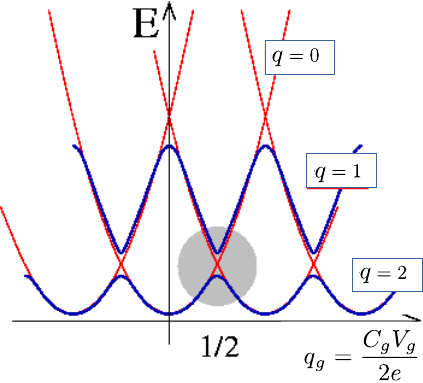
\includegraphics[width=0.5\textwidth]{immagini/parabolas_eigenlevels_CPB.png}
\end{figure}
\hspace{-0.6cm}Ad esempio:
\[
E_0(q_g)=E_C q_g^2,
\]
mentre per $q=1$ abbiamo
\[
E_1(q_g)=E_C(1+q_g)^2,
\]
e così via.\\
Vediamo quindi una serie di parabole, ciascuna associata a un diverso valore di $q$ e con minimo in $q_g=-q$.\\
L'idea è che, fissando nel circuito un determinato valore $\bar{q}_g$, otteniamo un dispositivo fisso i cui autolivelli possono essere letti semplicemente tracciando una linea verticale nel diagramma:
\begin{figure}[H]
    \centering
    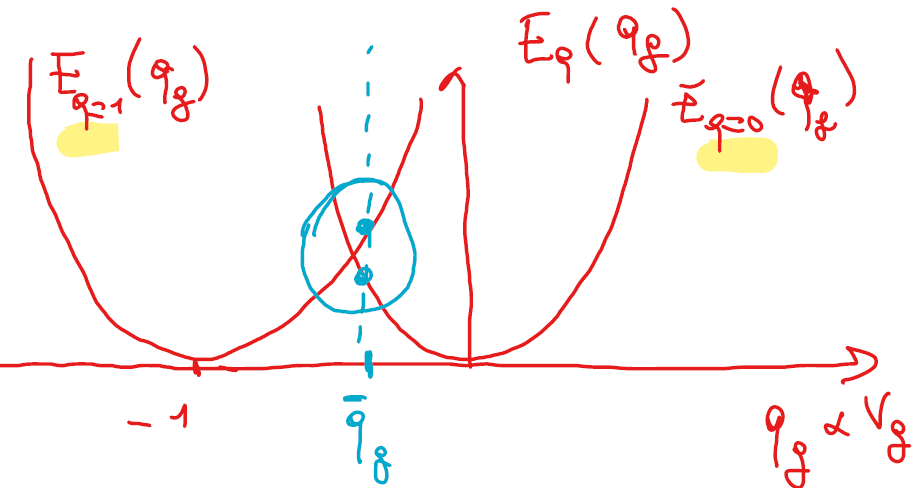
\includegraphics[width=0.5\textwidth]{immagini/parabolas_eigenlevels_CPB_fixed_qg.png}
\end{figure}
\hspace{-0.6cm}Come si vede dalla figura, gli autolivelli superiori sono molto più alti in energia rispetto ai due più bassi. Questo significa che, fissata una tensione di gate, possiamo identificare un sottospazio bidimensionale di autostati completamente isolato energeticamente dagli altri livelli.\\
Questi due livelli energetici più bassi, insieme ai corrispondenti autostati, costituiranno il nostro sottospazio computazionale bidimensionale, cioè gli stati $\ket*{0}$ e $\ket*{1}$ che vogliamo manipolare.\\
Finora abbiamo considerato soltanto la parte elettrostatica, trascurando completamente il termine Josephson. Vogliamo ora capire quale sia l'effetto dell'energia Josephson su questo diagramma.\\
Se operiamo nel cosiddetto \emph{charge regime}, l'energia Josephson è molto più piccola dell'energia di carica. Questo significa che possiamo trattare il termine Josephson come una perturbazione rispetto alla parte elettrostatica.\\
In linea di principio potremmo quindi scrivere le correzioni perturbative agli autolivelli e agli autostati. Tuttavia sappiamo che, dal punto di vista quantistico, la prima cosa che una perturbazione fa in presenza di degenerazioni è rimuoverle.\\
Questo significa che il potenziale viene modificato come mostrato nella figura precedente dalle curve blu, che rappresentano gli autovalori corretti includendo il termine Josephson.\\
Se osserviamo la zona di intersezione tra le parabole, vediamo infatti che la degenerazione scompare: i livelli non si incrociano più, ma vengono separati da un'energia che è proprio dell'ordine dell'energia Josephson.\\
Naturalmente i livelli vengono modificati anche nelle altre regioni, ma lì la correzione è perturbativa. Infatti le curve rosse e blu non coincidono esattamente, ma risultano solo leggermente separate a causa della correzione energetica introdotta dalla perturbazione.\\
Il messaggio principale è quindi che, quando consideriamo sia la parte elettrostatica sia l'energia Josephson, possiamo ancora ottenere — per opportuni valori della tensione di gate, cioè vicino ai punti di quasi-degenerazione — un sistema efficace a due livelli, perché tutti gli altri livelli rimangono molto più alti in energia.\\
Tuttavia, i due livelli non sono più degeneri. Nel caso precedente non ci eravamo posizionati esattamente nel punto di degenerazione, ma leggermente spostati; se ci fossimo messi esattamente nel punto di incrocio avremmo avuto una vera degenerazione.\\
Anche includendo l'energia Josephson, se fissiamo il potenziale vicino a uno di questi punti di quasi-degenerazione, possiamo ancora ottenere un sistema efficace a due livelli sufficientemente isolato dagli altri.\\
Gli autostati, però, non saranno più puri stati di carica: diventeranno sovrapposizioni di stati di carica.
\subsection{Relazioni tra operatori e rappresentazione in carica}
Introduciamo ora la rappresentazione in carica del Cooper Pair Box.\\
Le variabili quantistiche rilevanti sono la differenza di fase superconduttiva $\hat{\phi}$ attraverso la giunzione Josephson e l'operatore $\hat{q}$, che rappresenta il numero di coppie di Cooper presenti sull'isola superconduttiva.\\
Queste due quantità sono variabili canonicamente coniugate e soddisfano la relazione di commutazione
\[
[\hat{q},\hat{\phi}]=i.
\]
Tuttavia, diversamente dal consueto operatore posizione in meccanica quantistica, la fase è una variabile periodica:
\[
\phi \equiv \phi + 2\pi
\]
Per questa ragione, gli operatori fisicamente significativi non sono $\hat{\phi}$ stesso, ma piuttosto funzioni periodiche della fase, come $e^{\pm i\hat{\phi}}$ oppure $\cos\hat{\phi}$.\\
La corretta relazione di commutazione si scrive quindi nella forma
\begin{equation*}
    [\hat{q},e^{\pm i\hat{\phi}}]=\pm e^{\pm i\hat{\phi}}
\end{equation*}
Gli operatori $e^{\pm i\hat{\phi}}$ agiscono come operatori di traslazione nella base di carica. Se $\ket*{q}$ denota uno stato con $q$ coppie di Cooper sull'isola, allora
\begin{equation*}
    e^{\pm i\hat{\phi}} \ket*{q}=\ket*{q \pm 1}
\end{equation*}
L'operatore $e^{+i\hat{\phi}}$ aggiunge quindi una coppia di Cooper all'isola, mentre $e^{-i\hat{\phi}}$ rimuove una coppia di Cooper.\\
Nella base di carica questi operatori possono essere scritti come
\begin{equation*}
    e^{\pm i\hat{\phi}}=\sum_q \ketbra*{q \pm 1}{q}
\end{equation*}
Utilizzando l'identità
\begin{equation*}
    \cos\hat{\phi}
    =
    \frac{1}{2}
    \qty(
        e^{i\hat{\phi}}
        +
        e^{-i\hat{\phi}}
    )
\end{equation*}
otteniamo
\begin{equation*}
    \cos\hat{\phi}
    =
    \frac{1}{2}
    \sum_q
    \ketbra*{q+1}{q}
    +
    \text{h.c.}
\end{equation*}
dove h.c. denota l'hermitiano coniugato.\\
L'Hamiltoniana del Cooper Pair Box può quindi essere scritta nella rappresentazione in carica come
\begin{equation*}
    \hat{\mathcal{H}}
    =
    E_C
    \sum_q
    \bigl(
        q + q_g
    \bigr)^2
    \ketbra*{q}{q}
    -
    \frac{E_J}{2}
    \sum_q
    \bigl(
        \ketbra*{q+1}{q}
        +
        \ketbra*{q}{q+1}
    \bigr).
\end{equation*}
Il primo termine rappresenta l'energia elettrostatica ed è diagonale nella base di carica. Il secondo termine deriva invece dall'accoppiamento Josephson e mescola stati di carica che differiscono di una coppia di Cooper.\\
In altre parole, l'effetto del termine Josephson è quello di indurre transizioni tra gli stati di carica. In particolare, induce transizioni tra gli stati energetici di carica più vicini, che differiscono precisamente per una coppia di Cooper. Per questo motivo, nella rappresentazione in carica esso è un operatore non diagonale: la sua azione consiste nel trasformare lo stato $\ket*{q}$ nello stato $\ket*{q \pm 1}$.\\
Questo è sostanzialmente lo stesso effetto che un operatore quantità di moto produce agendo sugli autostati della posizione. L'operatore quantità di moto, infatti, agisce come generatore di traslazioni. Quindi, se consideriamo autostati della posizione descritti da onde piane e agiamo su di essi con l'operatore quantità di moto, ciò che otteniamo è una traslazione del momento di una certa quantità.
\subsection{Dal Cooper pair box al charge qubit}
Se scegliamo $q_g$ vicino a uno degli stati di energia più bassa, possiamo ridurre lo spazio di Hilbert ai soli stati a energia minima. Matematicamente questo significa proiettare l'Hamiltoniana completa nel sottospazio generato da questi due autostati. Tale proiezione si realizza tramite l'operatore
\begin{equation*}
    \hat{P}
    =
    \ketbra*{0}{0}
    +
    \ketbra*{1}{1}
\end{equation*}
Il risultato è un'Hamiltoniana $2 \times 2$:
\begin{equation*}
    \hat{P}\hat{\mathcal{H}}_{\text{CPB}}\hat{P}
    =
    E_C
    \bigl[
        q_g^2 \ketbra*{0}{0}
        +
        (1+q_g)^2 \ketbra*{1}{1}
    \bigr]
    -
    \frac{E_J}{2}
    \bigl(
        \ketbra*{1}{0}
        +
        \ketbra*{0}{1}
    \bigr).
\end{equation*}
Questa Hamiltoniana consiste di due parti:
\begin{itemize}[leftmargin=0.5cm]
    \item la parte elettrostatica, che possiede due autovalori dipendenti da $q_g$;
    \item la parte Josephson, che agisce nella base di carica come un operatore che scambia gli stati con zero e una coppia di Cooper.
\end{itemize}
Quest'ultimo punto è naturale, perché sappiamo già che l'effetto Josephson corrisponde a una supercorrente che attraversa la giunzione. Se da un lato della giunzione è presente un'isola superconduttiva, allora la supercorrente modifica il numero di coppie di Cooper presenti sull'isola.\\
Poiché stiamo lavorando in un sottospazio $2 \times 2$, possiamo rappresentare l'Hamiltoniana utilizzando le matrici di Pauli.\\
La parte elettrostatica, essendo diagonale nella base di carica, può essere rappresentata tramite $\sigma_z$, mentre la parte Josephson, che è non diagonale nella base di carica, può essere rappresentata tramite $\sigma_x$. In particolare, la parte elettrostatica assume la forma
\begin{equation*}
    E_C
    \begin{pmatrix}
        q_g^2 & 0 \\
        0 & (1+q_g)^2
    \end{pmatrix}
\end{equation*}
Questa matrice può essere riscritta come somma di un termine proporzionale all'identità e di un termine proporzionale a $\sigma_z$:\sn{In generale, una matrice del tipo
\begin{equation*}
    \begin{pmatrix}
        a & 0 \\
        0 & b
    \end{pmatrix}
\end{equation*}
può essere scritta come
\begin{equation*}
    \frac{a+b}{2}\1 + \frac{a-b}{2}\sigma_z
\end{equation*}
dove $\1$ è la matrice identità. Nel nostro caso $a=q_g^2$ e $b=(1+q_g)^2$.}
\begin{equation*}
    E_C
    \begin{pmatrix}
        q_g^2 & 0 \\
        0 & (1+q_g)^2
    \end{pmatrix}
    =
    \frac{E_C}{2}
    \bigl(
        2q_g^2 + 2q_g + 1
    \bigr)\1
    -
    \frac{\epsilon}{2}\sigma_z
\end{equation*}
dove
\begin{equation*}
    \epsilon \equiv \epsilon(q_g)
    =
    E_C(1+2q_g)
\end{equation*}
rappresenta lo splitting energetico tra i due stati di carica.\\
Il termine Josephson in questa rappresentazione è invece dato da
\begin{equation*}
    -\frac{E_J}{2}
    \begin{pmatrix}
        0 & 1 \\
        1 & 0
    \end{pmatrix}
    =
    -\frac{\Delta}{2}\sigma_x
\end{equation*}
dove
\[
\Delta = E_J.
\]
Quindi la proiezione dell'Hamiltoniana del Cooper pair box nel sottospazio degli stati a più bassa energia può essere espressa semplicemente tramite le matrici di Pauli $\sigma_z$ e $\sigma_x$:
\begin{equation*}
    \hat{P}\hat{\mathcal{H}}_{\text{CPB}}\hat{P}
    =
    \frac{E_C}{2}
    \bigl(
        2q_g^2 + 2q_g + 1
    \bigr)\1
    -
    \frac{\epsilon}{2}\sigma_z
    -
    \frac{\Delta}{2}\sigma_x.
\end{equation*}
Spesso il termine proporzionale all'identità viene omesso, perché rappresenta soltanto uno shift energetico globale che non modifica la dinamica del sistema. In tal caso si ottiene l'Hamiltoniana efficace del charge qubit:
\begin{equation*}
    \hat{\mathcal{H}}_{\rm qubit}
    =
    - \frac{\epsilon}{2}\sigma_z
    - \frac{\Delta}{2}\sigma_x
\end{equation*}
dove:
\begin{itemize}[leftmargin=0.5cm]
    \item $\sigma_z$ deriva dalla parte elettrostatica, cioè dall'operatore di carica;
    \item $\sigma_x$ deriva invece dal termine Josephson, cioè dall'operatore di fase.
\end{itemize}
\subsection{Charge qubit pilotato tramite impulsi rapidi}
A questo punto abbiamo fatto qualcosa di molto simile a quanto avevamo fatto per il phase qubit: siamo partiti dalla descrizione circuitale del Cooper pair box, abbiamo identificato autolivelli e autostati e visto che possiamo isolare una coppia di stati a bassa energia che rappresenta il nostro sottospazio computazionale. In definitiva, possiamo trattare il sistema come un sistema efficace a due livelli, cioè il nostro qubit.\\
Il passo successivo consiste nel fare esattamente ciò che abbiamo fatto per il phase qubit: preparare il sistema in un certo stato, lasciarlo evolvere e infine misurarlo. L'evoluzione può essere:
\begin{itemize}[leftmargin=0.5cm]
    \item evoluzione libera, quindi oscillazioni di Maiorana;
    \item oppure un'evoluzione guidata, se vogliamo effettuare operazioni sul qubit, ad esempio oscillazioni di Rabi.
\end{itemize}
In questo caso l'unico parametro di controllo disponibile è la tensione di gate. Possiamo quindi aggiungere alla tensione di gate una componente oscillante nel tempo e ottenere oscillazioni di Rabi nel sistema efficace a due livelli che abbiamo identificato.\\
In generale possiamo considerare una tensione di gate dipendente dal tempo:
\[
q_g \to q_g + \delta q_g(t).
\]
Questo significa aggiungere all'Hamiltoniana una parte di controllo $\hat{\mathcal{H}}_{\text{c}}(t)$, che assume la forma semplice
\begin{equation*}
    \hat{\mathcal{H}}_{\text{c}}(t)
    =
    -E_C \delta q_g(t)\sigma_z
\end{equation*}
poiché $\sigma_z$ è la matrice di Pauli associata all'operatore di carica.\\
L'Hamiltoniana totale di controllo diventa quindi
\begin{equation*}
    \hat{\mathcal{H}}(t)
    =
    -\frac{1}{2}
    \bigl[
        \epsilon + \delta\epsilon(t)
    \bigr]
    \sigma_z
    -
    \frac{E_J(\Phi_x)}{2}\sigma_x
\end{equation*}
dove, invece del solo $\epsilon$, compare
\[
\epsilon + \delta\epsilon(t),
\]
con
\[
\delta\epsilon(t)=2E_C\delta q_g(t),
\]
quantità legata alla tensione di controllo.\\
Con la tensione di gate possiamo fare diverse cose:
\begin{itemize}[leftmargin=0.5cm]
    \item pilotare periodicamente il sistema;
    \item oppure applicare impulsi DC.
\end{itemize}
Nel secondo caso possiamo avere una tensione di gate $V_g(t)$ che non varia periodicamente, ma assume una forma a gradino: ad esempio il gate può essere inizialmente spento, poi acceso per un certo intervallo temporale e infine nuovamente spento.
\begin{figure}[H]
    \centering
    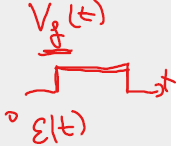
\includegraphics[width=0.3\textwidth]{immagini/pulse_gate_voltage.png}
\end{figure}
\hspace{-0.6cm}Vogliamo fare questo perché modificando la tensione di gate modifichiamo di fatto $\epsilon$, cioè uno dei contributi dell'Hamiltoniana a due livelli, che diventa quindi dipendente dal tempo. In pratica, cambiando $\epsilon$, modifichiamo il peso relativo dei diversi contributi dell'Hamiltoniana.\\
Vediamo questo punto più precisamente. Possiamo rappresentare questa Hamiltoniana tramite la sfera di Bloch, che costituisce una rappresentazione molto conveniente per un sistema a due livelli.\\
In questa rappresentazione abbiamo:
\begin{itemize}[leftmargin=0.5cm]
    \item un asse $z$, associato all'operatore di carica;
    \item un asse $x$, associato all'operatore di fase.
\end{itemize}
Possiamo quindi rappresentare l'Hamiltoniana come un vettore nel piano definito da questi due assi. La componente lungo $z$ è data da $\epsilon$, mentre quella lungo $x$ è data da $\Delta$.\\
Questa rappresentazione è particolarmente utile perché permette di visualizzare immediatamente il peso relativo dei diversi termini dell'Hamiltoniana e l'effetto della variazione dei suoi parametri.\\
Ad esempio:
\begin{itemize}[leftmargin=0.5cm]
    \item se scegliamo una tensione di gate tale da annullare il contributo elettrostatico, l'Hamiltoniana punterà lungo la direzione $x$;
    \item se invece $\epsilon \gg E_J$, l'Hamiltoniana sarà quasi interamente orientata lungo $z$.
\end{itemize}
Possiamo quindi visualizzare l'Hamiltoniana come un vettore sulla sfera di Bloch, la cui direzione dipende dai parametri del circuito.\\
Questa possibilità viene utilizzata per manipolare il charge qubit tramite impulsi rapidi, cioè variazioni improvvise della tensione di gate. Tali impulsi possono essere realizzati con grande accuratezza, su scale temporali dell'ordine delle frazioni di nanosecondo.\\
Vediamo ora come appare l'Hamiltoniana quando modifichiamo la tensione di gate.
\begin{figure}[H]
    \centering
    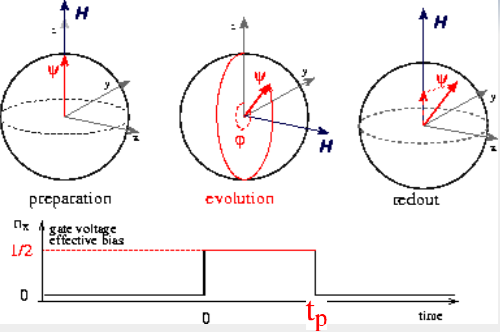
\includegraphics[width=0.6\textwidth]{immagini/bloch_sphere_hamiltonian.png}
\end{figure}
\hspace{-0.6cm}Sull'asse verticale compare $q_x$, legato alla tensione di gate. Partiamo da tensione di gate nulla, con
\[
E_C \gg E_J.
\]
Questo significa che, fintanto che la tensione di gate è nulla, l'Hamiltoniana possiede una componente dominante lungo la direzione $z$. In pratica, il vettore Hamiltoniano punta lungo $z$.\\
Se l'Hamiltoniana punta lungo $z$, i suoi autostati saranno gli autostati di $\sigma_z$. Operando a temperatura sufficientemente bassa, il sistema rilasserà verso lo stato fondamentale dell'Hamiltoniana.\\
Quindi, se manteniamo nulla la tensione di gate e aspettiamo un tempo sufficientemente lungo, il sistema si troverà sicuramente nello stato fondamentale associato alla direzione $z$, rappresentato sulla sfera di Bloch come uno stato allineato con l'Hamiltoniana.\\
Supponiamo ora di accendere molto rapidamente la tensione di gate, portando il sistema al valore
\[
q_x=\frac{1}{2},
\]
che è precisamente il punto in cui i due livelli energetici sono separati soltanto da $E_J$.\\
Matematicamente, per
\[
q_g=\frac{1}{2},
\]
il contributo elettrostatico si annulla e l'Hamiltoniana punta interamente lungo la direzione $\sigma_x$.\\
Poiché questa modifica dell'Hamiltoniana avviene quasi istantaneamente, il sistema non ha il tempo di adattarsi o rilassare verso il nuovo autostato.\\
All'istante iniziale abbiamo quindi:
\begin{itemize}[leftmargin=0.5cm]
    \item un'Hamiltoniana orientata lungo $\sigma_x$;
    \item uno stato iniziale che è invece un autostato di $\sigma_z$.
\end{itemize}
Ma un autostato di $\sigma_z$ è una sovrapposizione degli autostati di $\sigma_x$. Questo significa che il sistema inizierà a oscillare coerentemente tra i due autostati di $\sigma_x$.\\
Sulla sfera di Bloch ciò corrisponde a una precessione attorno alla direzione dell'Hamiltoniana.\\
Questa evoluzione continua fino a quando modifichiamo nuovamente l'Hamiltoniana. Possiamo ad esempio spegnere il gate a un certo istante $t_p$, riportando l'Hamiltoniana nella direzione $z$.\\
In quell'istante il sistema si troverà in una sovrapposizione degli autostati di $\sigma_z$:
\begin{equation*}
    \ket*{\psi(t_p)}
    =
    c_0 \ket*{0}
    +
    c_1 \ket*{1}.
\end{equation*}
Ricordiamo infatti che:
\begin{itemize}[leftmargin=0.5cm]
    \item inizialmente il sistema era preparato in uno stato di $\sigma_z$;
    \item successivamente ha oscillato coerentemente tra gli autostati di $\sigma_x$, cioè $\ket*{+}$ e $\ket*{-}$.
\end{itemize}
L'evoluzione temporale è quindi
\begin{equation*}
    \ket*{\psi(t)}
    =
    \frac{1}{\sqrt{2}}
    \qty(
        e^{iE_J t/2}\ket*{+}
        +
        e^{-iE_J t/2}\ket*{-}
    ).
\end{equation*}
Quando spegniamo l'impulso, otteniamo quindi una sovrapposizione degli stati $\ket*{0}$ e $\ket*{1}$.\\
La probabilità di trovare il sistema nello stato $\ket*{0}$ dipende dalla durata dell'impulso:
\begin{equation*}
    p_0
    =
    |c_0|^2
    =
    \bigl|
        \braket*{0}{\psi(t)}
    \bigr|^2
    =
    \sin^2{
        \qty(
            \frac{E_J t}{2}
        )
    }.
\end{equation*}
Vediamo quindi che la probabilità di trovare il sistema nello stato $\ket*{0}$ dipende:
\begin{itemize}[leftmargin=0.5cm]
    \item dalla durata dell'impulso;
    \item dalla frequenza di oscillazione fissata da $E_J$.
\end{itemize}
Questa è la probabilità di trovare il sistema con zero coppie di Cooper aggiuntive sull'isola. La probabilità di avere invece una coppia di Cooper extra sarà
\[
p_1=1-p_0.
\]
L'ultimo passaggio consiste nel capire come misurare questa probabilità.\\
L'idea è la seguente. Se il sistema possiede una coppia di Cooper aggiuntiva sull'isola, cioè due elettroni extra, esiste una certa probabilità che questa coppia si rompa in quasiparticelle con carica $e$.\\
Questo può avvenire se il circuito è opportunamente collegato a una parte addizionale dedicata alla misura. Quando la coppia di Cooper decade in quasiparticelle, compare una corrente microscopica nel dispositivo di misura.\\
La misura consiste quindi nel rilevare questa corrente associata alla rottura della coppia di Cooper in stati di quasiparticella. Naturalmente questo richiede un ulteriore elemento circuitale dedicato alla lettura dello stato del qubit.
\section{Transmon qubit}
Consideriamo ora il transmon. L'idea è quella di avere un'isola superconduttiva isolata dal resto del circuito tramite la giunzione Josephson e le capacità che la collegano al circuito stesso. Abbiamo già visto che questo dispositivo può avere diverse implementazioni, una delle quali è schematizzata nella figura seguente:
\begin{figure}[H]
    \centering
    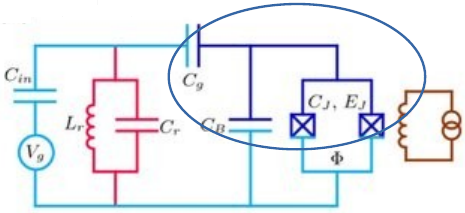
\includegraphics[width=0.6\textwidth]{immagini/transmon.png}
\end{figure}
\hspace{-0.6cm}In questo caso l'isola superconduttiva è la parte blu. Abbiamo quindi un loop superconduttivo interrotto da due giunzioni Josephson e una singola isola superconduttiva collegata al circuito tramite alcune capacità. L'ingrediente aggiuntivo fondamentale è però la capacità $C_B$, posta in parallelo alla giunzione complessiva.\\
Il ruolo di questa capacità addizionale è quello di capacità di shunt. Essa compare infatti nell'energia elettrostatica secondo
\begin{equation*}
    E_C
    =
    \frac{2e^2}{2C_J + C_g + C_S}
\end{equation*}
e, poiché è grande, rende molto più piccola l'energia di carica.\\
In questo modo otteniamo un circuito molto simile al Cooper pair box, ma con un diverso rapporto tra energia di carica ed energia Josephson. Abbiamo già visto che queste due energie giocano un ruolo fondamentale:
\begin{itemize}[leftmargin=0.5cm]
    \item l'energia di carica rende rilevanti gli effetti elettrostatici e quindi la variabile quantistica associata alla carica;
    \item l'energia Josephson rende invece rilevante la variabile quantistica associata alla fase o al flusso.
\end{itemize}
Se il dispositivo opera in questo regime, il primo effetto che osserviamo è una modifica della dipendenza degli autolivelli dalla tensione di gate, come mostrato nella figura seguente:
\begin{figure}[H]
    \centering
    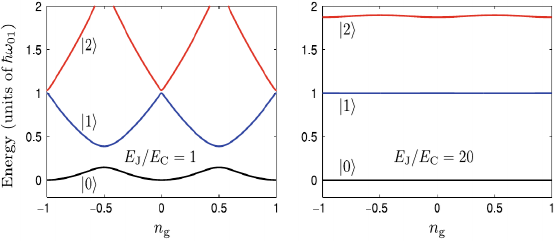
\includegraphics[width=0.7\textwidth]{immagini/transmon_eigenlevels.png}
\end{figure}
\hspace{-0.6cm}Nel grafico di sinistra vediamo gli autolivelli del Cooper pair box quando vengono considerati sia il contributo elettrostatico sia quello Josephson. Abbiamo già commentato che questi livelli dipendono dal parametro di controllo $n_g$, proporzionale alla tensione di gate, e che fissato il valore del gate gli autovalori del dispositivo si ottengono intersecando la verticale corrispondente con i livelli energetici.\\
Ciò che caratterizza il regime di carica, in particolare nel caso in cui $E_J$ ed $E_C$ siano confrontabili, è che i livelli energetici mostrano una forte dipendenza non monotona dalla tensione di gate.\\
Questo implica — e lo vedremo meglio più avanti — che tale implementazione è molto sensibile alle fluttuazioni della tensione di gate provenienti dal circuito elettrostatico. In pratica, anche se vorremmo mantenere il gate fissato a un certo valore, sono sempre presenti fluttuazioni dovute a diverse sorgenti fisiche.\\
Queste fluttuazioni fanno oscillare leggermente il cosiddetto operating point del dispositivo. Di conseguenza, ad esempio, anche lo splitting energetico tra i primi due livelli cambia nel tempo: se il bias fosse perfettamente fissato avremmo uno splitting ben definito, ma se la tensione di gate fluttua allora durante la misura il sistema presenterà valori leggermente diversi dello splitting tra i livelli. Questo costituisce un problema importante, che analizzeremo meglio in seguito.\\
Nel circuito transmon, dove il rapporto tra le due energie è diverso, la dipendenza degli autolivelli dalla tensione di gate diventa molto più debole, come mostrato nella figura di destra.\\
Da un lato questo è vantaggioso perché il sistema risulta meno sensibile alle fluttuazioni della tensione di gate; dall'altro però può creare problemi di addressability, poiché gli splitting energetici diventano sempre più vicini a quelli di un oscillatore armonico. In pratica, ripetendo lo stesso procedimento svolto in precedenza, si vede che gli splitting tra livelli adiacenti diventano molto simili tra loro.\\
Detto questo, poiché vogliamo una grande capacità di shunt per ridurre la sensibilità alle fluttuazioni del gate, cerchiamo di capire come emergano questi splitting energetici.\\
Per farlo procediamo come in precedenza, scrivendo l'Hamiltoniana del dispositivo. In questo caso, poiché l'energia dipende molto debolmente dalla tensione di gate, possiamo considerare un'Hamiltoniana in cui i termini principali sono:
\begin{itemize}[leftmargin=0.5cm]
    \item la parte elettrostatica con la capacità di shunt;
    \item il termine Josephson.
\end{itemize}
Trascuriamo quindi la dipendenza dal gate:
\begin{equation*}
    \hat{\mathcal{H}}
    =
    E_C \hat{Q}^2
    -
    E_J \cos{\hat{\phi}}
    =
    \frac{\hat{Q}^2}{2C+C_S}
    -
    E_J \cos{\hat{\phi}}
\end{equation*}
Per comprendere la struttura degli autovalori, osserviamo che il termine Josephson agisce come un potenziale periodico. Tuttavia, per studiare i livelli a bassa energia non è necessario considerare l'intera periodicità del potenziale: è sufficiente espandere il coseno attorno a uno dei minimi, ad esempio quello in $\phi=0$.\\
Espandendo il coseno otteniamo:
\begin{equation*}
    \hat{\mathcal{H}}
    \approx
    \frac{\hat{Q}^2}{2C+C_S}
    +
    \frac{E_J}{2}\hat{\phi}^2
    -
    \frac{E_J}{4!}\hat{\phi}^4.
\end{equation*}
La forma di questo potenziale è mostrata nella figura seguente:
\begin{figure}[H]
    \centering
    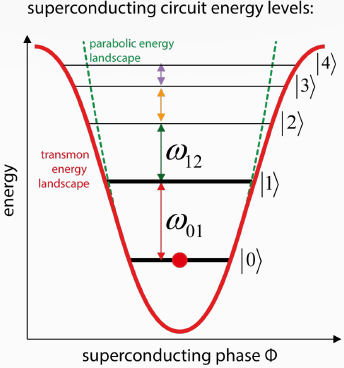
\includegraphics[width=0.4\textwidth]{immagini/transmon_potential.png}
\end{figure}
\hspace{-0.6cm}Vediamo che il potenziale ha forma approssimativamente parabolica vicino al minimo, con una piccola correzione non lineare che diventa importante per valori più grandi di $\phi$.\\
Per piccoli valori di $\phi$, il termine dominante è quindi quello quadratico, mentre il termine quartico introduce l'anarmonicità.\\
Per comprendere gli autovalori del sistema basta allora considerare cosa accadrebbe in un potenziale puramente armonico: avremmo livelli equispaziati. Qui invece, essendo il potenziale leggermente anarmonico, otteniamo livelli leggermente deformati.\\
I primi livelli presentano quindi splitting differenti:
\begin{itemize}[leftmargin=0.5cm]
    \item lo splitting tra i livelli $0$ e $1$ è $\omega_{01}$;
    \item lo splitting tra i livelli $1$ e $2$, cioè $\omega_{12}$, è più piccolo;
    \item e così via.
\end{itemize}
In queste condizioni abbiamo quindi un potenziale anarmonico e possiamo utilizzare il dispositivo come sistema a due livelli concentrandoci sui due livelli più bassi del pozzo di potenziale, che identificano gli stati computazionali $\ket*{0}$ e $\ket*{1}$.
\subsection{Driving e misura}
Abbiamo detto che ci serve un dispositivo con alcuni autolivelli, ma dobbiamo anche essere in grado di effettuare altre due operazioni fondamentali:
\begin{itemize}[leftmargin=0.5cm]
    \item il driving;
    \item la misura.
\end{itemize}
Il driving è simile a quanto fatto per il Cooper pair box: utilizziamo una tensione di gate modulata nel tempo, ad esempio tramite un drive AC periodico. Formalmente, lo descriviamo partendo dall'Hamiltoniana del sistema e aggiungendo un termine di controllo dipendente dal tempo attraverso la modulazione della tensione di gate.\\
La tensione di gate agisce sul grado di libertà di carica e, poiché il nostro obiettivo non è descrivere l'intero sistema multilivello ma solo i livelli a più bassa energia, dobbiamo effettuare una proiezione sul sottospazio bidimensionale generato dagli stati $\ket*{0}$ e $\ket*{1}$.\\
Supponiamo quindi di avere un'Hamiltoniana multilivello della forma
\begin{equation*}
    H
    =
    \sum_n E_n \ketbra*{\psi_n}{\psi_n}.
\end{equation*}
Se vogliamo limitarci ai due livelli più bassi, dobbiamo proiettare l'Hamiltoniana nel sottospazio bidimensionale generato dagli stati $\ket*{0}$ e $\ket*{1}$. Matematicamente introduciamo il proiettore
\begin{equation*}
    P
    =
    \ketbra*{0}{0}
    +
    \ketbra*{1}{1}.
\end{equation*}
La Hamiltoniana proiettata diventa quindi
\begin{equation*}
    PHP
    =
    E_0 \ketbra*{0}{0}
    +
    E_1 \ketbra*{1}{1}.
\end{equation*}
Il risultato può essere espresso anche in termini di matrici di Pauli. Includendo anche il termine di drive otteniamo
\begin{equation*}
    P(H+H_C(t))P
    =
    -\frac{\omega_{10}}{2}\sigma_z
    +
    2E_C \bar{q}_g(t) q_{01}\sigma_x
\end{equation*}
dove
\begin{equation*}
    \sigma_z
    =
    \ketbra*{1}{1}
    -
    \ketbra*{0}{0}
\end{equation*}
e
\begin{equation*}
    \sigma_x
    =
    \ketbra*{0}{1}
    +
    \ketbra*{1}{0}.
\end{equation*}
Il drive deriva dalla modulazione della tensione di gate e quindi entra attraverso l'operatore di carica $\hat{q}$. In questo caso tale operatore è non diagonale, perché gli autostati del sistema non sono più puri stati di carica: l'energia di carica non è infatti la scala energetica dominante.\\
L'idea è quindi che un drive variabile nel tempo, proporzionale a $\sigma_x$, induca transizioni tra gli stati $\ket*{0}$ e $\ket*{1}$. Questo fornisce un modo per manipolare il sistema ed effettuare operazioni sul qubit.\\
Dobbiamo ora affrontare il problema della misura.\\
Nel Cooper pair box avevamo visto una misura di tipo \emph{quantum demolition}: quando il sistema si trovava nello stato con una coppia di Cooper extra, si lasciava decadere quella coppia in quasiparticelle. In altre parole, la misura distruggeva lo stato quantistico originario.\\
Uno dei vantaggi del transmon non riguarda solo il diverso rapporto tra energia di carica ed energia Josephson, ma anche il fatto che la misura può essere effettuata in modo \emph{quantum non demolition} (QND).\\
Vediamo cosa significa. Supponiamo di avere un qubit con Hamiltoniana
\begin{equation*}
    H
    =
    \frac{\omega_{10}}{2}\sigma_z
    =
    \frac{\omega_{10}}{2}
    \qty(
        \ketbra*{1}{1}
        -
        \ketbra*{0}{0}
    ).
\end{equation*}
Effettuare una misura significa verificare, dopo l'evoluzione del sistema, se esso si trovi nello stato $\ket*{0}$ oppure nello stato $\ket*{1}$.\\
Una misura demolitrice implica che, se il sistema è inizialmente in una sovrapposizione
\begin{equation*}
    \ket*{\psi}
    =
    a\ket*{0}
    +
    b\ket*{1},
\end{equation*}
e misuriamo ad esempio lo stato $\ket*{1}$, allora dopo la misura il sistema collassa definitivamente in $\ket*{1}$: la sovrapposizione viene distrutta.\\
Una misura non demolitrice invece mira a ottenere informazione sul sistema senza distruggere la sovrapposizione.\\
Questo può essere fatto accoppiando il qubit a un dispositivo di misura. Supponiamo, ad esempio, che il dispositivo di misura sia un altro sistema a due livelli descritto da $\tau_z$. In questo caso dobbiamo considerare:
\begin{itemize}[leftmargin=0.5cm]
    \item l'Hamiltoniana del qubit;
    \item l'Hamiltoniana del dispositivo di misura;
    \item il termine di accoppiamento.
\end{itemize}
Otteniamo quindi
\begin{equation*}
    H
    =
    \frac{\omega_{10}}{2}\sigma_z
    +
    \frac{\Delta}{2}\sigma_z\tau_z
    +
    \frac{\omega_m}{2}\tau_z
\end{equation*}
dove:
\begin{itemize}[leftmargin=0.5cm]
    \item il primo termine descrive il qubit;
    \item il terzo termine descrive il meter;
    \item il secondo termine rappresenta l'accoppiamento tra i due sistemi.
\end{itemize}
L'accoppiamento è del tipo $\sigma_z\tau_z$, cioè coinvolge gli stessi operatori che compaiono nelle Hamiltoniane dei due sistemi.\mn{Questo significa che il meter ``legge'' lo stato energetico del qubit senza indurre transizioni tra $\ket*{0}$ e $\ket*{1}$, perché il termine di accoppiamento commuta con l'Hamiltoniana del qubit.}\\
Possiamo riscrivere l'Hamiltoniana nella forma
\begin{equation*}
    H
    =
    \frac{\omega_{10}}{2}\sigma_z
    +
    \frac{1}{2}
    \qty(
        \Delta\sigma_z
        +
        \omega_m
    )\tau_z.
\end{equation*}
Quello che vogliamo misurare è il meter.\\
Se il meter fosse isolato, lo splitting dei suoi livelli sarebbe semplicemente $\omega_m$. Quando però esso è accoppiato al qubit, il suo splitting diventa
\[
\omega_m \pm \Delta,
\]
a seconda dello stato del qubit:
\begin{itemize}[leftmargin=0.5cm]
    \item $\omega_m+\Delta$ se il qubit è in $\ket*{1}$;
    \item $\omega_m-\Delta$ se il qubit è in $\ket*{0}$.
\end{itemize}
Misurando quindi la frequenza del meter possiamo determinare lo stato del qubit.\\
Il punto fondamentale è che questa misura non altera lo stato del qubit, proprio perché l'accoppiamento avviene tramite $\sigma_z$, che commuta con l'Hamiltoniana del qubit. Per questo motivo la misura è di tipo quantum non demolition.\\
Vediamo ora come si realizza fisicamente questo tipo di accoppiamento:
\begin{figure}[H]
    \centering
    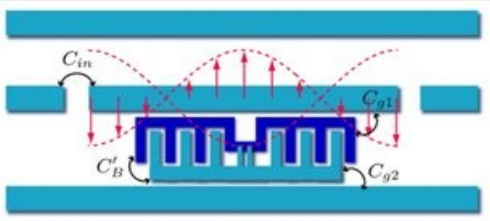
\includegraphics[width=0.5\textwidth]{immagini/Transmon_coupling.png}
\end{figure}
\hspace{-0.6cm}Osserviamo anzitutto la parte inferiore della figura. Abbiamo una regione superconduttiva blu scura, la giunzione Josephson e un secondo elettrodo azzurro chiaro. Questi due elettrodi formano la giunzione Josephson.\\
La giunzione è accoppiata a un microstrip resonator, cioè una linea conduttrice che funziona come risonatore elettromagnetico unidimensionale.\\
Poiché si tratta di un conduttore di lunghezza fissata, esso possiede modi risonanti elettromagnetici e può essere descritto circuitalmente come un circuito LC.\\
Questo risonatore è accoppiato capacitivamente al transmon tramite la capacità $C_g$.\\
Si può dimostrare che, in opportune condizioni, l'accoppiamento tra il dispositivo e il risonatore assume proprio la forma discussa in precedenza. Inoltre, anche in questo caso possiamo limitarci ai due livelli più rilevanti del sistema.\\
La figura seguente mostra il principio della misura:
\begin{figure}[H]
    \centering
    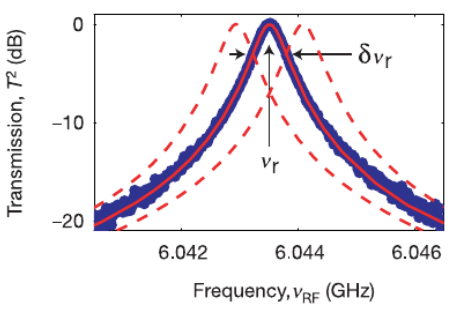
\includegraphics[width=0.7\textwidth]{immagini/Transmon_coupling_measurement.png}
\end{figure}
\hspace{-0.6cm}Quello che viene misurato è la trasmissione della linea risonante, cioè la capacità del risonatore di trasmettere segnali a una certa frequenza.\\
Se il risonatore fosse isolato, la trasmissione massima si avrebbe alla frequenza di risonanza $\omega_m$, rappresentata dalla linea continua.\\
Quando però il risonatore è accoppiato al qubit, la frequenza di risonanza si sposta di una quantità che dipende dallo stato del qubit. Le due linee tratteggiate rappresentano infatti le due possibili frequenze di risonanza del risonatore:
\begin{itemize}[leftmargin=0.5cm]
    \item una corrispondente al qubit nello stato $\ket*{0}$;
    \item l'altra corrispondente al qubit nello stato $\ket*{1}$.
\end{itemize}
Misurando quindi la trasmissione del risonatore in funzione della frequenza possiamo determinare lo stato del qubit a cui esso è accoppiato.\\
Questa misura è di tipo non demolition rispetto al qubit proprio grazie alla particolare forma dell'accoppiamento, che permette di leggere il risonatore senza alterare direttamente lo stato del qubit.
\section{Flux qubit}
Studiamo ora il flux qubit. La famiglia dei flux qubit è caratterizzata da una geometria ad anello nella quale sono presenti una o più giunzioni Josephson. In questo caso non abbiamo un elettrodo posto di fronte a una delle parti dell'anello, quindi il contributo dovuto all'energia di carica è assente oppure fortemente ridotto.\\
Il principale parametro esterno utilizzato per controllare il sistema è un campo magnetico che produce un flusso attraverso l'anello, fenomeno che sappiamo essere associato a proprietà come la quantizzazione del flusso.\\
Abbiamo già studiato l'RF-SQUID. Si tratta di uno SQUID interrotto da giunzioni Josephson e abbiamo visto che può essere utilizzato per effettuare misure estremamente sensibili di campi magnetici.\\
Se vogliamo descrivere il circuito equivalente, la struttura è molto semplice:
\begin{itemize}[leftmargin=0.5cm]
    \item abbiamo l'elemento Josephson;
    \item una geometria ad anello;
    \item un effetto capacitivo dovuto alla giunzione;
    \item e un contributo induttivo associato al loop.
\end{itemize}
Abbiamo già scritto l'equazione circuitale ottenuta dalla descrizione elettrostatica del dispositivo tramite le relazioni Josephson:
\begin{equation*}
    C \ddot{\Phi}
    +
    I_c \sin{
        \qty(
            \frac{2\pi\Phi}{\Phi_0}
        )
    }
    +
    \frac{\Phi+\Phi_x}{L}
    =
    0
\end{equation*}
dove:
\begin{itemize}[leftmargin=0.5cm]
    \item il secondo termine deriva dall'effetto Josephson;
    \item il terzo termine deriva invece dal flusso magnetico e dall'induttanza del loop.
\end{itemize}
Questi ultimi due termini definiscono il potenziale del sistema, ottenuto integrando rispetto al flusso:
\begin{equation*}
    U(\Phi)
    =
    -E_J \cos{
        \qty(
            \frac{2\pi\Phi}{\Phi_0}
        )
    }
    +
    \frac{(\Phi+\Phi_x)^2}{2L}.
\end{equation*}
Esso consiste quindi nella somma:
\begin{itemize}[leftmargin=0.5cm]
    \item dell'energia Josephson;
    \item dell'energia induttiva.
\end{itemize}
Questo potenziale svolge il ruolo di un potenziale efficace. La sua forma è relativamente semplice da comprendere:
\begin{itemize}[leftmargin=0.5cm]
    \item abbiamo un contributo parabolico in $\Phi$, con minimo in $\Phi=-\Phi_x$;
    \item a questo si sovrappone il termine coseno, che introduce una periodicità.
\end{itemize}
Il risultato è quindi un potenziale parabolico modulato periodicamente.
\begin{figure}[H]
    \centering
    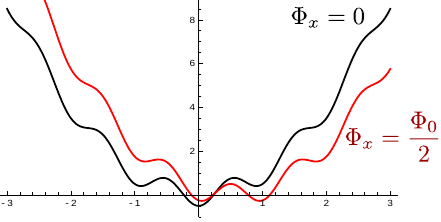
\includegraphics[width=0.6\textwidth]{immagini/flux_qubit_potential.png}
\end{figure}
\hspace{-0.6cm}La forma del potenziale dipende dal valore di $\Phi_x$, cioè dal flusso del campo magnetico esterno.\\
Ricordiamo infatti che, in una geometria ad anello, il flusso totale dipende sia dal campo magnetico applicato esternamente sia dal campo magnetico generato dalla supercorrente che circola nel loop.\\
A seconda del valore di questo flusso, il potenziale può assumere forme differenti e possedere minimi in posizioni diverse.\\
Ad esempio, se
\[
\Phi_x=0,
\]
la struttura del potenziale presenta un unico minimo in $\Phi=0$.\\
Il contributo armonico ha minimo nullo in quel punto, mentre il termine coseno fornisce il contributo $-E_J$, motivo per cui il minimo dell'energia risulta minore di zero.\\
Alla parte armonica molto dolce si sovrappone quindi il termine oscillatorio del coseno. Tuttavia, poiché il termine parabolico cresce per valori grandi di $\Phi$, l'effetto relativo delle oscillazioni del coseno diventa progressivamente meno rilevante e il potenziale appare via via più regolare.\\
Se invece
\[
\Phi_x\neq 0,
\]
i minimi del potenziale si modificano. In particolare, quando
\[
\Phi_x \approx \frac{\Phi_0}{2},
\]
il potenziale assume una forma a doppio pozzo, con due minimi distinti.\\
La forma del potenziale è all'origine della natura degli stati a più bassa energia del sistema. Prima di analizzarli, vediamo come descrivere formalmente il circuito.\\
Dobbiamo:
\begin{itemize}[leftmargin=0.5cm]
    \item scrivere l'equazione circuitale;
    \item identificare il potenziale;
    \item costruire la lagrangiana usando come variabili $\Phi$ e $\dot{\Phi}$.
\end{itemize}
La lagrangiana è
\begin{equation*}
    \mathcal{L}(\Phi,\dot{\Phi})
    =
    \frac{C}{2}\dot{\Phi}^2
    +
    E_J \cos{
        \qty(
            \frac{2\pi\Phi}{\Phi_0}
        )
    }
    -
    \frac{(\Phi+\Phi_x)^2}{2L}.
\end{equation*}
Dalla lagrangiana possiamo identificare il momento coniugato:
\begin{equation*}
    \pdv{\mathcal{L}}{\dot{\Phi}}
    =
    C\dot{\Phi}
    \equiv
    Q.
\end{equation*}
Una volta note le due variabili coniugate, possiamo scrivere l'Hamiltoniana, costituita dalla parte cinetica e da quella potenziale, e quantizzarla imponendo le relazioni di commutazione canoniche:
\begin{equation*}
    \hat{\mathcal{H}}
    =
    \frac{\hat{Q}^2}{2C}
    +
    \frac{(\hat{\Phi}+\Phi_x)^2}{2L}
    -
    E_J
    \cos{
        \biggl(
            \frac{2\pi\hat{\Phi}}{\Phi_0}
        \biggr)
    }
    \qq{,}
    \bigl[
        \hat{\Phi},
        \hat{Q}
    \bigr]
    =
    i\hbar.
\end{equation*}
Questo procedimento è esattamente analogo a quello seguito per gli altri circuiti.\\
Bisogna però ricordare una differenza fondamentale rispetto al charge qubit. Nel charge qubit la carica sulla giunzione è discreta, perché l'isola può contenere un numero intero di coppie di Cooper:
\[
0,1,2,\ldots
\]
Nel flux qubit, invece, non abbiamo un'isola isolata. Di conseguenza la carica non è discreta ma continua.\\
Questo è collegato anche al fatto che il potenziale non è periodico nella coordinata $\Phi$. Possiamo quindi imporre le usuali condizioni al contorno standard, senza necessità di imporre condizioni periodiche come nel caso del Cooper pair box.\\
Vediamo ora come viene generato il campo magnetico esterno.
\begin{figure}[H]
    \centering
    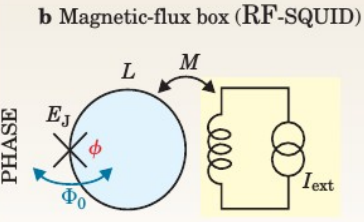
\includegraphics[width=0.5\textwidth]{immagini/flux_qubit_external_field.png}
\end{figure}
\hspace{-0.6cm}È sufficiente avere un altro circuito nelle vicinanze, percorso da corrente. Questo circuito è accoppiato induttivamente all'anello superconduttivo e produce quindi un accoppiamento magnetico tra i due sistemi.\\
Consideriamo ora l'ingrandimento del paesaggio di potenziale nel caso
\[
\Phi_x=\Phi_0.
\]
\begin{figure}[H]
    \centering
    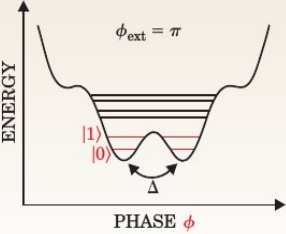
\includegraphics[width=0.5\textwidth]{immagini/flux_qubit_double_well.png}
\end{figure}
\hspace{-0.6cm}Questa figura rappresenta un ingrandimento della configurazione corrispondente alla curva rossa del grafico precedente, nella quale osserviamo chiaramente la presenza di due minimi del potenziale.\\
Qui iniziamo a passare gradualmente dall'RF-SQUID al flux qubit vero e proprio.\\
Quando il potenziale assume questa forma, gli stati a più bassa energia sono quelli rappresentati in rosso nella figura e identificano gli stati $\ket*{0}$ e $\ket*{1}$.\\
Dalla meccanica quantistica sappiamo che:
\begin{itemize}[leftmargin=0.5cm]
    \item se la barriera tra i due pozzi è molto alta, il sistema si comporta quasi classicamente e gli stati fondamentali risultano localizzati nel pozzo sinistro o destro;
    \item se invece la barriera si abbassa, compare il tunneling quantistico tra i due minimi.
\end{itemize}
In questo secondo caso, gli autostati diventano sovrapposizioni degli stati localizzati:
\begin{equation*}
    \ket*{0}
    =
    \frac{1}{\sqrt{2}}
    \qty(
        \ket*{L}
        +
        \ket*{R}
    )
    \qq{,}
    \ket*{1}
    =
    \frac{1}{\sqrt{2}}
    \qty(
        \ket*{L}
        -
        \ket*{R}
    )
\end{equation*}
Questi sono quindi:
\begin{itemize}[leftmargin=0.5cm]
    \item lo stato simmetrico;
    \item lo stato antisimmetrico;
\end{itemize}
rispetto allo scambio tra i due pozzi.\\
In questo caso gli stati $\ket*{0}$ e $\ket*{1}$ sono quindi sovrapposizioni di stati localizzati nei due minimi del potenziale.\\
Come nei casi precedenti, possiamo troncare lo spazio di Hilbert ai due livelli più bassi, assumendo che gli altri siano sufficientemente separati energeticamente.\\
Otteniamo nuovamente un sistema efficace a due livelli descritto tramite matrici di Pauli:
\begin{equation*}
    \hat{\mathcal{H}}
    \to
    \hat{\mathcal{H}}_Q
    =
    -\frac{\epsilon(\Phi_x)}{2}\sigma_z
    -
    \frac{\Delta(E_J)}{2}\sigma_x.
\end{equation*}
I parametri di controllo esterni sono:
\begin{itemize}[leftmargin=0.5cm]
    \item il campo magnetico, cioè il flusso $\Phi_x$;
    \item in linea di principio anche l'energia Josephson $E_J$, che può essere resa controllabile.
\end{itemize}
Vediamo come questo possa essere realizzato:
\begin{figure}[H]
    \centering
    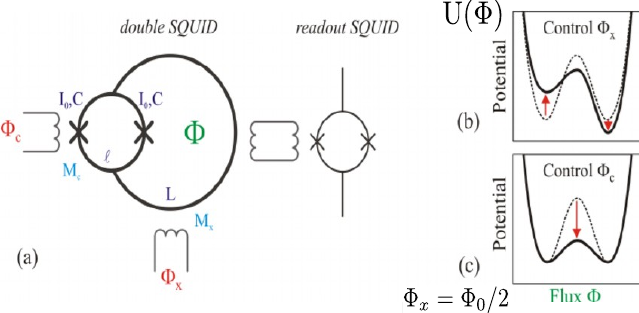
\includegraphics[width=0.8\textwidth]{immagini/flux_qubit_modulation_E_J.png}
\end{figure}
\hspace{-0.6cm}Invece di utilizzare una singola giunzione Josephson, possiamo sostituirla con un piccolo loop contenente due giunzioni Josephson.\\
Questo nuovo elemento si comporta ancora come un elemento Josephson efficace, ma con un'energia Josephson dipendente dal flusso magnetico che attraversa il piccolo loop.\\
In questo modo otteniamo una Josephson energy modulabile.\\
In configurazioni di questo tipo abbiamo quindi due controlli distinti:
\begin{itemize}[leftmargin=0.5cm]
    \item $\Phi_x$, generato dal circuito che produce il flusso principalmente nel loop grande;
    \item $\Phi_c$, prodotto da un secondo circuito accoppiato principalmente al loop piccolo.
\end{itemize}
Possiamo quindi:
\begin{itemize}[leftmargin=0.5cm]
    \item modificare $\Phi_x$;
    \item oppure modulare efficacemente $E_J$ tramite $\Phi_c$.
\end{itemize}
In queste configurazioni i due parametri di controllo permettono quindi di modificare la forma del potenziale oppure, facendoli variare nel tempo, di eseguire operazioni sugli stati del qubit.\\
Ad esempio, variando il bias $\Phi_c$ possiamo modificare l'altezza della barriera del doppio pozzo. In pratica il potenziale può passare:
\begin{itemize}[leftmargin=0.5cm]
    \item da una configurazione a doppio pozzo;
    \item a un potenziale quasi quartico;
    \item fino a una forma quasi armonica;
    \item oppure tornare a un doppio pozzo asimmetrico.
\end{itemize}
Queste modifiche possono essere realizzate sperimentalmente.\\
I due controlli agiscono in modo differente:
\begin{itemize}[leftmargin=0.5cm]
    \item $\Phi_x$ modifica principalmente la simmetria del potenziale;
    \item $\Phi_c$ controlla principalmente l'altezza della barriera.
\end{itemize}
\subsection{Driving e misura}
Abbiamo detto che ci servono due livelli ben definiti e la possibilità di pilotarli. Questo può essere fatto, ad esempio, tramite il flusso magnetico esterno. Inoltre, dobbiamo essere in grado di effettuare la misura del sistema.\\
Gli ingredienti fondamentali sono quindi sempre gli stessi: driving e misura.\\
Per effettuare la misura sfruttiamo il fatto che i due stati del flux qubit corrispondono a differenti correnti che circolano nel circuito.\\
Possiamo quindi accoppiare questo circuito a un secondo loop superconduttivo e misurare il flusso magnetico attraverso tale loop, che dipenderà dallo stato del qubit.\\
Anche in questo caso si tratta quindi di una misura di tipo non demolition. L'accoppiamento con il secondo circuito avviene tramite un'induttanza mutua.\\
Vediamo un possibile circuito realizzato sperimentalmente:
\begin{figure}[H]
    \centering
    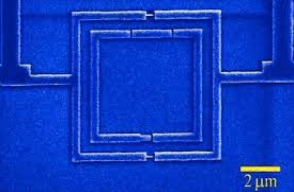
\includegraphics[width=0.5\textwidth]{immagini/flux_qubit_circuit.png}
\end{figure}
\hspace{-0.6cm}La parte interna rappresenta l'anello superconduttivo che realizza il flux qubit, mentre l'anello più grande esterno costituisce il circuito di misura.\\
Quest'ultimo contiene due giunzioni Josephson e viene utilizzato per misurare il flusso magnetico generato dall'anello interno.\\
In pratica, ciò che si misura è il flusso attraverso il loop più grande, che dipende dal flusso magnetico prodotto dalla corrente che circola nell'anello interno.\\
Misurando quindi il flusso — oppure equivalentemente la corrente che circola nel loop esterno — possiamo determinare lo stato dell'anello interno, che, se correttamente polarizzato, può trovarsi soltanto in due stati distinti.
\section{Tempo di vita dei qubit}
Consideriamo ora l'evoluzione di questi qubit nel corso degli anni.
\begin{figure}[H]
    \centering
    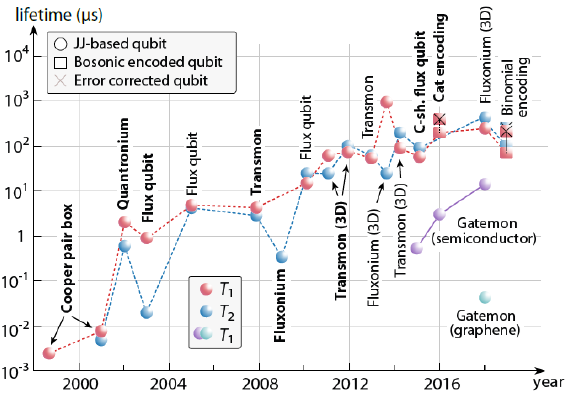
\includegraphics[width=0.7\textwidth]{immagini/qubit_lifetime.png}
\end{figure}
\hspace{-0.6cm}Qui vediamo il cosiddetto tempo di vita del qubit (\emph{qubit lifetime}) in funzione dell'anno in cui il dispositivo è stato realizzato.\\
Il tempo di vita del qubit è una misura di quanto rapidamente decadano nel tempo le oscillazioni coerenti del sistema. Abbiamo infatti visto, nel caso del charge qubit e del flux qubit, che le oscillazioni che descrivono il passaggio coerente del qubit tra i due stati non persistono indefinitamente: invece di oscillare periodicamente per sempre, esse decadono nel tempo secondo una certa legge di decadimento, spesso di tipo esponenziale, caratterizzata da una scala temporale chiamata $T_1$.\\
Nel grafico è riportato proprio questo tempo di vita $T_1$ per differenti tipi di qubit.\\
Vediamo innanzitutto il Cooper pair box, cioè il primo dispositivo che abbiamo discusso, con tempi di coerenza dell'ordine dei nanosecondi, addirittura inferiori a $10\,\mathrm{ns}$.\\
Successivamente, passando al quantronium e poi al transmon, osserviamo un aumento del tempo di rilassamento di circa tre o quattro ordini di grandezza. Analogamente, anche altre tipologie di qubit mostrano un miglioramento progressivo nel tempo.\\
Questo incremento del tempo di coerenza è il risultato di differenti sforzi sperimentali, riconducibili principalmente a due strategie:
\begin{itemize}[leftmargin=0.5cm]
    \item ridurre le sorgenti di rumore;
    \item ottimizzare il dispositivo e il suo controllo.
\end{itemize}
Ridurre il rumore significa innanzitutto utilizzare materiali migliori, dove ``migliori'' significa soprattutto materiali con un numero minore di difetti.\\
Inoltre, si possono utilizzare configurazioni circuitali migliori, cioè progettare il dispositivo in modo da renderlo meno sensibile alle sorgenti di rumore. Un esempio importante di questa strategia è proprio il transmon.\\
Questa è quindi una prima linea di intervento.\\
La seconda consiste invece nell'ottimizzazione dinamica del dispositivo, ad esempio tramite controlli dipendenti dal tempo come tensioni o flussi magnetici. In pratica, si utilizzano segnali di controllo opportunamente progettati per ridurre l'effetto delle sorgenti di rumore.\\
Questa ottimizzazione può essere realizzata con approcci differenti, anche numerici, utilizzando tecniche di intelligenza artificiale o machine learning.\\
Tutto questo serve a sottolineare che questi circuiti, chiamati spesso atomi artificiali superconduttivi, sono fortemente influenzati da sorgenti di rumore che derivano dai materiali microscopici utilizzati per realizzare il circuito stesso.\\
Pensiamo, ad esempio, al Cooper pair box. La giunzione tunnel e gli elettrodi superconduttivi sono tipicamente depositati sopra un substrato dielettrico. In questi materiali — sia nello strato isolante sia nel substrato — possono essere presenti impurità e difetti strutturali.\\
Abbiamo infatti detto che una giunzione Josephson, nella sua implementazione più semplice, è ottenuta depositando due strati superconduttivi separati da un ossido sottile. Questo ossido costituisce la barriera attraverso la quale avviene l'effetto Josephson.\\
Sia nell'ossido sia nel substrato possono quindi essere naturalmente presenti difetti. Alcuni di questi difetti possono essere carichi elettricamente.\\
Possiamo pensare, ad esempio, a una giunzione Josephson in alluminio:
\begin{itemize}[leftmargin=0.5cm]
    \item abbiamo gli elettrodi di alluminio;
    \item tra essi è presente uno strato di ossido di alluminio;
    \item idealmente l'ossido dovrebbe essere un cristallo regolare;
    \item tuttavia possono comparire difetti configurazionali.
\end{itemize}
Questi difetti possono essere schematizzati come minimi addizionali del potenziale all'interno dello strato isolante. Una carica può allora localizzarsi in uno oppure nell'altro di questi minimi.\\
A seconda della posizione occupata dalla carica, cambia la polarizzazione dell'isola superconduttiva.\\
Questo accade perché il dispositivo è estremamente piccolo, tipicamente dell'ordine di pochi nanometri, e quindi anche una singola carica può influenzare significativamente il potenziale elettrostatico dell'isola.\\
Queste impurità, chiamate \emph{background charges}, possono fluttuare nel tempo:
\begin{itemize}[leftmargin=0.5cm]
    \item la carica può trovarsi in una configurazione;
    \item poi passare all'altra;
    \item e così via.
\end{itemize}
In questo modo esse inducono una polarizzazione fluttuante dell'isola superconduttiva.\\
In pratica non è presente un singolo difetto ma un gran numero di difetti, che producono un rumore nella polarizzazione dell'isola con spettro caratteristico di tipo $\frac{1}{f}$, cioè un rumore che cresce fortemente alle basse frequenze.\\
Questa è una delle principali sorgenti di rumore negli atomi artificiali superconduttivi e, in particolare nel charge qubit, è responsabile del rapido decadimento delle oscillazioni coerenti.\\
Nella prima generazione di qubit superconduttivi questo tipo di rumore era estremamente dannoso ed era la principale limitazione sperimentale.\\
Il miglioramento dei charge qubit è quindi dovuto sia:
\begin{itemize}[leftmargin=0.5cm]
    \item all'ottimizzazione del design del dispositivo;
    \item sia all'utilizzo di materiali migliori.
\end{itemize}
Queste sono proprio le due strategie che abbiamo discusso prima:
\begin{itemize}[leftmargin=0.5cm]
    \item riduzione del rumore tramite materiali migliori;
    \item ottimizzazione del dispositivo tramite progettazione circuitale e tecniche di controllo.
\end{itemize}
Questo tipo di rumore a spettro $1/f$ è tipico delle implementazioni basate sulla carica, ma è presente anche nei flux qubit e nei phase qubit.\\
Consideriamo ora due difetti carichi. Essi costituiscono essenzialmente un dipolo elettrico, che può oscillare nel tempo.\\
Abbiamo già detto che, nei dispositivi con isola superconduttiva, l'oscillazione bistabile di una singola carica all'interno della giunzione può produrre una polarizzazione fluttuante dell'isola. Questa è precisamente l'origine del rumore di carica associato alle fluttuazioni della polarizzazione.\\
Processi di questo tipo possono influenzare anche la corrente critica della giunzione.\\
Ricordiamo infatti che la corrente critica è la massima supercorrente che la giunzione può sostenere e dipende dalle proprietà microscopiche della giunzione stessa.\\
Se all'interno del materiale che costituisce la giunzione sono presenti dipoli fluttuanti, possiamo pensare che tali fluttuazioni modifichino localmente la trasparenza della giunzione, e quindi il valore massimo di supercorrente sostenibile.\\
Le fluttuazioni dei dipoli inducono quindi anche fluttuazioni della corrente critica.\\
Tali fluttuazioni sono state osservate sperimentalmente e mostrano anch'esse uno spettro con forti componenti a bassa frequenza.\\
Tutto questo serve a dire che tutte le implementazioni menzionate — charge, flux e phase qubit — soffrono di rumore con spettro $1/f$, generato da differenti meccanismi microscopici:
\begin{itemize}[leftmargin=0.5cm]
    \item alcuni relativamente ben compresi;
    \item altri ancora oggetto di studio teorico e sperimentale.
\end{itemize}
Processi di questo tipo sono presenti anche in giunzioni Josephson basate su grafene:
\begin{figure}[H]
    \centering
    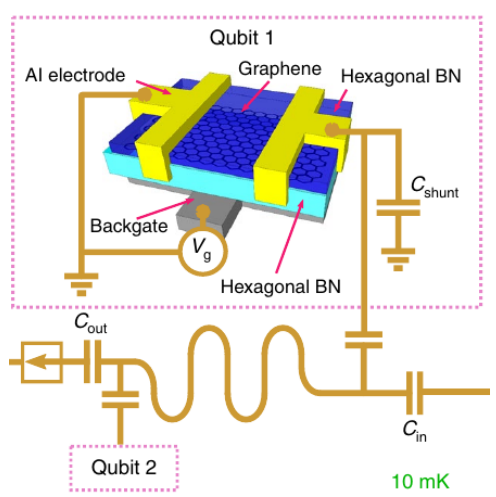
\includegraphics[width=0.5\textwidth]{immagini/graphene_junction.png}
\end{figure}
\hspace{-0.6cm}In questo caso abbiamo uno strato di grafene posto tra due strati di nitruro di boro esagonale, che lo isolano molto bene, mentre i contatti superconduttivi sono realizzati lateralmente quasi in geometria unidimensionale.\\
Quando questa giunzione viene inserita in un circuito, può essere controllata tramite una tensione di gate e il dispositivo viene chiamato \emph{gatemon}, poiché è molto simile al transmon, con la differenza principale che la giunzione Josephson tradizionale è sostituita da una giunzione Josephson a grafene.\\
Anche in questo caso il sistema è sensibile a diverse sorgenti di fluttuazione, ad esempio fluttuazioni della densità di portatori nel grafene.\\
Infatti il grafene possiede una certa densità elettronica che può fluttuare nel tempo e, quando questo elemento viene utilizzato all'interno della giunzione Josephson, tali fluttuazioni introducono rumore nel circuito.\\
Questo tipo di rumore è simile a quello presente nei dispositivi CMOS a semiconduttore.\\
In generale, quando sono presenti ossidi, esistono impurità e trappole di carica. Nei dispositivi CMOS, ad esempio, la corrente dovrebbe fluire dal source al drain, ma se esistono trappole di carica nell'ossido alcune cariche possono venire intrappolate invece di attraversare il canale.\\
Questo processo produce rumore nella corrente.\\
Se esiste un gran numero di trappole distribuite casualmente nello strato isolante, la combinazione dei processi di intrappolamento produce un rumore con spettro $\frac{1}{f}$.\\
Si tratta quindi di un fenomeno estremamente generale nei dispositivi a stato solido:
\begin{itemize}[leftmargin=0.5cm]
    \item transistor a semiconduttore;
    \item circuiti superconduttivi;
    \item dispositivi per tecnologie quantistiche;
    \item altri sistemi artificiali nanostrutturati.
\end{itemize}